\documentclass[11pt]{article}

\usepackage{xcolor}
\usepackage{mathtools}
\usepackage[legalpaper, margin=1in]{geometry}
\usepackage{amsmath}
\usepackage{amssymb}
\usepackage{paralist}
\usepackage{rsfso}
\usepackage{amsthm}
\usepackage[inline]{enumitem}   

\newtheoremstyle{break}
  {\topsep}{\topsep}%
  {\itshape}{}%
  {\bfseries}{}%
  {\newline}{}%
\theoremstyle{break}
\theoremstyle{break}
\newtheorem{axiom}{Axiom}
\newtheorem{thm}{Theorem}[section]
\newtheorem{lem}{Lemma}[thm]
\newtheorem{prop}[lem]{Proposition}
\newtheorem{corL}{Corollary}[lem]
\newtheorem{corT}[lem]{Corollary}
\newtheorem{defn}{Definition}[corL]

\newcommand{\R}{\mathbb{R}}
\newcommand{\N}{\mathbb{N}}
\newcommand{\Z}{\mathbb{Z}}
\newcommand{\Q}{\mathbb{Q}}
\newcommand{\A}{\mathcal{A}}
\newcommand{\J}{\mathcal{J}}
\newcommand{\T}{\mathcal{T}}
\newcommand{\Td}{\mathcal{T}_d}
\newcommand{\C}{\mathcal{C}}
\newcommand{\M}{\mathcal{M}}
\newcommand{\Complex}{\mathbb{C}}
\newcommand{\Power}{\mathcal{P}}
\newcommand{\ee}{\cdot 10}
\newcommand{\Intab}{[\,a,b\,]}
\newcommand{\vmat}[1]{\begin{vmatrix} #1 \end{vmatrix}}
\newcommand{\bmat}[1]{\begin{bmatrix} #1 \end{bmatrix}}
\newcommand{\pmat}[1]{\begin{pmatrix} #1 \end{pmatrix}}

\makeatletter
\def\@seccntformat#1{%
  \expandafter\ifx\csname c@#1\endcsname\c@section\else
  \csname the#1\endcsname\quad
  \fi}
\makeatother

\makeatletter
\newcommand*{\rom}[1]{\expandafter\@slowromancap\romannumeral #1@}
\makeatother

\makeatletter
% This command ignores the optional argument for itemize and enumerate lists
\newcommand{\inlineitem}[1][]{%
\ifnum\enit@type=\tw@
    {\descriptionlabel{#1}}
  \hspace{\labelsep}%
\else
  \ifnum\enit@type=\z@
       \refstepcounter{\@listctr}\fi
    \quad\@itemlabel\hspace{\labelsep}%
\fi}
\makeatother
\parindent=0pt


\begin{document}

	\begin{titlepage}
		\begin{center}
			\topskip0pt
			\vspace*{\fill}
			\Huge \color{red}
				\textbf{Class Notes}\\
			\vspace{0.5cm}			
			\Large \color{black}
				Physics 360 - Honors Physics III\\	
				University of Michigan\\
			\vspace{3cm}
			
			
\includegraphics[scale=0.8]{hmm.pdf}
			
			\vspace{5cm}
			\LARGE
				\textbf{Jinyan Miao}\\
				Fall 2021\\
			\vspace{5cm}

		\vspace*{\fill}
		\end{center}			
	\end{titlepage}

\newpage
\Large\textbf{}\\
\normalsize 

\textbf{A Brief history of Physics:}\\
1600s \hfill	Newtonian Mechanics by Isaac Newton\\
1800-1875 \hfill Electromagnetism by J.C. Maxwell\\
1850-1900\hfill Thermodynamics and Statistical Mechanics\\
1905\hfill Special Relativity by Einstein\\
1915\hfill General Relativity by Einstein\\
1900-today\hfill Quantum Mechanics\\
1920-today\hfill Quantum Field Theory\\
1980-today\hfill String Theory\\

\newpage
\section{\color{red}Special Relativity}
\hfill\break
\textbf{Coordinate Transformation}\\
In two dimensional frames, say we have one frame $F(x,y)$ and another frame $\widetilde{F}(\widetilde{x},\widetilde{y})$, then the change in coordinate, or the shift, or the translation, can usually expressed by $\widetilde{x}=x+x_0$, $\widetilde{y} = y+y_0$ for some constant $x_0$ and $y_0$.\\

The physical laws are invariant under coordinate transformation, but the initial conditions are in general not invariant, such as the height of a ball in different frames.\\

\hfill\break
\textbf{Galilean Transformation}\\
Now suppose, in frame $S$, a train moves at speed $u$ in the $x$-direction, the train starts at $x=0$ at $t=0$, then the position of the train is $x=ut$ in frame $S$. In another frame $S'$, the moving frame of the train, at all times $t'$, the position of the train is $x'=0$. Here we can write the Galilean Transformation as the following, from frame $S(x,y,z,t)$ to $S'(x',y',z',t')$:
\begin{align*}
x'=x-ut \qquad \qquad y'=y \qquad\qquad z'=z \qquad \qquad t'=t
\end{align*}
Now suppose a person comoving with the train, which is moving as a speed $u$ as seen from the frame $S$ in the $x$-direction, throws a ball at a speed $v'$ as seen in the frame $S'$ in the $x'$-direction. From Galilean Transformation, we can write the speed of the ball as the following:\\$$\text{In S':}\qquad v' = \frac{dx'}{dt'} = \frac{dx'}{dt}\qquad\qquad\qquad\qquad\qquad\qquad\qquad \text{In S:} \qquad v = \frac{dx}{dt}$$
$$v = \frac{dx}{dt} = \frac{d}{dt}(x'+ut) = v'+u$$
Hence in Galilean Transformation, we have $v = v'+u$\\
For acceleration in Galilean Transformation, we can write the followings:
$$a = \frac{d^2x}{dt^2} = \frac{d^2}{dt^2}(x'+ut) = \frac{d^2x'}{dt^2} = \frac{d^2x'}{dt'^2} = a'$$
where $a$ is the acceleration in $S$ and $a'$ is the acceleration in $S'$. Hence we conclude that $a=a'$ in Galilean Transformation.\\

For Newton's Second Law in Galilean Transformation, we can write the following:
$$F = ma = ma'$$
Hence force is invariant in all frames under Galilean Transformation.\\

EX. Hook's Law: $F=k(x_1-x_2)=k(x_1'-x_2')$\\
EX. Newton's Gravity: $F = G\frac{mM}{|r_1-r_2|^2}= G\frac{mM}{|r_1'-r_2'|^2}$\\

Here we note that Newton's Laws are invariant under Galilean Transformation.\\
While in general, the wave equation for electromagnetic waves is not invariant under Galilean Transformation.\\
\newpage
\textbf{Lorentz Transformation}\\
Consider we have a train moving at a speed $u$ as seen from a frame $S(x,y,z,t)$ in the $x$-direction. The frame of the train is $S'(x',y',z',t')$. A person on the train shines a flashlight in the $x'$-direction as seen in the frame $S'$. Here under Galilean Transformation, the speed of the light in frame $S'$ is $c$, then the speed of light in frame $S$ will be $c+u\neq c$. However, experimentally, the speed of light is the same in all inertial frames. Hence Galilean transformations are incompatible with the speed of light being the same in all inertial frames.\\

Special relativity builds on Einstein's two Postulates:
\begin{enumerate}[topsep=3pt,itemsep=-1ex,partopsep=1ex,parsep=1ex]
\item \textbf{Principle of Relativity}: The laws of physics are the same in every inertial frames.
\item \textbf{Speed of light is constant}: The speed of light in vacuum is the same in all inertial frames and is independent of the motion of the light source.
\end{enumerate}

In special relativity, we use the Lorentz Transformation instead of the Galilean Transformation.\\

Suppose we have inertial frame $S(x,y,z,t)$ and inertial frame $S'(x',y',z',t')$ which is moving at a speed $u$ in the $x$-direction as seen from the frame $S$. The Lorentz Transformation says the following:
$$x' = \frac{x-ut}{\sqrt{1-\frac{u^2}{c^2}}}\qquad\qquad y=y'\qquad\qquad z'=z\qquad\qquad t'=\frac{t-\frac{u}{c^2}x}{\sqrt{1-\frac{u^2}{c^2}}}$$

Here we can define $\beta$ and a Lorentz Factor $\gamma$ to clear things up:
$$\beta = \frac{u}{c}\qquad\qquad\qquad \gamma = \frac{1}{\sqrt{1-\beta^2}}$$
Then we can rewrite the Lorentz Transformation as the following:
$$x' = \gamma(x-ut)\qquad\qquad y'=y\qquad\qquad z'=z\qquad\qquad t'=\gamma(t-\frac{u}{c^2}x)$$

\newpage
\textbf{Lorentz Velocity Transformation}\\
Here we will derive the Lorentz velocity Transformation. Suppose a ball is moving in the $S'$ frame with a speed $v_x'=\frac{dx'}{dt'}$, we want to find the speed of the ball in $S$ frame, denoted as $v_x = \frac{dx}{dt}$.

$$\frac{dx'}{dt} = \frac{d}{dt}(\gamma(x-ut)) = \gamma(\frac{dx}{dt}-u) = \gamma(v_x-u)$$
$$\frac{dt'}{dt} = \frac{d}{dt}(\gamma(t-\frac{u}{c^2}x)) = \gamma(1-\frac{u}{c^2}\frac{dx}{dt}) = \gamma(1-\frac{uv_x}{c^2})$$
$$v_x' = \frac{dx'}{dt'} = \frac{\left(\frac{dx'}{dt}\right)}{\left(\frac{dt'}{dt}\right)} = \frac{\gamma(v_x-u)}{\gamma(1-\frac{uv_x}{c^2})} = \frac{v_x-u}{1-\frac{uv_x}{c^2}}$$
Here we note that, we assume $v_x'$, $v_x$, $u$ are all in the $x$-direction.

Here we will derive the velocity transformation for the $y$ and $z$ components of the velocity. Suppose the the ball is also moving in the $S$ frame with a speed $v_y=\frac{dy}{dt}$ in $y$ direction, and $v_z = \frac{dz}{dt}$ in $z$ direction, we want to find the speed of the object in $S'$ frame, denoted as $v_y' = \frac{dy'}{dt'}$, and $v_z' = \frac{dz'}{dt'}$. The two frames, $S$ and $S'$, are in relative motion in the $x$-direction at the speed $u$.

$$\frac{dy'}{dt} = \frac{d}{dt}(y') =\frac{d}{dt}y = \frac{dy}{dt} = v_y$$
$$\frac{dt'}{dt} = \frac{d}{dt}(\gamma(t-\frac{u}{c^2}x)) = \gamma(1-\frac{u}{c^2}\frac{dx}{dt}) = \gamma(1-\frac{uv_x}{c^2})$$
$$v_y' = \frac{dy'}{dt'} = \frac{\left(\frac{dy'}{dt}\right)}{\left(\frac{dt'}{dt}\right)} = \frac{v_y}{\gamma(1-\frac{uv_x}{c^2})} $$

$$\frac{dz'}{dt} = \frac{d}{dt}(z') =\frac{d}{dt}z = \frac{dz}{dt} = v_z$$
$$\frac{dt'}{dt} = \frac{d}{dt}(\gamma(t-\frac{u}{c^2}x)) = \gamma(1-\frac{u}{c^2}\frac{dx}{dt}) = \gamma(1-\frac{uv_x}{c^2})$$
$$v_z' = \frac{dz'}{dt'} = \frac{\left(\frac{dz'}{dt}\right)}{\left(\frac{dt'}{dt}\right)} = \frac{v_z}{\gamma(1-\frac{uv_x}{c^2})} $$

Notice here, in Galilean Transformation, we have $v_x' = v_x-u$, while in Lorentz Transformation, we have $v_x' = \frac{v_x-u}{1-\frac{uv_x}{c^2}}$. In the case where $u<<c$, we have $\frac{u}{c}<<1,\ |\frac{v_x}{c}|\leq 1 \Rightarrow 1-\frac{uv_x}{c^2}\approx 1$, that is, when $u<<c$, Lorentz Transformation yields around the same results as Galilean Transformation.\\

In Lorentz Transformation, $v_x'\leq c$ holds true all the time.\\ 

On another note, if we have $v_x = c$, from Lorentz Transformation, we have $v_x' = \frac{c-u}{1-\frac{u}{c}} = c$, which indicates that if something moves at the speed of light in one frame, it has to move at the speed of light in all frames. On the other hand, if something moves at a speed less than the speed of light in one frame, then it must move at a speed less than the speed of light in all frames.
\newpage

\textbf{Time Dilation}\\
\begin{defn}
An event is something that happens at a point in space $(x,y,z)$ at a given time $t$. In a different inertial frame, the event happens at $(x',y',z')$ at a time $t'$.
\end{defn}

Consider that in frame $S'(x',y',z',t')$, there are two events happen at the same location at $(x',y',z')$, but at different times $t'_1$ and $t'_2$. So here we have event 1 denoted as $(x',y',z',t'_1)$ and event 2 denoted as $(x',y',z',t'_2)$. A clock at rest in $S'$ that goes "tick" at $t'_1$ and "tick" again at $t'_1$. An observer at rest in $S'$ will see the time between the "ticks" as $T_0 = \Delta t' = t'_1-t'_2$. Suppose in another frame $S$, moving as a speed $u$ relative to $S'$ as seen by someone at rest in $S$ in the $x$-direction. Here we have the following:
$$t_1 = \gamma(t'_1+\frac{u}{c^2} x') \qquad \qquad t_2 = \gamma(t'_2+\frac{u}{c^2} x')$$
where we have $x' = x'_1=x'_2$, hence we can conclude the following:
$$T = \Delta t = t_2 - t_1 = \gamma (t'_2 - t'_1) = \gamma \Delta t' = \gamma T_0$$
Here we note that $\gamma \geq 1$, hence we have $T \geq T_0$, which indicates that observer in rest in $S$ sees the moving clock in $S'$ ticks slower. On another note, $T_0$, which is the time seen in the rest frame, relative to the events, is called the Proper Time.\\

EX. A plane travels from San Francisco to New York City, a distance around $L=4800km$, at the speed around $u = 245m/s$. Let the Earth be the frame $S(x,y,z,t)$. In $S$, it takes $T = \Delta t = \frac{L}{u} = 19.6\cdot 10^3 s$ to travel. Let the moving plane be frame $S'(x',y',z',t')$. In $S'$, we have $T_0 = \Delta t' = \frac{1}{\gamma} T$, but here we have $\beta << 1$ and hence $\gamma \approx 1$, hence we will have $\Delta t' = \frac{1}{\gamma}T \approx \Delta t = T_0$. We see that the effect of special relativity for such an example is very small. But we can still write the following: $$\frac{1}{\gamma} = \sqrt{1-\beta^2}\approx 1-\frac{1}{2}\beta^2+ O(\beta^4) \qquad \Rightarrow \qquad T_0 = \frac{1}{\gamma}T = T-\frac{1}{2}\beta^2 T$$
$$T-T_0 = \frac{1}{2}\beta^2 T \approx \frac{1}{2}(10^{-6})^2(196\cdot 10^3 s) \approx 6\cdot 10^{-9}s \approx 6\ nanoseconds$$
Sending a plane all the way around the Earth will take around instead, we will have $T = \frac{40\cdot 10^6m}{245m/s} \approx 1.63\cdot 10^5 s$, and we have $T-T_0 \approx \frac{ 1}{2}\beta^2 T \approx 54\ nanoseconds$ in this case. This effect is indeed measurable, observed in 1971.\\

Here we note that, in general, we use $T_0$ to denote the proper time, which is the time measured in the rest frame, that is, the time measured in the frame in which the event starts and ends at the same place. By the time dilation formula, we have $T= \gamma T_0$, where $\gamma \geq 1$ always, so an observer will see time on a moving clock go slower, that is, we have $T \geq T_0$ always. \\

Time dilation can be verified by taking atomic clocks on board planes moving around the Earth. We might also use particle physics, the muon decays to detect the time dilation effect. Also, time dilation is important for the GPS system to work.\\


\textbf{\textit{A moving clock ticks slower.}}

\newpage
\textbf{Twin Paradox}\\
Consider two twins, $E$ and $S$, $E$ stays on Earth, and $S$ goes on a rocket travels to a star far away, then comes back. The rocket goes away from the Earth at a speed $u=0.99c$. $S$ says the time on his clock goes $5$ years in total, from the Earth to the star and back to the Earth. From the previous result, we know that $E$'s clock has goes $T = \gamma T_0 = \gamma \cdot 5\ years \approx 35\ years$.\\

However, we can also consider the following statement:\\

\textit{The Earth is moving away from the rocket, and $S$ says it takes 5 years to travel. In this case, $E$ would say his clock only goes $T_0 = \frac{T}{\gamma}=\frac{5\ years}{\gamma} \approx 0.71\ years$}\\

This statement is not correct, this is because $S$ has to change the direction of his rocket to come back to the Earth, and hence his frame experiences acceleration during his trip, such case can be explained using the theory of General Relativity. As a result, we will have $T$ being 35 years. And in fact there is no paradox. 



\newpage
\textbf{Length Contraction}\\
Here we will derive length contraction for special relativity. Suppose we have two frames in relative motion, $S'(x',y',z',t')$ is moving away from $S(x,y,z,t)$ in the $x$-direction at a speed $u$. A measure stick at rest in $S'$, which endpoints are at $x_1'$ and $x_2'$, then observer at rest in $S'$ sees the length of the measure stick as the following: 
$$L_0 = x_2'-x_1' = \gamma((x_2-x_1)-u(t_2-t_1))$$
Here $L_0$ is the proper length of the stick. In $S$, we assume that an observer at rest in $S$ will see the stick at $t= t_1 = t_2$, so he will measure the length of the stick as the following:
$$L = x_2-x_1\qquad \Rightarrow\qquad L_0 = \gamma L\qquad \Rightarrow\qquad L = \frac{L_0}{\gamma}$$

Recall that $\gamma \geq 1$, so we have $L_0 \geq  L$. Hence an observer at rest in $S$ sees a moving stick length contracted. Also note that, length contraction happens in the direction of the motion, and it does not happen in perpendicular direction, because nothing happens in the $y$ or $z$ direction under Lorentz Transformation when the two frames are in relative motion in $x$ direction only.\\

\textbf{\textit{A moving object looks shorter.}}
\hfill\break
\hfill\break
Example. \\
Two spaceships, observed by a person $C$ at rest in frame $S_C$, one spaceship $A$ is moving at a speed $v$ to the right as seen by $C$ in $S_C$, the other spaceship $B$ is moving at a speed $2v$ to the right as seen by $C$ in $S_C$. As seen by $C$, spaceship $B$'s clock ticks slower. Now suppose the two spaceships have the same size $L_0$, measured in the their rest frames, then as seen by $C$, spaceship $B$ looks shorter in the direction of motion. Note here, $C$ sees $L_A = \sqrt{1-\frac{v^2}{c^2}}L_0$ for spaceship $A$, and sees $L_B = \sqrt{1-\frac{4v^2}{c^2}}L_0$ for spaceship $B$. On another note, as seen by $B$, $C$'s clock ticks the slowest. As seen by $A$, $B$ and $C$'s clock ticks at the same pace.\\


\newpage
\textbf{Space-time Diagram}\\
Suppose we have an object in motion at a constant speed $v$. Here the position of the object can be expressed as the following:
\begin{align}
x = vt+x_0
\end{align}
where $x_0$ is the location of the object at $t=0$. Here we can manipulate equation (1) to get:
$$t = \frac{1}{v}x-\frac{1}{v}x_0\qquad \Rightarrow \qquad ct = \frac{c}{v}x-\frac{c}{v}x_0$$
Now we can let $ct$ to be the vertical axis, and let $x$ to be the horizontal axis, such diagram is called the space-time diagram. Then the motion of the object can be expressed as a function of $x$, which has a slope of $\frac{c}{v}$ and vertical axis interception $-\frac{c}{v}x_0$. A light traveling in the $x$ direction in a space-time diagram has a slope of $\pm 1$\\

If we have something moving at a speed $v$ less than $c$, then $ct = \frac{c}{v}x$ can describe the motion of that object and the equation has a slope $\frac{c}{v}$ greater than $1$.\\

Suppose an event goes from the origin $A$ of the space-time diagram, then the event can travel to a point $B$ in the space time diagram shows by the following:\\
\begin{center}
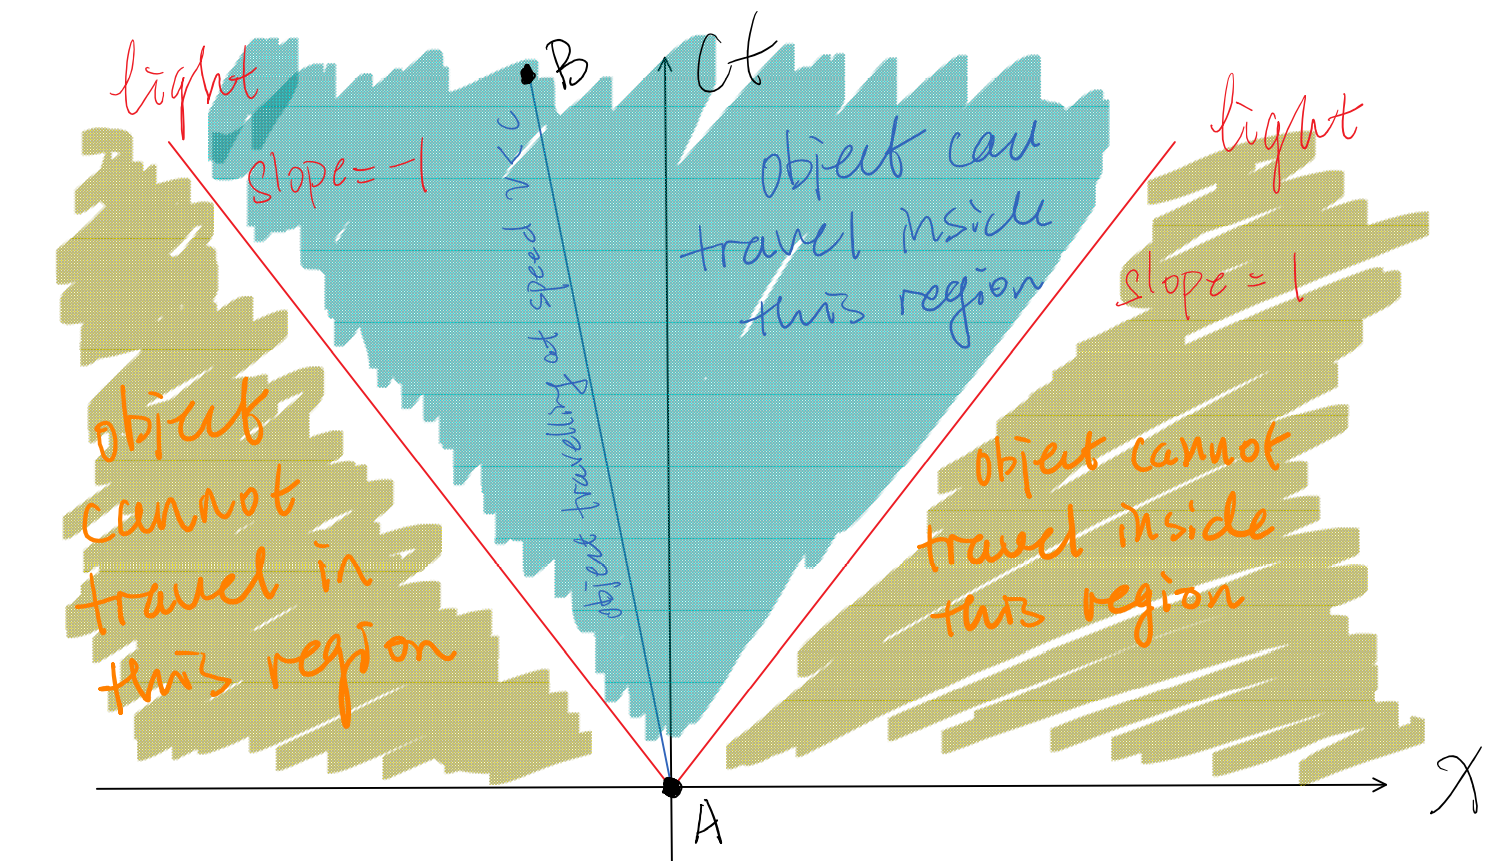
\includegraphics[scale=0.3]{Screenshot (634).png}
\end{center}
That being said, the causal connection of $B=(x_B,ct_B)$ to $A=(0,0)$ is $x_B^2 < c^2t_B^2$. If such $A$ and $B$ are transformed to another frame under Lorentz Transformation, to $A'=(x_A',ct_A')$ and $B'=(x_B',ct_B')$, $x_B'^2 < c^2t_B'^2$ must also holds.\\







\newpage
\textbf{Simultaneity}\\
\begin{center}
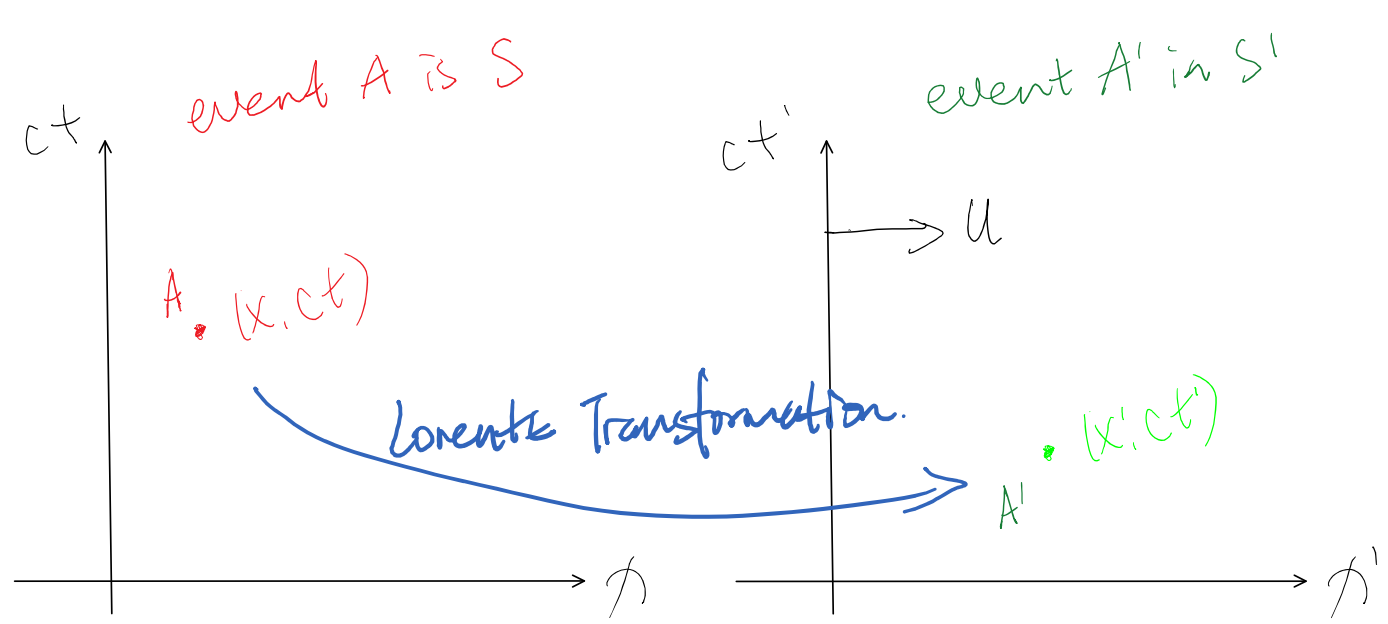
\includegraphics[scale=0.3]{Screenshot (626).png}
\end{center}
Suppose we have two frames, $S(x,y,z,t)$ and $S'(x',y',z',t')$ in relative motion. $S'$ is moving at the speed $u$ in the $x$ direction. Suppose event $A$ happens at $x_A=0$ at time $t=0$ in the frame $S$, and event $B$ happens at $x_B=0$, where $x_0 >0$, at time $t=0$ in the $S$ frame. In $S$, $A$ and $B$ are simultaneously, both happen at time $t=0$. Under Lorentz transformation, $A$ and $B$ are mapped to $A'$ and $B'$ in $S'$. We write the following:
$$A \mapsto A' \begin{cases} x_A' = \gamma (x_A - ut_A) = 0\\ t_A' = \gamma(t_A-\frac{u}{c^2}x_A) = 0\end{cases} \qquad \qquad \qquad B\mapsto B'\begin{cases} x_B'= \gamma(x_B-ut_B) =\gamma x_0 \geq x_0\\ t_B' = \gamma(t_B - \frac{u}{c^2}x_B) = -\gamma\frac{u}{c^2}x_0\leq 0\end{cases}$$
\begin{center}
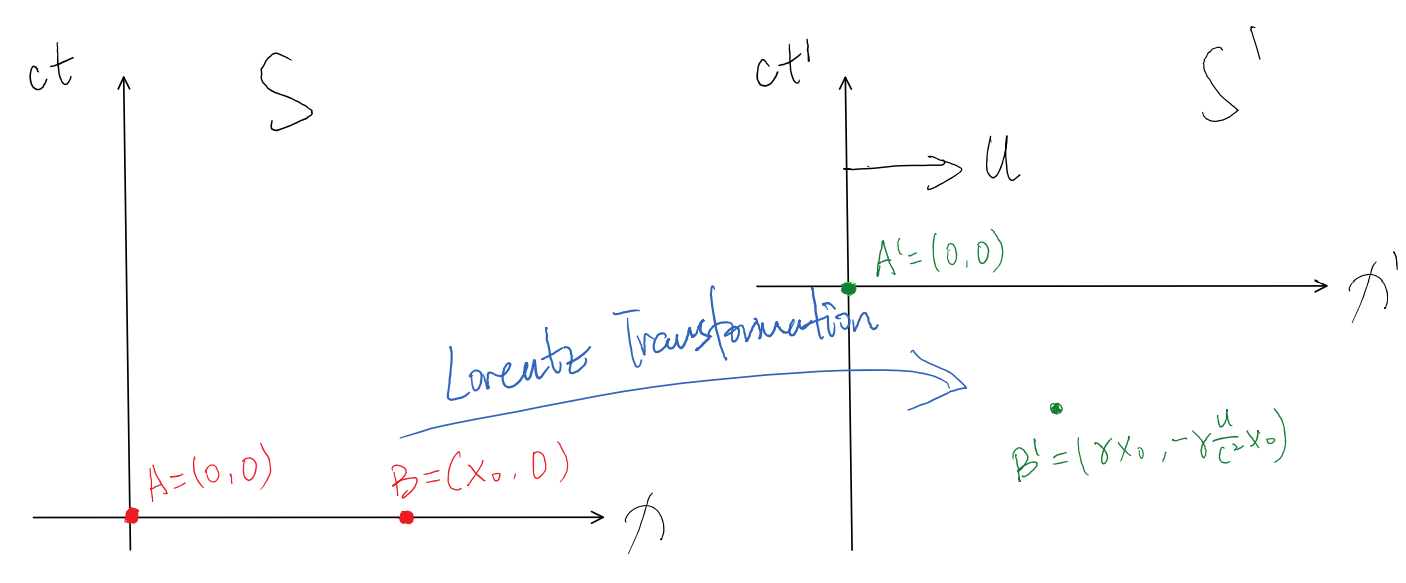
\includegraphics[scale=0.3]{Screenshot (627).png}
\end{center}

Here we see that if $u \neq 0$, then $A'$ and $B'$ are not simultaneous in $S'$ frame. Whether two events are simultaneous depends on the motion of the observers. That is, simultaneity is depending on inertial frame.\\ 






\newpage
Example.\\Suppose we have two rockets, both moving to the right at a speed $u$, measured by a person resting on Earth. One rocket throws a rotten tomato at the speed $v$ to the right, where $v>u$, as measured by the person resting on Earth. Here we can draw a space-time diagram in Earth's rest frame: 
\begin{center}
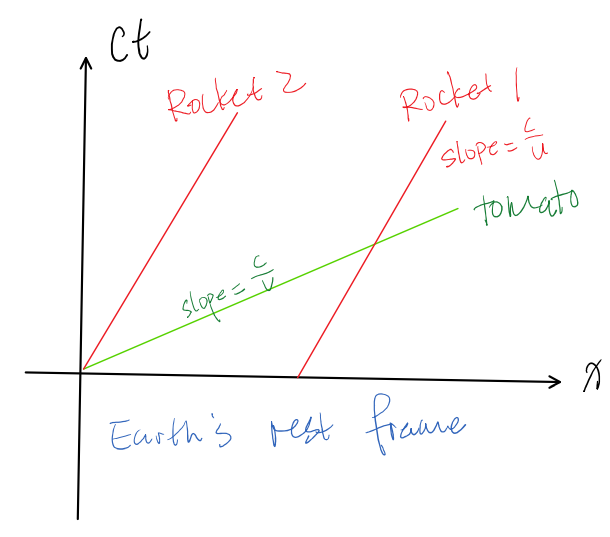
\includegraphics[scale=0.5]{Screenshot (633).png}
\end{center}
We can also draw a space-time diagram in rockets' rest frame.
\begin{center}
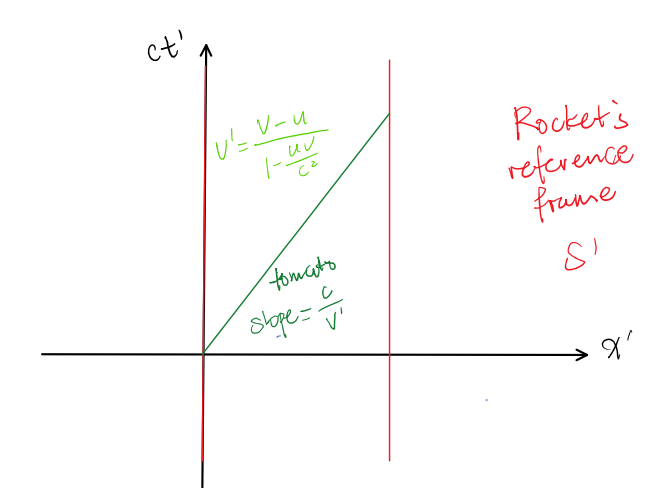
\includegraphics[scale=0.5]{Screenshot (628).png}
\end{center}
And a space-time diagram in tomato's rest frame.
\begin{center}
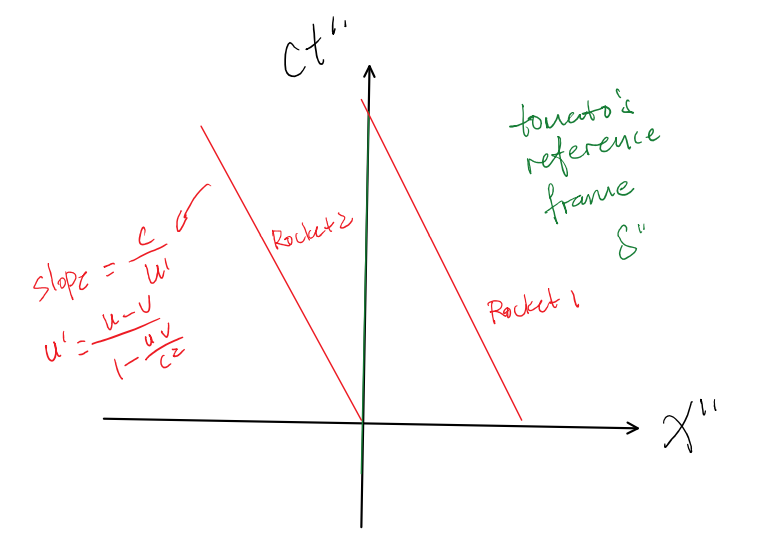
\includegraphics[scale=0.5]{Screenshot (629).png}
\end{center}



\newpage
Example.\\
A person $S$ standing at rest on the ground sees a train pass through at some speed to the right, another person $T$ standing at rest at the middle of the train. When the $x$ position of the two person overlaps, two lightnings strike both
ends of the train.\\

In $S$'s rest frame, we can draw the following space-time diagram. \\
\begin{center}
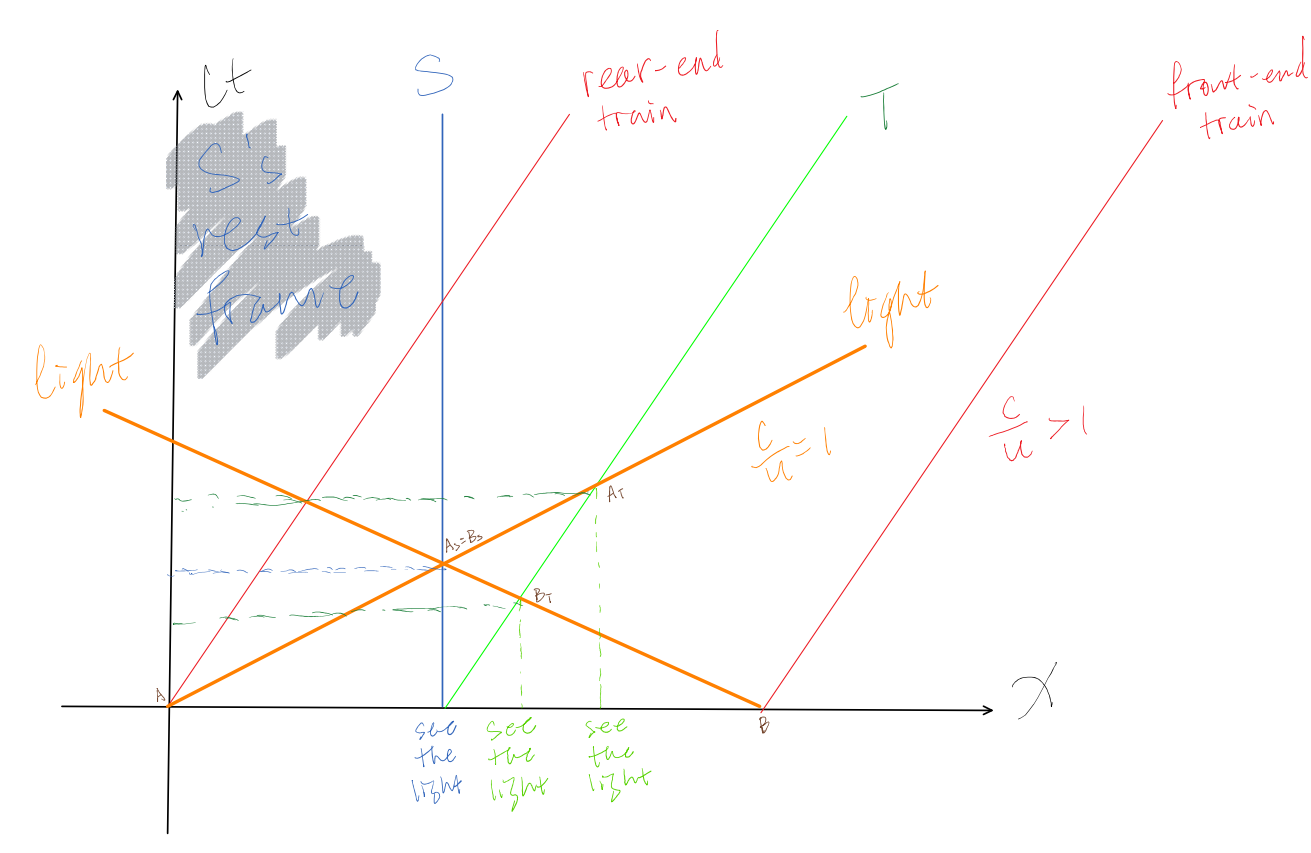
\includegraphics[scale=0.38]{Screenshot (630).png}
\end{center}
To go from $S$'s rest frame to $T$'s rest frame, we apply Lorentz Transformation. In $S$'s frame, he sees the lightning simultaneously, but in $T$'s rest frame, $T$ does not see the two lightning simultaneously. In $T$'s rest frame, we can draw the following space-time diagram.
\begin{center}
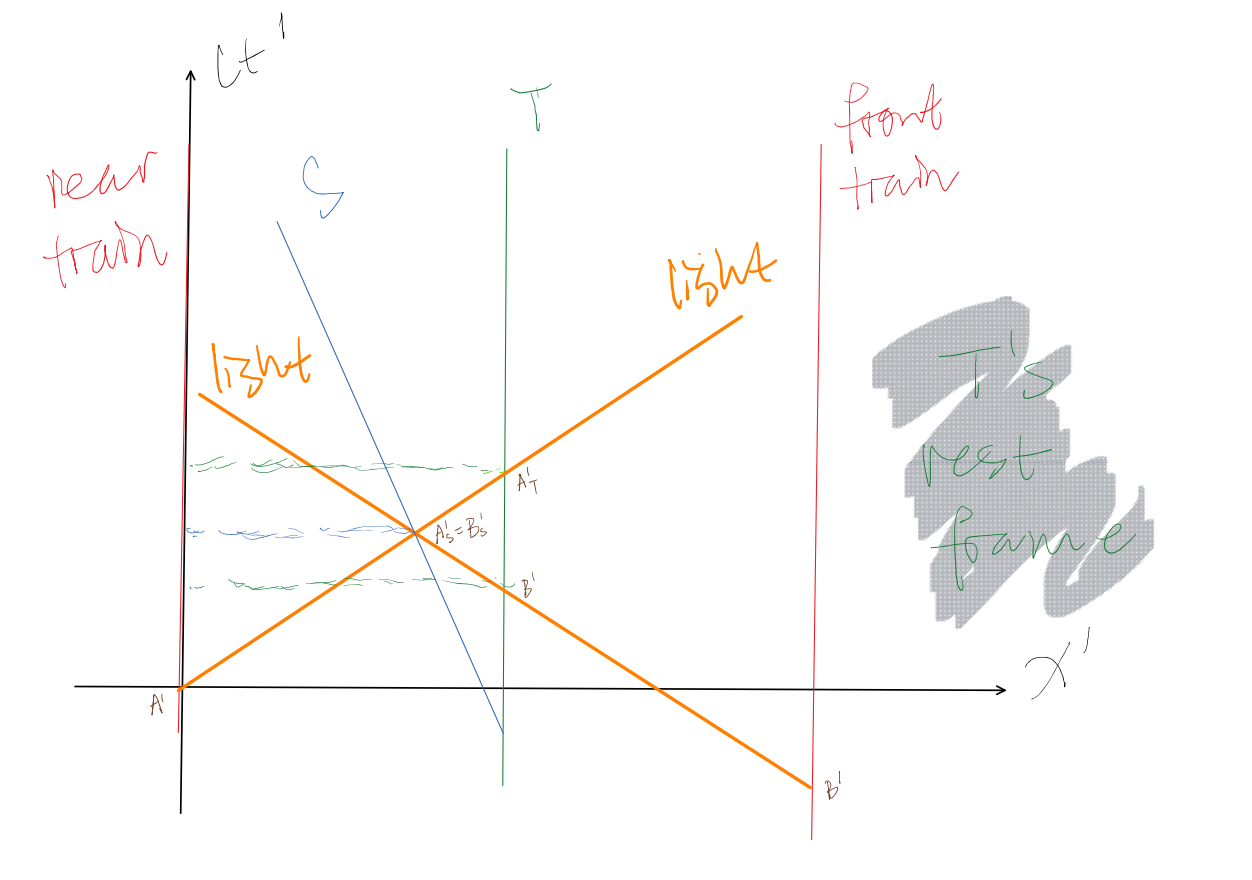
\includegraphics[scale=0.38]{Screenshot (631).png}
\end{center}
Let $A_S,B_S$ represent the events "$S$ sees the light coming from the front of the train" and "$S$ sees the light coming from the rear of the train" in $S$'s rest frame, respectively. Let $A_T,B_T$ represent the events "$T$ sees the light coming from the front of the train" and "$T$ sees the light coming from the rear of the train" in $S$'s rest frame, respectively. Let $A_S',B_S'$ represent the events "$S$ sees the light coming from the front of the train" and "$S$ sees the light coming from the rear of the train" in $T$'s rest frame, respectively. Let $A_T',B_T'$ represent the events "$T$ sees the light coming from the front of the train" and "$T$ sees the light coming from the rear of the train" in $T$'s rest frame, respectively. Let $A,B$, represents the events "the lightning hit the front of the train" and "the lightning hit the back of the train" in $S$'s rest frame, respectively. Let $A',B'$, represents the events "the lightning hit the front of the train" and "the lightning hit the back of the train" in $T$'s rest frame, respectively.\\

Note that, even though $S$ sees $A$, $B$ at the same time, that is, $A$ and $B$ have the same time $t$ in $S$'s rest frame, but $A'$ and $B'$ have different time $t'$ in $T$'s rest frame. In particular, let $A=(0,0)$ and $B=(0,x_0)$, then $B'$ will have a negative time in $T$'s rest frame by our previous result. 

\newpage


\begin{defn}
An inertial frame is an object of no net force acting on it that goes in a straight line.
\end{defn}


In special relativity, one frame $S$ is moving at a speed $u$ relative to the other frame $S'$ in the $x$ direction. Then we can write the following:
$$\vec{a} = \frac{d^2\vec{r}}{dt^2} = \frac{d\vec{v}}{dt} \qquad \qquad \vec{a}' = \frac{d^2\vec{r}'}{dt'^2} = \frac{d\vec{v}'}{dt'}$$
where we have $\vec{v'}=(v_x,v_y,v_z)$, given by the following:
$$\frac{dx'}{dt'} = v_x' = \frac{v_x-u}{1-\frac{uv_x}{c^2}} \qquad \qquad	 \frac{dy'}{dt'} = v_y' = \frac{v_y}{\gamma\left(1-\frac{uv_y}{c^2}\right)} \qquad \qquad \frac{dz'}{dt'}=	v_z' = \frac{v_z}{\gamma\left(1-\frac{uv_z}{c^2}\right)}$$


\begin{defn}
Let $S(x,y,z,t)$ and $S'(x',y',z',t')$ be inertial frames in relative motion at a speed $u$ in the $x$-direction. The spacetime interval $(\Delta s)^2 \coloneqq (c\Delta t)^2 - (\Delta x)^2 - (\Delta y)^2 - (\Delta z)^2$, $(\Delta s')^2 \coloneqq (c\Delta t')^2 - (\Delta x')^2 - (\Delta y')^2 - (\Delta z')^2$
\end{defn}



Notice that, in Lorentz Transformation, the following always holds:
$$(\Delta s')^2 = (\Delta s)^2$$
$$x^2 - c^2 t^2 = x'^2 - c^2 t'^2$$

\newpage
\textbf{Relativistic Momentum}\\
In classical mechanics, the momentum of a moving object with velocity $\vec{v}$ and mass $m$ is given by $\vec{p} = m\vec{v}$, and we can write Newton's Second Law as $\vec{F} = \frac{d\vec{p}}{dt} = d\vec{a}$. In relativity, physical laws must be the same in all inertial frames, including the conservation of momentum.\\

Let $S(x,y,z,t)$ and $S'(x',y',z',t')$ be inertial frames that are in relative motion, $S'$ is moving at a speed $u=0.55c$ in the $x$ direction. In frame $S$, suppose we have a ball $b$ of mass $m$ with speed $v_{1i} = 0.75c$ moving in the positive $x$ direction, and on the right of $b$, we have a ball $B$ of mass $2m$ at rest $v_{2i} = 0$. By the conservation of momentum, without considering the relativistic effect, the final speed of $b$ is $v_{1f} = -0.25c$ in positive $x$ direction, and the final speed of $B$ is $v_{2f} = 0.5c$ in positive $x$ direction. The total momentum of the system is $0.75mc$ before and after the collision. \\

Moving to the frame $S'$, we can write the following:\\
$$v'_{1i} = \frac{v_{1i}-u}{1-\frac{v_{1i}u}{c^2}} = 0.34c \qquad \qquad v'_{2i} = -0.55c$$
where $v_{1i}'$ is the initial speed of the ball $b$ in $S'$, and $v_{2i}'$ is the initial speed of the ball $B$ in $S'$. The initial momentum of the system is then $P_{i}'=-0.76mc$. Similarity, we can find the final velocity of the balls $v'_{1f} = -0.7c$ and $v_{2f} = -0.069c$ by transforming $v_{1f}$ and $v_{2f}$ calculated above. Here the final momentum is given by $P_{f}' = -0.84mc$. We here get $P_{f}' \neq P_{i}'$. We reach a conflict that, in $S$, we have momentum conserved, but in $S'$, momentum is not conserved. As a result, since physics is the same in all inertial frames, we need to redefine momentum under the theory of Special relativity. Here, for an object with rest mass $m$ and moving with a velocity $\vec{v}$ in an arbitrary inertial frame, we define the relativistic momentum of that object as the following:

$$\vec{p} = \frac{m\vec{v}}{\sqrt{1-\frac{v^2}{c^2}}} = \gamma m\vec{v} \qquad \qquad \text{where }\vec{v}=(v_x,v_y,v_z)\qquad v^2 = v_x^2+v_y^2+v_z^2$$


Note that we also have: $$\vec{p} = \begin{pmatrix}
p_x\\p_y\\p_z
\end{pmatrix}=
\frac{m}{\sqrt{1-\frac{v^2}{c^2}}}\begin{pmatrix}
v_x\\v_y\\v_z
\end{pmatrix}
$$

\hfill\break
\hfill\break
\hfill\break
Here we note that $m$ in the equations above is the rest mass, which is measured in the object's rest frame. We also have the relativistic mass be defined as the following: $$m_{rel}(v) = m\gamma = \frac{m}{\sqrt{1-\frac{v^2}{c^2}}} \geq m$$ where $v$ is the speed of the object, and we can write the following:
$$\vec{p} = m_{rel}(v) \vec{v}$$
Here we observe that, when $v$ tends to $c$, we have $m_{rel}$ tends to infinity. Hence we are not able to accelerate a particle going faster than $c$, because the particle would become infinitely heavy. However, it is better to completely avoid using the relativistic mass and instead always use the rest mass, this is because by Newton's Second Law, $\vec{F}\neq m_{rel} \vec{a}$, and for Kinetic Energy, we have $KE \neq \frac{1}{2}m_{rel}v^2$.
\begin{center}
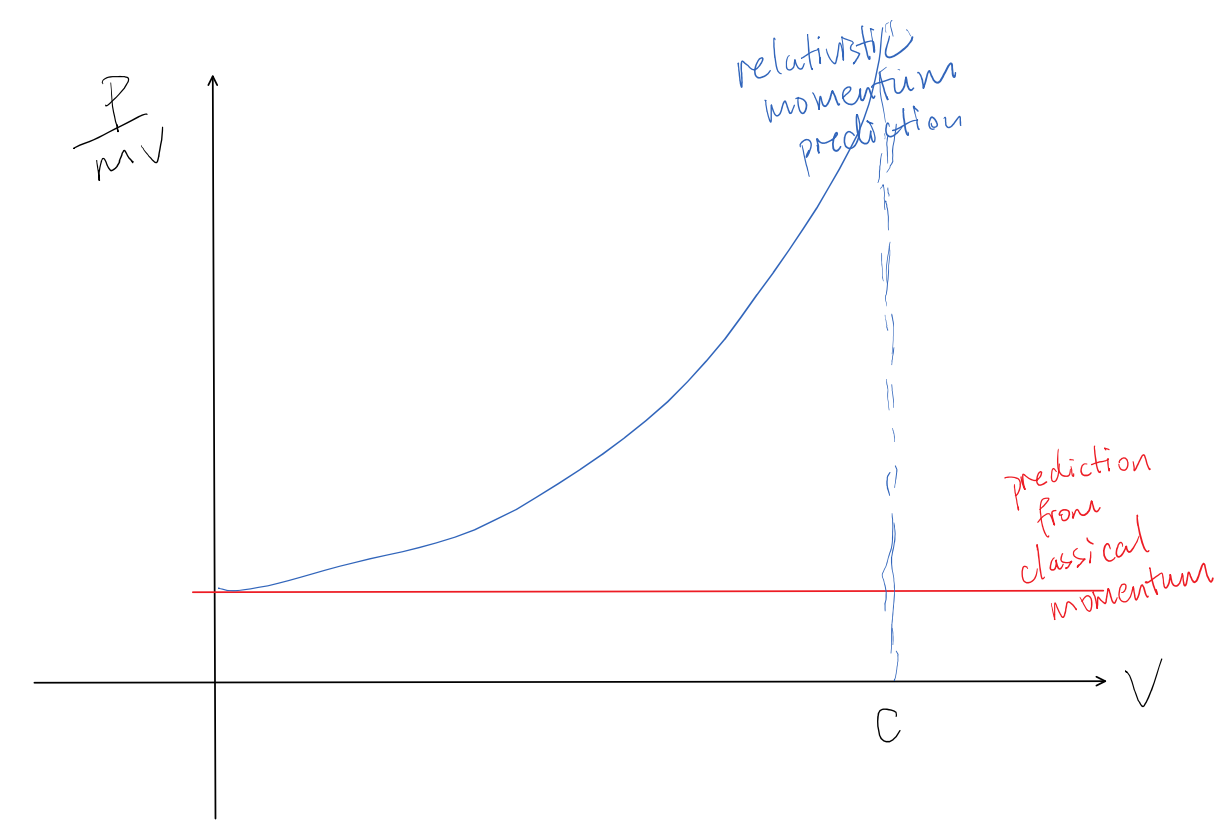
\includegraphics[scale=0.3]{Screenshot (632).png}
\end{center}


\newpage
\textbf{Newton's Second Law}\\
In special relativity, we write $$\vec{F} = \frac{d\vec{p}}{dt} \qquad \qquad \qquad \ \ \ \text{with } \vec{p} = \frac{m\vec{v}}{\sqrt{1-\frac{v^2}{c^2}}}$$

Here we note that, if we have $\vec{v}$ perpendicular to $\vec{F}$, such as the case where the object is moving in a circular motion,  then given that $v = |\vec{v}|$ is constant, $\frac{dv}{dt} = 0$, and hence $\frac{d\gamma}{gt} = 0$, in which case we have the following: $$\vec{F} = \frac{d\vec{p}}{dt} = \frac{d}{dt}(m\vec{v}\gamma) =\gamma m\vec{a}$$

On the other hand, if we have $\vec{v}$ parallel to $\vec{F}$, and hence $v$ is not a constant because the object is accelerated by the force $F$ in the direction of $\vec{v}$. Then we write the following:
$$\vec{F} = \frac{m\vec{a}}{\left(1-\frac{v^2}{c^2}\right)^{3/2}} = \gamma^3 m\vec{a}$$
To summarize, we write the following:
$$\vec{F} = \begin{cases}
\gamma^3 m\vec{a} & \vec{v}\text{ is parallel to } \vec{F} \\ \gamma m\vec{a} & \vec{v}\text{ is perpendicular to } \vec{F} 
\end{cases}$$ 
On another note, if we have $v<<c$, then it is immediate that $1-\frac{v^2}{c^2}\approx 1$, so $\gamma\approx 1$, and we have $\vec{p} = \frac{m\vec{v}}{\sqrt{1-\frac{v^2}{c^2}}}$ tends to $m\vec{v}$, and $\vec{F}$ tends to $m\vec{a}$. \\

\newpage
\textbf{Relativistic Energy}\\
In Classical Newtonian Mechanics, we have $\vec{p} = m\vec{v}$. Suppose we have a box with mass $m$ initially at $x_1$, and being moved to $x_2$ in the positive $x$ direction, with a force $\vec{F}$. When the box is at $x_2$, it has a speed $v_0$. From this setting, we can write the following:
\begin{align*}
\Delta KE = KE_f - KE_i = W = \int_{x_1}^{x_2} Fdx = \int_{x_1}^{x_2} ma\ dx
\tag{1}\end{align*}
Note that, in both Classical Newtonian Mechanics and Special Relativity, we have the followings hold:
$$v=\frac{dx}{dt} \qquad \qquad\qquad a=\frac{dv}{dt}$$
$$\Rightarrow\qquad \frac{dv}{dx} = \frac{dv/dt}{dx/dt} = \frac{a}{v}\qquad \Rightarrow \qquad v\ dv = a\ dx$$
Now we can rewrite equation (1) with the following:
$$\Delta KE = \int_{x_1}^{x_2} ma\ dx = m\int_{0}^{v_0} v\ dv = m\left[\frac{1}{2}v^2\right]^{v_0}_0 = \frac{1}{2}mv_0^2$$

However, in the context of Special Relativity, we have $F = \gamma^3 m a$ when $\vec{F}$ is parallel to $\vec{v}$. Hence we need to rewrite as the following:
\begin{align*}
\Delta KE = W = \int_{x_1}^{x_2} \frac{ma}{(1-v^2/c^2)^{3/2}}\ dx \ \ \ \qquad \text{ with } a\ dx = v\ dv
\end{align*} 
Hence we can write the following:
\begin{align*}
\Delta KE = W &= \int_{0}^{v_0} \frac{mv}{(1-v^2/c^2)^{3/2}}\ dv \\&= \int_{0}^{v_0} \frac{d}{dv}\left(\frac{mc^2}{(1-v^2/c^2)^{1/2}}\right)\ dv\\ &=\left[\frac{mc^2}{(1-v^2/c^2)^{1/2}}\right]_0^{v_0}\\ &= \frac{mc^2}{\sqrt{1-\frac{v_0^2}{c^2}}}-mc^2 
\end{align*}
As a result, in Special Relativity, we write the following:
$$KE = mc^2 \left(\frac{1}{\sqrt{1-v^2/c^2}} - 1\right) = mc^2(\gamma-1)$$

Here we note that, when $v<<c$, we can write the following:
$$\frac{1}{\sqrt{1-\beta^2}}=1+\frac{1}{2}\beta^2 + \frac{3}{8}\beta^4 + \cdots \ \ \ \text{for }\beta<<1$$
$$KE = mc^2\left(1+\frac{1}{2}\left(\frac{v}{c}\right)^2+\frac{3}{8}\left(\frac{v}{c}\right)^4+\cdots -1\right) = \frac{1}{2}mv^2+\frac{3}{8}m\frac{v^4}{c^2}+\cdots $$
where $\frac{3}{8}m\frac{v^4}{c^2}$ and other higher order terms are suppressed when $v<<c$, hence we get $KE = \frac{1}{2}mv^2$ when $v<<c$. \\

In Newtonian Mechanics, the total energy, which is the total potential energy with the total kinetic energy, is conserved. In Special Relativity, the energy that is conserved is the Total Relativistic Energy of an object with rest mass $m$ and speed $v$, defined by the following:
$$E = \frac{mc^2}{\sqrt{1-\frac{v^2}{c^2}}}$$
This obeys the energy conservation in all inertial frames.\\

Notice that, when we have $v=0$, we have the rest energy of the particle given by the following:
$$E = mc^2$$
We say that an object of mass $m$ at rest has a total relativistic energy $E = mc^2$.\\

\newpage
On another note, we have the following holds:

$$E^2 = \frac{m^2c^4}{1-\frac{v^2}{c^2}} \qquad \qquad \qquad p^2 = \frac{m^2v^2}{1-\frac{v^2}{c^2}}$$

$$\Rightarrow E^2-p^2c^2 = \frac{m^2c^4-m^2v^2c^2}{1-\frac{v^2}{c^2}} = \frac{m^2c^4(1-\frac{v^2}{c^2})}{1-\frac{v^2}{c^2}} = m^2c^4$$
Here we conclude the following:
$$E^2 -p^2c^2 = m^2c^4 \qquad\qquad\qquad \text{or}\qquad\qquad\qquad E^2 = p^2c^2 + m^2c^4$$
Here are some consequences of this:\\
A massive particle ($m\neq 0$) at rest
($p=0$) has energy $E = mc^2$. \\
A massless particle ($m=0$) at rest ($p=0$) has energy $E = pc$. \\
Note here, a massless particle, such as a photon, cannot be at rest, in fact, they must move at the speed of light. Moreover, only particles that are massless can move at the speed of light. \\

Note that, in the discussion above, we have $KE =\frac{1}{2}mv^2+\frac{3}{8}m\frac{v^4}{c^2}+\cdots $, where $\frac{1}{2}mv^2$ is the Newtonian kinetic energy contribution, and the $\frac{3}{8}m\frac{v^4}{c^2}$ is the leading relativistic correction. Here we write the following:
$$0.1 = \frac{\frac{3}{8}m\frac{v^4}{c^2}}{\frac{1}{2}mv^2} = \frac{3}{4}\frac{v^2}{c^2} \qquad \Rightarrow \qquad v\approx 0.37c \ \ \ \text{with } \gamma \approx 1.074$$
The mass of an electron is $m_e = 9.11\ee^{-31}$ kg. The relativistic kinetic energy of an electron traveling at $v\approx 0.37c$ is $KE = m_ec^2(\gamma-1) \approx 6.1\ee^{-15}J$. Here $KE = 6.1\ee^{-15}J \approx 37\ee^3\ eV =37\ keV$.\\\\

\begin{defn}
The kinetic energy gained by an electron accelerated from rest across an $1$ Voltage electric potential is $1\ eV = 1.602\ee^{-19}J$
\end{defn}

In particle physics and nuclear physics, we commonly use $eV$, electron volts, to measure energies.
$$keV = 10^3\ eV \qquad \qquad \qquad MeV = 10^6\ eV \qquad \qquad \qquad GeV = 10^9\ eV$$
For electron mass, we write the following:
$$m_e = \frac{E}{c^2} = \frac{9.11\ee^{-31}kg\ c^2}{c^2} = \frac{8.2\ee^{-14}J}{c^2} = 511\ keV/c^2$$


In the following, we will give a experimental verification of the relativistic energy.\\

The Bertozzi Experiment. A generator is used to accelerate electron up to a certain energy, and the energy gained by the electron is controlled by the voltage. The range of the energy gained by the electron ranges from $0.5$ to $15$ MeV. By this setting, the electron with known $KE$, has a speed $v$ measured by the flight time and distance. Then we plot $\frac{KE}{m_ec^2}$ vs. $\frac{v^2}{c^2}$. In classical mechanics, we have $\frac{v^2}{c^2} = \frac{2KE}{m_ec^2}$, as KE approaches $\infty$, $\frac{v^2}{c^2}$ approaches $\infty$. In special relativity, we have $\frac{v^2}{c^2} = 1-\left(\frac{m^ec^2}{KE+m^ec^2}\right)^2$, as KE approaches $\infty$, we have $\frac{v^2}{c^2}$ approaches $1$. The experimental result shows that the curve approaches the horizontal line $1$. \\









\newpage
Suppose there is a mass $m_1$ moving in the $x$ direction to the right with momentum $\vec{p}_1$, and mass $m_2$ moving in the $x$ direction to the left with momentum $\vec{p}_2$. In the center of mass frame (CM), we have $\vec{p}_1 = -\vec{p}_2$. Here we note that the total momentum of the system is given by $\vec{p}_{total} = \vec{p}_1+\vec{p}_2 = 0$, and the total energy is given by the following: 
$$E_{total}^{initial} = E_1^{initial} + E_2^{initial} = \text{ Sum of KE and Rest Energy of the masses} = E_{total}^{final}$$
where $E_{total}^{initial}$ and $E_{total}^{final}$ are the initial and final energy of the system, respectively. $E_1^{initial}$ and $E_2^{initial}$ are the initial total energy of the masses, respectively. Here we can use $E_{total}^{initial}$ to create new particle. Say the two masses are electron and positron, and get only a pion $\pi^0$ at rest after the collision, which as mass $135 MeV/c^2$. That is, the positron and the electron are eliminated by the process of collision.
$$E_{total}^{initial} = E_{e-}+E_{e+} \approx 1\ MeV + KE = E_{total}^{final} = 135\ MeV = m_{\pi^0} c^2$$
without special relativity, we might write the following to find the speed of either the positron or the electron, note here positron and electron have the same masses: 
$$\frac{1}{2}(0.511 MeV/c^2)\cdot v^2 = \frac{1}{2}\cdot (135\ MeV/c^2)\cdot c^2 \qquad \Rightarrow \qquad v = 16\ c$$
which is impossible, hence we need to fix ti by using theory of special relativity:
$$E_e = \frac{m_ec^2}{\sqrt{1-\frac{v^2}{c^2} }} = \frac{1}{2}m_{\pi^0} c^2 \qquad \Rightarrow \qquad v\approx 0.99997 c$$


\hfill\break
\hfill\break
\hfill\break

Example. [Higgs Particle] \\
The mass of the Higgs is around $125\ GeV/c^2$, and Higgs can be created by proton-proton high speed collision. Higgs is very unstable, it has a lifetime around $1\ee^{-22}$ seconds. One possible decay of the Higgs is two photons, which have high energy and can be detected. When decay, we have $E_H = E_{\gamma} + E_{\gamma} = 125\ GeV$, and the photons will go in opposite directions, with $E_{\gamma} = 62.5\ GeV$.  






\newpage
\textbf{Lorentz Transformation for Relativistic Energy and Relativistic Momentum}\\
Suppose we have two frames $S(x,y,z,t)$ and $S'(x',y',z',t')$, where $S'$ is moving at a speed $u$ in the $x$-direction. Suppose there is a particle in frame $S$ moving witha  speed $\vec{v}$, having a relativistic momentum $\vec{p}=(p_x,p_y,p_z)$ and relativistic energy $E$. We denote the corresponding relativistic momentum of the particle in $S'$ as $\vec{p}'=(p'_x,p'_y,p'_z)$, and the relativistic energy of the particle in $S'$ as $E'$.\\

Use the definition of $\vec{p}$ and $E$, together with the velocity Lorentz Transformation, we get:
\begin{align*}
&p'_x = \gamma \left(p_x-\frac{u}{c^2}E\right)
\qquad \qquad  \qquad
p'_y = p_y \qquad \qquad  \qquad
p'_z = p_z \qquad \qquad  \qquad
E' = \gamma(E-up_x)
\end{align*} 
Here we note that: $$c^2(p_x^{'2}+ p_y^{'2}+p_z^{'2})-E^{'2} = c^2(p_x^{2}+ p_y^{2}+p_z^{2})-E^{2} = -m^2c^4$$
such equality is invariant.\\

From the result above, we say that the rest mass of a particle is Lorentz invariant. The rest mass is a well defined characteristic of a particle in Special Relativity.\\

That is, we know that, for massless particle $m=0$ in one frame, then the particle is massless $m=0$ in all inertial frames. That is, when $m=0 \iff v=c$ in one frame, then $m=0 \iff v'=c$ in all frames.\\


\newpage
\textbf{Twin Paradox}\\
Suppose Ryan is going away from the Earth to a far away star with a speed $u = \frac{99}{101}c$, and Ethan stays on Earth. Let $S$ be the Earth's rest frame, and let $S'$ be Ryan's rest frame.\\

From Ethan's point of view, Ryan's outbound trip takes $\Delta t = 101\ years$ to reach the star that is $99\ lightyears$ away, the distance is measured by Ethan on Earth, and he believes that, due to time-dilation effect, Ryan will say the outbound trip only takes $\Delta t' = 20\ years$ to reach the star. \\

However, from Ryan's point of view, Ryan sees Ethan is moving away from him, as his outbound trip only takes $20\ years$, he will say that Ethan's clock only takes $3.96\ years$. Here we reach a paradox.\\

Let Event A be the event that Ryan arrives at the star. In $S'$, Event A happens at $t' = 20\ years$. By Lorentz Transformation, we can write the following:
$$t' = \gamma ( t - \frac{u}{c^2}x) = \frac{101}{20}(t-\frac{99}{101}\frac{x}{c}) = 20\ years$$
\begin{align*}
t = \frac{99}{101}\frac{x}{c} + 3.96\ years
\tag{1}\end{align*}
Notice here equation (1) is a straight line in $(\frac{x}{c},t)$ space-time diagram, which is the line called the Line of Simultaneity. That is, any point on this line in $S$ corresponds to $t'=20\ years $ in $S'$. \\
\begin{center}
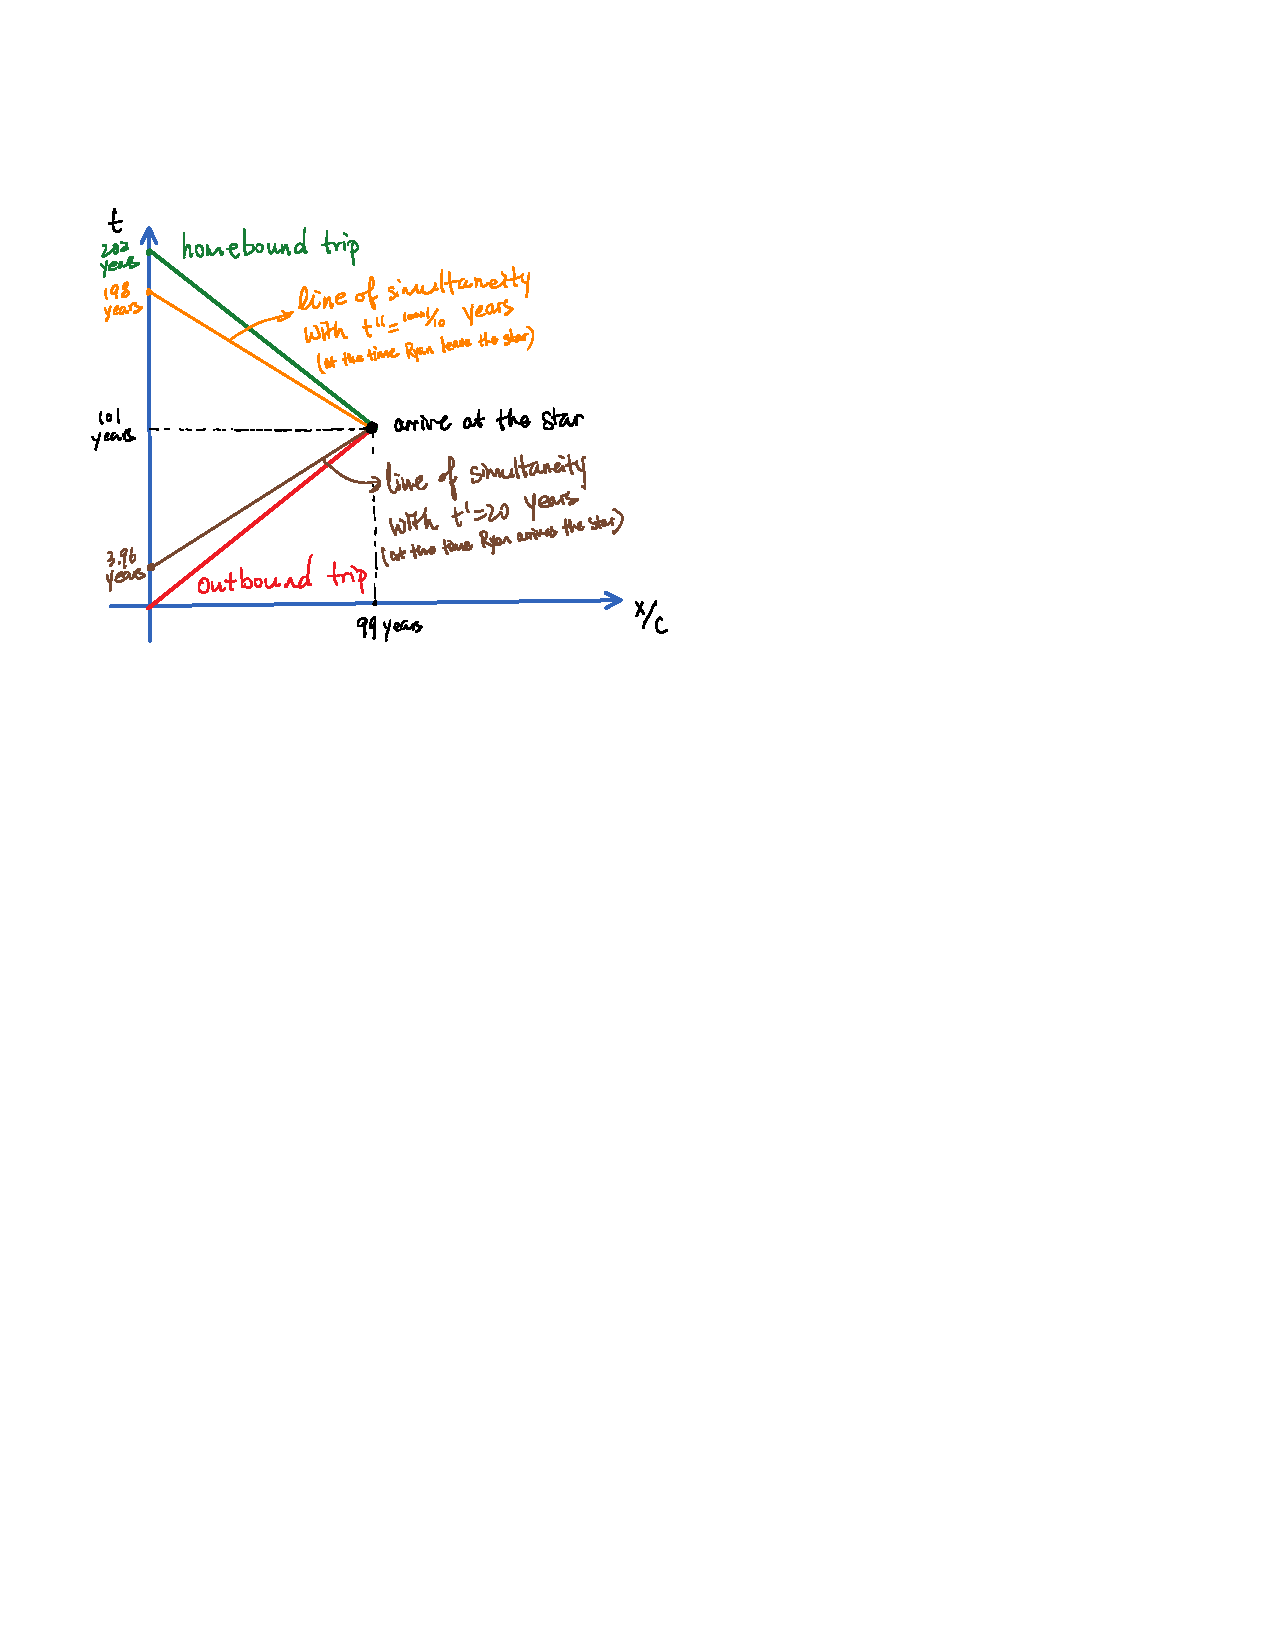
\includegraphics[scale=1]{lineOfSimultaneity.pdf}\\
\end{center}
From this picture, we know that, from the point of view of Ryan's outbound rest frame $S'$, the two events described as the following are simultaneous:\\
(1) Ryan got 20 years older since departure from Earth.\\
(2) Ethan getting 3.96 years older since Ryan departed.\\

Notice there is no paradox here, because at different points in space, two observers may not agree on simultaneity. \\

Now consider Ryan's homebound rest frame, denoted as $S''$ with time $t''$ in this frame. We can write the following by Lorentz Transformation:
$$t'' = \gamma(t+\frac{u}{c^2}x) = \frac{101}{20}(t+\frac{99}{101}\frac{x}{c})$$
When Ryan arrives at the star, we have $t = 101\ years$, and $x/c = 99\ years$. Hence we can write the following: 
$$t''= \frac{101}{20}(101\ years + \frac{99}{101}101\ years) = \frac{10001}{10}\ years$$
So the line of simultaneity of Ryan's departure from the star is given by the following: 
$$\frac{10001}{10}\ years = \frac{101}{20}( t+ \frac{99}{101}\frac{x}{c})$$
$$t = \frac{-99}{101}\frac{x}{c} + \frac{20002}{101}\ years$$
In $S$, when $x/c = 0$, the line of simultaneity gives $t= \frac{20002}{101}\ years \approx 198\ years$. Here, we claim the following:\\

\textit{The moment Ryan changes from outbound to homebound, on the star, the lines of simultaneity jump. That is, the intersection of the lines of simultaneity jump from 3.96 years to 198 years. Of course, no clocks on Earth suddenly jumps.}\\

The fact that Ryan jumps from frame to frame is what breaks the symmetry of the problem here. \\

Suppose light signals are sent back to the Earth by Ryan every 5 years in Ryan's rest frame. These frequency of these light signals are translated to around every 50 years in Ethan's rest frame when Ryan's is moving away from the Earth, and translated to around every 0.5 years in Ethan's rest frame when Ryan is going towards the Earth.\\

Lights emitted from the source moving away from the receiver arrive less frequently to the receiver. The light signals emitted from the source moving towards the receiver arrive more frequently to the receiver.\\

\newpage
\textbf{Light}\\
Suppose a train moving in the x-direction with a speed $u$, and a light is sent from the train. A person at rest on Earth sees the train coming towards him and sees the light, and claim that the light has energy $E'$. Now the train stops moving, the same light source from the train emits a light again, and a person at rest on Earth sees such light, and claim that such light has energy $E$. Here we will have $E' = p'c$, and $E=pc$, with $E>E'$, and $p>p'$.\\

Light is an EM wave, which has wavelength $\lambda$, and frequency $\nu$, and we have the following: $$c = \lambda\nu$$
where frequency is defined to be the number of wavetops go by per second, and wavelength is defined to be the length between two wavetops. For short wavelength, the light has high frequency. For long wavelength, the light has low frequency.\\ 

Light is also a particle, called the photon. Photon is massless, always travels at a speed $c$, and has no electric charge. Photon carries energy given by the following:
$$E = h\nu$$
where $h$ is the Planck's Constant, and $\nu$ is the frequency of light.\\

Light from a source that is moving away from the observer should have less energy and lower frequency $\mu$, in which case we called the light is redshifted. Light from a source that is moving towards the observer should have more energy and higher frequency, in which case we say the light is blueshifted. \\

\textbf{Derivation of Special Relativity Doppler Formula}\\
Suppose there are two inertial frames $S$ and $S'$, $S'$ is moving at a speed $u$ in the $x$-direction carrying a light source emitting a light. In $S$, the light has frequency $\nu$, energy $E = h\nu$ and momentum $p = \frac{E}{c}$, moving in the $x$ direction towards an observer at rest in $S$. In $S'$, the same light has frequency $\nu'$, energy $E' = h\nu'$, and momentum $p' = \frac{E'}{c}$. \\

By Lorentz Transformation, we can write the following:
$$E'=\gamma(E-up_x) = \gamma\left(E-u\frac{E}{c}\right) = \frac{E(1-u/c)}{\sqrt{(1-u/c)(1+u/c)}} = E\sqrt{\frac{1-u/c}{1+u/c}}$$
Similarly, we can get the following:
$\nu' = \nu \sqrt{\frac{1-u/c}{1+u/c}}$, which is the Relativistic Doppler Formula for light source approaching the observer given $u$ is positive. If light source is moving away, we take $u$ be negative. 

\newpage
\textbf{Derivation of the Lorentz Transformation}\\
Here we will derive the Lorentz Transformation from the two postulates of Special Relativity.\\

Recall that Einstein's postulates for Special Relativity is given by the following:\\
(1) \textbf{Principle of Relativity}. The Laws of Physics are the same in every inertial frames.\\
(2) \textbf{Speed of Light is Constant}. The speed of light in vacuum is the same in all inertial frames and it is independent of the motion of the light source.\\

Suppose we have two inertial frames $S(x,t)$ and $S'(x',t')$, where $S'$ is moving with a speed $u$ in the positive $x$-direction. Suppose there is a light signal emitted from $x=0$ at $t= 0$ in the positive $x$-direction. In $S$, we can write $x = ct$ to indicate the position of the light signal in $S$. Also, in $S'$, we can also write $x' = ct'$ to indicate the position of the light in signal $S'$. Hence we can write the following:
$$x - ct = 0 \qquad\qquad\qquad\qquad x'-ct' = 0$$
So it must be that $x,t$ are related to $x',t'$ such that $x-ct = 0 \iff x'-ct' =0$. Notice there must be a linear relationship between $x,t$ and $x',t'$ because straight lines with constant speed in $S$ must be mapped to straight lines with constant speed in $S'$ as physics must be the same in all inertial frames. Then there must exists some constant $A \neq 0$ such that the following hold:
\begin{align*}
x' - ct' = A (x-ct) \tag{1}
\end{align*}

Similarly, for light signal emitted in the negative $x$-direction in $S$, we can write the following:
$$x = -ct \qquad\qquad\qquad\qquad x' = -ct'$$
Rearranging we get the following:
$$x+ct = 0 \qquad\qquad\qquad\qquad x'+ct' = 0$$
Then $\exists\ B \neq 0$ such that the following holds: \begin{align*}
x'+ct'=B(x+ct)  \tag{2}
\end{align*}
Adding equation (1) and (2), we get the following:
$$(x'-ct') + (x' + ct') = A(x-ct) + B(x+ct)$$
rearranging we get the following:
$$x' = \frac{A+B}{2}x - \frac{A-B}{2}ct$$
Let $a,b$ be the following:
$$a = \frac{A+B}{2} \qquad\qquad\qquad\qquad b = \frac{A-B}{2}$$
Then we can write the following:
\begin{align*}
x' = ax-bct\tag{3}
\end{align*}
Subtract equation (2) from (1), we can write the following:
$$(x'-ct')-(x'+ct') = A(x-ct) - B(x+ct)$$
rearranging we get the following:
$$ct' = \frac{A+B}{2}ct - \frac{A-B}{2}x$$
with $a,b$ defined above, we get the following:
\begin{align*}
t' = at-b\frac{x}{c} \tag{4}
\end{align*}
Here we note that, we use first postulate to justify that $(x,t)$ and $(x',t')$ must be linearly related. And we use second postulate to derive the equations (3) and (4) above.
\newpage

For the origin at $x'=0$ in $S'$, such origin is at $x = ut$ in frame $S$. On the other hand, we have $x' = ax-bct$ by equation (3), hence we can write the following:
$$x' = ax-bct \qquad \Rightarrow \qquad 0 = ax - bct \qquad\Rightarrow \qquad x = \frac{b}{a}ct \qquad\Rightarrow\qquad b = \frac{u}{c}a$$
So now we can rewrite equation (3) and (4) as the following:
\begin{align*}
x' = a(x-ut) \qquad\qquad\qquad\qquad t'=a(t-\frac{u}{c^2}x) \tag{5}
\end{align*}
In the following we will find $a$. Suppose we have inertial frames $S(x,t)$ and $S'(x',t')$, $S'$ is moving at a speed $u$ in the positive $x$-direction. Suppose we have two scenarios:\\ 
\begin{enumerate}
\item A measure stick at rest in $S'$ is measured to have length $L_0$, extend from $0$ to $x'_0$, and a person at rest in $S$ observe such measure stick has length $L$, extend from $0$ to $x_0$.
\item Now we put the same stick at rest in $S$, and observe that the length of the stick is $L_0$, extend from $0$ to $x$, and a person at rest in $S'$ observe the rest stick in $S$ has a length $L'$, extend from $0$ to $x'$.
\end{enumerate}
By the first postulate, we must have $L' = L$, since the two scenarios are physically equivalent. \\
In scenario 1, we take a snapshot at $t=0$, then we can write the following:
$$x_0' = a\left(x_0 - u \cdot 0\right) = ax_0 \qquad \Rightarrow \qquad L_0 = aL$$
In scenario 2, we take a snapshot at $t'=0$, then we can write the following:
$$0 = t' = a\left(t - \frac{u}{c^2}x\right) \qquad\Rightarrow\qquad t = \frac{u}{c^2}x$$
$$x' = a\left(x-ut\right) = a\left(x-u\cdot \frac{u}{c^2}x\right) = a\left(1-\frac{u^2}{c^2}\right)x$$
so we can write the following:
$$L' = L = a\left(1-\frac{u^2}{c^2}\right)L_0$$
while we have $L_0 = aL$, we can write the following:
$$L = a\left(1-\frac{u^2}{c^2}\right) a L$$
rearranging we get the following:
$$\gamma\coloneqq a = \frac{1}{\sqrt{1-\frac{u^2}{c^2}}}$$
And hence we can rewrite equation (3) and equation (4) as the following:
$$x' = \gamma\left(x-ut\right) \qquad\qquad\qquad\qquad t' = \gamma\left(t- \frac{u}{c^2}x\right)$$
This completes the derivation of the Lorentz Transformation.

\newpage
\section{\color{red} Thermodynamics}
When you rub your hands together, your make mechanical energy using muscles, which create frictions and generates heat, then the temperature of your hands increases.\\

Heat is a form of energy transfer.\\

Temperature is a measure of an object's cold or hot. More precisely, temperature is the average kinetic energy of the molecules of an object.\\

We will first need to understand the concept of thermal equilibrium. Consider taking your temperature using a thermometers. Your body comes to a thermal equilibrium with the thermometers so that the thermometers can measure your temperature. Note also that the tip of the thermometer is metal. This is because metal is a thermal conductor.\\

Thermal conductors are materials that allows heat to exchange.\\
Thermal insulator are materials that allows only little or no heat exchange.\\

Ideal insulator allows no heat exchange. \\


\textbf{The Zero-th Law of Thermodynamics}\\
For systems A, B and C. If A is in thermal equilibrium with C, and B is in thermal equilibrium with C, then A and B are in thermal equilibrium.\\

The two systems are in thermal equilibrium if and only if they have the same temperature. Let $T_A$ denote the temperature of $A$, Let $T_B$ denote the temperature of $B$, and let $T_C$ denote the temperature of $C$. Then we have $T_A = T_C$, $T_B=T_C$ implies $T_A = T_B$.\\

Assuming 1 atmosphere pressure. For Fahrenheit scale, water freezes at $30^\circ F$, boils at $212^\circ F$, and body temperature is around $100^\circ F$. For Celsius scale, water freezes at $0^\circ C$, boils at $100^\circ C$, and body temperature is around $37^\circ F$. For Kelvin scale, which is the absolute scale, water freezes at $273K$, boils at $373K$, and body temperature is around $310K$. \\

Here we can write: 
$$T_F = \frac{9}{5}T_C + 32^\circ F$$
$$T_K = T_C + 273.15K$$
where $T_F = T_K = T_C$ represents the temperature in Kelvin, Celsius, and Fahrenheit scale, respectively.\\

$T= 0K$ defines the absolute zero, in which case the system has a minimal average Kinetic Energy.\\

\newpage
\textbf{Thermal Expansion}\\

When we add heat to an object, typically, the average distance between neighboring atoms increases, that is, the material expands.\\

For linear expansion, suppose we have an object originally has length $L_0$ at temperature $T_0$, now apply a temperature difference $\Delta T$, the length of the object linearly expands to $L_0 + \Delta L$, then we can write the following relationship:
$$\Delta L = \alpha L_0\Delta T$$
where $\alpha$ is some constant depending on the type of the object, with a unit $1/^\circ C$ or $1/K$, depending on the unit of temperature.

\begin{center}
\begin{tabular}{|c|c|c|c|}
\hline 
Materials & Linear expansion coeff. $\alpha$& Area expansion coeff. & Volume expansion coeff. $\beta$\\
\hline
Aluminum & $2.4\ee^{-5}$ & $4.8\ee^{-5}$ & $7.2\ee^{-5}$\\ \hline
Copper & $1.7\ee^{-5}$ & $3.4\ee^{-5}$ & $5.1\ee^{-5}$\\ \hline
Steel & $1.2\ee^{-5}$ & $2.4\ee^{-5}$ & $3.6\ee^{-5}$\\ \hline
Brass & $2.0\ee^{-5}$ & $4.0\ee^{-5}$ & $6.0\ee^{-5}$\\ \hline
\end{tabular}
\end{center}

With $\beta = 3\alpha$, here we have the followings:
$$\Delta L =\alpha L_0 \Delta T$$
$$\Delta A = 2\alpha A_0 \Delta T$$
$$\Delta V = \beta V_0 \Delta T$$
Notice here, we can write the following:
$$V = L^3 \qquad\Rightarrow\qquad dV = 3L^2dL = 3L^2(\alpha LdT) = 3L^3\alpha dT = \beta V dT$$
The idea also applies for area expansion coefficient $2\alpha$.\\

There is an exception of such thermal expansion. The material water. When water freezes to ice, its volume increases. Also, for temperature greater than around 4$^\circ C$, water expands linearly with $\beta \approx 2\ee^{-4} \frac{1}{{}^\circ C}$ just as described for solids when heat is added. However, when the temperature is between $0^\circ C$ and $4^\circ C$, the water expands when heat is taken out of it. As a result, we know that water is most dense at around $4^\circ C$.

\newpage
\textbf{Heat and Phase Transitions}\\

In thermal dynamics, there are mainly two kinds of variables, the Intensive variable and the Extensive variable. If we divide the system into halves, and the variable does not change, then such variable is called Intensive variable, otherwise, if the variable does change, then such variable is called an Extensive variable.\\

Examples:\\
Suppose we have a box of gas, it has volume $V$, temperature $T$, and air pressure $p$. \\Here $V$ is extensive, $T$ and $p$ are intensive, when we divide the box to halves.\\

Suppose we have a stretched wire, which has length $L$, temperature $T$, and tension $\sigma$. \\Here $L$ is extensive, $T$ and $\sigma$ are intensive when we cut the wire by half.\\

Given two systems with different temperature, the amount of heat that is exchange between two system depends on the temperature difference and masses of the two system. 
$$\Delta Q = m c_p \Delta T$$
where $\Delta Q$ is the amount of heat exchange, $m$ is the mass, $c_p$ is the specific heat of the material, and $\Delta T$ is the temperature difference. The unit of $c_p$ is $\frac{J}{kg\ K}$ or $\frac{J}{kg\ {}^\circ C}$, depending on the unit of $\Delta T$. $c_p$ represents the amount of energy it takes to raise the temperature of $1\ kg$ of the object by $1K$.\\

Whenever the temperature of the two system is different, then heat must flows from the system with higher temperature to the system with lower temperature.\\

Example:\\
For ice, $c_p = 2.114 \frac{kJ}{kg\, K}$, for liquid water, $c_p = 4.1813 \frac{kJ}{kg\, K}$, and for water in gas form, $c_p = 2.01 \frac{kJ}{kg\, K}$.\\

$1$ Calorie is defined to be the amount of heat required to raise the temperature of $1g$ of water from $14.5^\circ C$ to $15.5^\circ C$. $1\ cal = 4.186\ J$ and $1\ kcal = 4186\ J$.\\

Note here, the amount of exchanged heat is not proportional to the change in temperature when the material is under phase change.\\

First Order Phase Transition requires energy to take place, such energy is called the Latent Heat. For example, when water goes from ice form to liquid form, it requires $334\frac{kJ}{kg}$, called the heat of fusion. When water goes from liquid form to gas form, it requires $2256\frac{kJ}{kg}$, called the heat of evaporation.\\

Second Order Phase Transition does not require latent heat to transform from one phase to another. For water, there is a critical point at atmospheric pressure 217.75 atm, with temperature at 374$^\circ C$. After this point, there is no distinction between gas and liquid. \\

Example:\\
Ferromagnets has the property that, below a critical temperature $T_{curie}$, the magnet is magnetic, and above $T_{curie}$, the magnet is not magnetic. Below the $T_{curie}$, the magnet is said to be in ordered phase, and said to be in disordered phase above the $T_{curie}$. At $T_{curie}$, the system become scale invariant.\\

At the critical point, $T_{curie}$ for ferromagnets and $374^\circ C$ at $217.75$ atm for water, water and ferromagnets are described by the same model.
\newpage
\textbf{Fundamental Postulate of Statistical Mechanics}\\

If equal probability for each particle to be on the left hand side or right hand side of the box, what are the possible arrangements?\\

The fundamental postulate of statistical mechanics states that each possible microscopic arrangement is equally likely.\\

Macrostates:\\Macroscopic configurations of the system is equally likely. The macrostate of our example is that there are "two particles on the left and two on the right," but without worrying about the detail of which two particles on the left.

$$P(\C) = \frac{\text{number of microstate in }\C}{\text{total number of microstates}}$$
 
Note that the sum of all probabilities is one.

$$\sum_{\C} P(\C) = 1$$

Microstates:\\In microstate, we keep track of each of the possible arrangements of that that give the macrostate. This takes into the detail of which particular particle is on the left or right.\\

The number of ways that can we pick $k$ objects out of a set of $n$ identical ones. without sorting or ordering, and no putting back:
$$\begin{pmatrix}
n\\k
\end{pmatrix} = \frac{n!}{k!(n-k)!}$$


Example:\\
Say we have 10 red socks and 6 blue socks. Randomly pick one, then there are 16 total microstates, the probability of getting red is $10/16 = 5/8$, and the probability of picking blue is $6/16=3/8$.\\ 

The probability of picking two identical socks is given by the following:\\

In such case, we have three macrostates, two blues, two reds, and one blue one red. 
$$\text{total number of microstates} = \frac{16!}{2!(16-2)!} = 120$$
$$\text{total number of choosing two red socks out of the ten reds} = \frac{10!}{2!8!} = 45$$
$$\text{total number of choosing two blues socks out of the six blues} = \frac{6!}{2!4!} = 15$$
$$\text{total number of choosing one red and one blue} = 10\cdot 6 = 60$$
\newpage\textbf{Heat Conduction}
When heat is added to a system, one of the two things might happen:
\begin{enumerate}
\item Temperature changes, $\Delta Q = mc_p\Delta T$, where $c_p$ is the specific heat, and $m$ is the mass.
\item The temperature remains constant while the system undergoes first order phase transition, $\Delta Q = m L$, where $L$ is the latent heat, $m$ is the mass. 
\end{enumerate}

Different materials have different thermal conductivity $k$. The unit for conductivity is $\frac{W}{m\,K}$.\\

The flow of heat is defined to be the following:

$$H = \frac{dQ}{dt}$$
with unit $J/s = W$. 
Now suppose we have a cold object with temperature $T_C$ and a hot object with temperature $T_H$. Connect the two objects with some material $A$, the flow of heat between the object depends on the type of the material $A$, the cross-sectional area of the material $A$, the temperature difference between the two objects, and the length of the connection $A$, given by the following equation:
$$H = \frac{dQ}{dt} = kA\frac{T_H - T_C}{L}$$
where $H$ describes the heat flow, $k$ is the thermal conductivity, here $k$ has a unit $\frac{W}{m\,K}$\\

Example:\\
Silver has conductivity of $406 \frac{W}{m\,K}$, wood has conductivity of $0.04\sim 0.1 \frac{W}{m\,K}$\\
Hence we say that wood is not a good thermal conductor.\\

Suppose we have an object with length $L$, constant cross-sectional area $A$, temperature on the left with $T_H$ and temperature on the right with $T_C$. We want to investigate $H$ as a function of position $x$. We expect $H=\frac{dQ}{dt}>0$ because heat flows from left to right as time passes by, but $\frac{dT}{dx}<0$ because temperature decreases as we go from left to right.
$$H = \frac{dQ}{dt} = -kA \frac{dT}{dx}$$
heat flows faster with larger temperature gradient.

\newpage
\textbf{Heat Radiation}\\
All objects at all temperatures emit energy in the form of electromagnetic radiation. The larger the object's surface area $A$, the larger the emitted energy, and the larger the temperature $T$ of the object, the larger the emitted energy, the emitted energy is given in the form of heat, by the following :
$$H = \frac{dQ}{dt} = eA\sigma T^4$$
where $\sigma$ is the Stefan-Boltzmann's constant: 
$$\sigma = 5.67\ee^{-8} \frac{W}{m^2K^4}$$
and $e$ is the emissivity of the object with $0 < e \leq 1$.\\
$$e = \begin{cases} e=1 & \text{Blackbody}\\
e\approx 1 & \text{Black surface}\\
e\approx 0.3 & \text{Smooth metal surface}\\ e\approx 0 & \text{Ideal reflector}    \end{cases}$$
when an object has $0< e<1$, we say the object is a Graybody. Blackbody is the ideal absorbor, or radiator. \\

When an object is in thermal equilibrium with its surroundings, it must absorb exactly as much heat as it is emitting. Hence we can write the following:
$$|H_{absorb}| = |H_{emit}| = eA \sigma T^4$$
Heat absorption has the same equation as heat radiation when the object is in thermal equilibrium. Here $T$ is the temperature of the object and the environment. But when the object is not in thermal equilibrium with the surrounding, and the surrounding has temperature $T_2$ and the object has temperature $T_1$, then we write the following:
$$|H_{emit} |=eA\sigma T_1^4 \qquad\qquad\qquad\qquad |H_{absorb}| = eA\sigma T_2^4 $$
Intensity is defined to be the radiation per surface area of an object. For blackbody, which has a emissivity of $1$, it has an intensity given by the following:
$$I = \sigma T^4$$
For other object, the intensity is given by:
$$I = e\sigma T^4$$
\hfill\break
\hfill\break
\hfill\break

Electromagnetic wave propagate in vaccune at the speed of light $c = 2.99792\ee^8\ m/s$. It has a wavelength $\lambda$ and a frequency $\nu$, and we write the following:
$$c = \lambda \nu$$
Here we note that a shorter wavelength implies a higher frequency. Visible light is the electromagnetic wave with wavelength in the range between $\sim 380\,nm$ and $\sim 760\,nm$. The lower end is the red light and the upper end is the blue light. Below the lower end, we have infrared, and beyond the upper end, we have ultraviolet.  A blackbody emits radiation at all wavelength, but it emits the most radiation at a wavelength given by 
$$\lambda_{MAX}(T) = \frac{2.898\ee^{-3} Km}{T}$$
such is known as the Wien's Displacement Law.\\

\newpage
In the following we want to investigate how the intensity vary with the wavelength. \\

The intensity of blackbody radiation depends on the wavelength of the radiation $\lambda$ and the temperature $T$, here we write the following:
$$I_T(\lambda)$$
Given that $T_H >T_L$, we have $I_{T_H}(\lambda) > I_{T_L}(\lambda)$ for all $\lambda$. Hence we say blackbody radiation curves never cross. There is higher intensity at any wavelength for the hotter object. Also, for $T_H > T_L$, we have $\lambda_{MAX}(T_H) < \lambda_{MAX}(T_L)$, so the maximum value of the intensity shifts to shorter wavelengths as $T$ increases, such is described by the Wien's Displacement Law:
$$\lambda_{MAX}(T) = \frac{2.898\ee^{-3} Km}{T}$$
The intensity curves are described by the Plank's Formula:
$$I_{T}(\lambda) = \frac{2\pi hc^2}{\lambda^5} \frac{1}{e^{hc/(\lambda k T)} - 1}$$
where $T$ has a unit $K$, $k$ is the Boltzmann's constant with $k = 1.38\ee^{-23} J/K$, $h$ is the Plank's constant with $h = 6.63\ee^{-34}J\cdot s$. Note that, for a given $T$, as $\lambda$ tends to infinity, we have $I_T(\lambda)$ tends to $0$. When $\lambda$ tends to $0$, we also have $I_T(\lambda)$ tends to $0$. For a given $T$, we have $\max\{I_T(\lambda) \mid \lambda >0 \}$ given by $\lambda_{MAX}(T) = \frac{2.898\ee^{-3} Km}{T}$. For a given $T$, the total intensity added up over all wavelengths is given by the following:
$$I_{total}(T) = \int_{0}^\infty I_T(\lambda) d\lambda = \sigma T^4$$
which is exactly the total intensity for a blackbody. The Stefan Boltzmann Law states that the total area under the Plank curve is given by $\sigma T^4$. \\

Note here, the Plank's formula involves the Plan's constant $h$, which implies there is something related to the quantum physics in this formula. Before Plank (1900), Rayleigh used classical physics to describe blackbody radiation, he found that the intensity of a blackbody radiation is given by the Rayleigh-Jean's Formula:
$$I_T^{RJ}(\lambda) = \frac{2\pi L}{\lambda^4} kT$$
Note here, the Rayleigh-Jean's Formula has some problems:
\begin{enumerate}
\item It does not match experiment or observations, such as the Sun.
\item Intensity diverges when wavelength is tiny
\item Infinite amount of radiation at short wavelengths
\item Area under the Rayleigh-Jean's curve diverges.
\end{enumerate}
So the Rayleigh-Jean's Formula must not be correct. The problem here was Rayleigh-Jean 's Formula assumed that radiation can be emitted in arbitrarily small quantities. While Plank's assumed that there must be a smallest unit of emitted energy, that is, the radiation is emitted in quanta of $E = h\nu$ where $\nu$ is the frequency of the light, and $h$ is the Plank's Constant. Here we can also write:
$$E = \frac{hc}{\lambda}$$
And here, the energy of the quanta $E$ are photons. From Special Relativity, we know that $p= E/c$, and $E= pc$ for any massless particle. Here we can conclude that the wavelength, or equivalently the frequency, of the EM wave determines the energy it carries. \\

\begin{center}
\includegraphics[scale=0.5]{intensityCurves.pdf}
\end{center}

\newpage
\textbf{Statistical Mechanics}\\

The ideal gas law states that:
$$pV = nRT$$
where $n$ is the measure of number of molecules in gas in moles. Let $N$ be the number of molecules, we have:
$n = \frac{N}{N_A}$
where $N_A$ is the Avogadro Number $N_A = 6.02\ee^{23} \frac{\text{molecules}}{\text{mol}}$. $1$ mol is the amount of substance that contains as many molecules as there are in twelve grams of Carbon-12. \\

Example: The volumes of a typical classroom is around $10\,m \times 20\,m \times 40\,m = 8000\,m^3$. The atmospheric pressure is $1\,atm$, and typical room temperature is around $20^\circ C = 293\, K$. Here we have $n = \frac{pV}{RT} = 3\ee^6\,mol$, and $N = nN_A = 10^{30}$ air molecules in a classroom. \\

One might code up the trajectories of many many non-interacting molecules using classical mechanics, but probably not for $10^{30}$ molecules. Instead, we can describe the gas using thermaldynamic variables, such as extensive volume, intensive pressure and temperature, and variables like heat, work, entropy, etc.. The statistical mechanics uses probability to connect between the microscopic level, the trajectory of each gas molecule, and the core of thermaldynamics. That is, statistical mechanics describe the average behaviors of microscopics using thermaldynamic variables.\\

Example:\\
In gas model, the average kinetic energy for the translational motion of the molecules is given by:
$$\bar{E}_{traslational} = \frac{3}{2}kT$$
where $k$ is the Boltzmann's Constant. \\

\newpage
\textbf{Boltzmann Distribution}\\
Consider discrete energy levels $E_i$ in an atom, each level has a probability $p_i$ that satisfies:
\begin{enumerate}
\item $0\leq p_i \leq 1$
\item $\sum_{s=1}^\infty p_s = 1$
\item There is an expectation value that describe the average energy level. $<E> = \sum_{s=1}^\infty E_s\cdot p_s$
\end{enumerate} 
Such a system with discrete energy levels, one might ask what is the probability of the system to be found in a state with energy $E_s$? If the system is in thermal equilibrium with temperature $T$, in Kelvin, then the probability of finding the system in energy state $E_s$ is given by the following:
$$\Power(s) = \frac{1}{Z}e^{-\beta E_s}$$
where $\beta = \frac{1}{k\cdot T}$, $k$ is the Boltzmann's Constant, and $Z$ is the partition function, determined by the normalization condition such that $\sum_s \Power(s) = 1$, so we have: 
$$Z = \sum_{s} e^{-\beta E_s}$$

\hfill\break
Example:\\
The Hydrogen atom has infinitely many discrete energy states $E_1,E_2,\cdots$, with $E_1$ the lowest state called the ground state, $E_2$ being the first excited state, $E_3$ being the second excited state, etc. Here $E_2 - E_1 = 10.2 \,eV$. Imaging we have a big cloud of hydrogen atoms, and say such big cloud is at the surface of the sun, with temperature around $T= 5800\,K$. The probability of finding hydrogen atom in the ground state is $\Power (s_1) = \frac{1}{Z} e^{-\beta E_1}$, and the probability of finding hydrogen atom in the first excited state is $\Power(s_2) = \frac{1}{Z} e^{-\beta E_2}$. For the relative probability between $\Power(s_1)$ and $\Power(s_2)$, we can write the following:
$$\frac{\Power(s_2)}{\Power(s_1)}=\frac{e^{-\beta E_2}}{e^{-\beta E_1}} = e^{-(E_2-E_1)/(kT)}$$
where $k = 1.38\ee^{-23}\, J/K = 8.62\ee^{-5}\,eV/K$, with $T = 5800\,K$, $\Rightarrow kT = 0.5\,eV$. 
Hence:
$$\frac{\Power(s_2)}{\Power(s_1)}= e^{-(E_2-E_1)/(kT)} \approx e^{-20} \approx 10^{-9}$$
This tells us that for every one billion hydrogen atom at the surface of the Sun, one is the first excited state, and the rest of them is in the ground state, the probability of finding hydrogen atom at higher excited state will be even much smaller. However, there are actually 4 out of $10^9$ hydrogen atoms are in the first excited state. This is caused by the degeneracies in the hydrogen atom in this model: There are multiple states that has the same energy. The degeneracy for $E_1$ is $2$, for $E_2$ is $8$, and for $E_3$ is $18$. So here we need to adjust the Boltzmann Distribution using the following:
$$Z = \sum_{s} e^{-\beta E_s} = 2e^{-\beta E_1} + 8e_{-\beta E_2} + 18e^{-\beta E_3} + \cdots \qquad\qquad \qquad \Power(s) = \frac{1}{Z}d(E_s) e^{-\beta E_s}$$
with $d(E_s)$ being the degeneracy of energy state $E_s$. Now we can rewrite:
$$\frac{\Power(E_2)}{\Power(E_1)} = \frac{d(E_2) e^{-\beta E_2}}{d(E_1)e^{-\beta E_1}} = 4e^{-\beta (E_2-E_1)} \approx 4 \ee^{-9}$$
So $4$ in a billion of hydrogen atoms are int eh first excited states on the surface of the Sun. This is what can be actually observed. We observe that, at even higher excited state, the probability is even more suppressed, and when we have higher temperature, it becomes easier to see an atom at higher excited state. That is, higher temperature implies more atoms being excited, and lower temperature implies fewer atoms being excited.\\

Example:\\
For hydrogen gas at room temperature $T \approx 300\,K$, $kT \approx 0.026\,eV$, here we can write:
$$\frac{\Power(\text{first excited state})}{\Power(\text{ground state})} \approx 10^{-171}$$
and here we see that for a gas at room temperature, we can ignore internal excitation of the atomic energy levels.\\

For a gas, molecules move around with different velocities in different directions. An atom, or molecule, of the gas with speed $v$ in some direction $\hat{v}$ has kinetic energy given by $E_v = \frac{1}{2}mv^2$, where $m$ being the mass of the atom, or molecule, of the gas. The probability of finding such atom with speed $v$ in a gas in thermal equilibrium with temperature $T$ involves studying continuous probability distribution because the quantity $E_v$ is continuous. 


\newpage

\textbf{Probability distribution}\\
The probability of finding at particle at exactly position $x_0$ is zero. However, one can ask the probability of finding a particle lies in small position interval $dx$, given by:
$$p(x_0)dx = \text{area under the probability curve on }dx$$
The probability of finding the particle at any position $x$ is one. In such case we say the probability distribution is normalized, and requires the following holds:
$$\int_{-\infty}^\infty p(x) dx = 1$$
\\

Example.\\
Suppose at position $x$, the particle has some property $f(x)$. (For example, $f(x)$ can represent the potential energy of the particle at $x$). The average of such property (average of potential energy for example), is given by the following:
$$<f> = \int_{-\infty}^\infty f(x)p(x)\, dx$$
This is the continuous version of the probability of discrete levels discussed above.\\


\hfill\break
Example.\\ 
Suppose we have a particle whose probability of appearing at position $x$ is encoded by the function $p(x)$, then the average position of the particle is given by:
$$<x> = \int_{-\infty}^\infty x p(x) dx$$
And squared average position of the particle is given by:
$$<x^2> = \int_{-\infty}^\infty x^2 p(x) = dx$$
Standard deviation, a measure of the spread of measurements around the average value is given by:
$$\sigma = \sqrt{<x^2> - <x>^2}$$


\hfill\break\hfill\break
\textbf{Gaussian Distribution}, or the Normal Distribution, is encoded by the function: 
$$p(x) = c\cdot e^{-\frac{(x-a)^2}{2\sigma^2}}$$
where $c$ is the normalization constant dependent on $a$ and $\sigma$. The constant $a$ characterizes the center of the distribution, and the constant $\sigma$ characterizes the spread, and the shape, of the distribution. 

\newpage
\textbf{Maxwell-Boltzmann Distribution}\\
We want to answer the question: What is the probability of finding a particle with speed $v$ in gas at temperature $T$. Here we note that $KE = \frac{1}{2}mv^2 = E_v$, and the Boltzmann Distribution also applies when there is a continuum of possible states:
$$\Power(v) = C \cdot d(E_v) \cdot e^{-\beta E_v}$$
where we have:
$$e^{-\beta E_v} = e^{\frac{mv^2}{2kT}}$$
The degeneracy is the "numbers" of the $\vec{v}$ that gives rises to $|\vec{v}| = v$ for given $v$. If this is a one dimensional problem, then there are two options for the direction of $\vec{v}$, hence in one dimension, we have $d_{1d} (v) = 2$. If the problem is two dimensional, we might draw a circle with radius $v$, and any vector $\vec{v}$ tipping at the circumference of the circle has length $v$, so we can write $d_{2d}(v)  = 2\pi v$. For three dimensional problem, we can draw a sphere with radius $v$, and the surface are gives the measure of the number of state for $v$, that is, we have $d_{3d} (v) = 4\pi v^2$. One can calculate the normalization constant $C = (\frac{m}{2\pi kT})^{3/2}$. So now we can write the following:
$$\Power(v) = \left(\frac{m}{2\pi kT}\right)^{3/2}\cdot 4\pi v^2 \cdot e^{-\frac{mv^2}{2kT}}$$
This is called the Maxwell-Boltzmann Distribution. Here $\Power(v)\,dv$ gives us the probability of finding the particle with speed in neighborhood $dv$ around $v$. We also observe that as $v$ tends to $0$, we have $\Power(v)$ tends to $0$, and as $v$ tends to $\infty$, we have $\Power(v)$ tends to $0$. $\Power(v)$ is also temperature dependent, when $T$ is higher, $\Power(v)$ peaks at a greater $v$, but the peak is lower, and the shape of the cure is more normal. Here the the speed $v$ of the peak of the distribution is called the most probable speed at given temperature $T$. When the gas grows hotter, the most probable speed increases.\\


Note here, the most probable speed at a given temperature is in general, not equal to the average speed of the particles in such given temperature. The root mean square speed is also not equal to the most probable speed, nor the average speed, in general. 
$$\text{Average Speed} = \left<v\right> = \int_{0}^\infty v\cdot \Power(v)\, dv$$
$$\text{Root mean square speed} = v_{rms} = \sqrt{\left<v^2\right>} = \sqrt{\int_0^\infty v^2\cdot \Power(v)dv} = \sqrt{\frac{3kT}{m}}$$
Note that we integrate from $0$ to infinity because the speed of a particle is non-negative. Also note here we have $\left<v^2\right> = \frac{3kT}{m}$. And note that we also have the average kinetic energy of the particles in given temperature $T$ to be the following:
$$\left<KE\right> = \left<\frac{1}{2}mv^2\right> = \int_{0}^\infty \frac{1}{2}mv^2\Power(v)\, dv = \frac{1}{2}m\left<v^2\right> = \frac{3}{2}kT$$
Here we see that the temperature of the gas directly reflects the average kinetic energy of the system. 



\newpage
\textbf{Convection}\\
\textbf{Example}: Ideal gas law: $pV = nRT$, when $p$ is fixed, $n$ is fixed, an increase in $I$ implies an increase in volume, so the density of gas decreases, hence hot gas will always goes up. This is also the key point of an air balloon, as the hot air, or liquid, moves, the heat is transported. Due to this, heater and radiator are usually put on the floor instead of on the ceiling. \\

There are two types of convection:
\begin{enumerate}
\item Forced convection. A pump that circulate the gas or liquid that transports heat.
\item  Natural convection. No pump.
\end{enumerate} 

Human heart is an example of forced convection. \\
Air rises due to lower density is an example of natural convection.



\newpage
For a monatomic gas molecule, the three transnational degree of freedom are the only ones. For diatomic molecules, there are three degree of freedom for transnational motion, two rotational degree of freedom, and two vibration degree of freedom. \\

\textbf{Equipartition Theorem}\\
Each available degree of freedom contributes $\frac{1}{2}kT$ to the average energy. \\

For monatomic gas, there are three degrees of freedom, hence $<E> = 3\cdot \frac{1}{2}kT$. \\From Maxwell-Boltzmann distribution, $<KE>=<E> = \frac{3}{2}kT$.\\

For diatomic gas, there are three transnational degrees of freedom available at all energies at all temperatures. In Quantum mechanics, energy levels of rotations and vibrations are discrete, or quantized, and it takes a certain minimal energy to access these degrees of freedom. It takes less energy to excite rotations than vibration in diatomic molecules. 



\newpage
\textbf{Work}\\

\textbf{Molar Heat Capacity}. For a fixed volume, $dQ = n\,C_v\,dT$. When heat is added to the system, temperature goes up, and when heat is removed from the system, temperature goes down.\\

For sign convention. Heat is added to the system, we say $Q>0$. Heat is removed from the system, we say $Q<0$. System does work on surroundings, we say work $W>0$. Surroundings does work on the system, we say work $W<0$.\\

To calculate the work done by a gas system, suppose gas is in a container that has a changeable volume $V$. A piston with cross-sectional area $A$ is attached to this container. The piston can move up and down with distance $dx$, then the volume of the container changes by $dV = A\,dx$. Note that for pressure $p$, we have $p = F/A$. The work done by the gas to the piston is given by $dW = F\,dx = p\,Adx = p\,dV$. If the volume of the system changes from $V_i$ to $V_f$, then the work done by the gas is given by the following:
$$W= \int_{V_i}^{V_f} dW = \int_{V_i}^{V_f} p\, dV$$
Note here $p$ may not be constant in the process, so in general, $p$ cannot be take out from the integral.\\

\textbf{pV-Diagram} is a diagram that gives pressure as a function of volume.\\

Note here work is path dependent.\\


Suppose heat $Q$ is added to the system, and work $W$ is done by the system. As total energy of the system must conserve, the change in the interval energy of the system is given by: 
$$\Delta U = Q-W$$
The internal energy of the system only depends on the state of the system, not how it got to that state. That is, $\Delta U$ is path independent. The \textbf{cyclic process} is the process where the final state (volume and pressure) is equal to the initial state. In a cyclic process, we have $\Delta U = 0 = Q-W \Rightarrow Q = W$, that is, work $W$ is done by the system, and the same amount of heat $Q$ is need to be added to the system. \\

\textbf{First Law of Thermodynamics} states that $Q - W = \Delta U$, and $\Delta U$ is path independent. In another words, we have $dQ -  dW = dU$.\\

\begin{center}
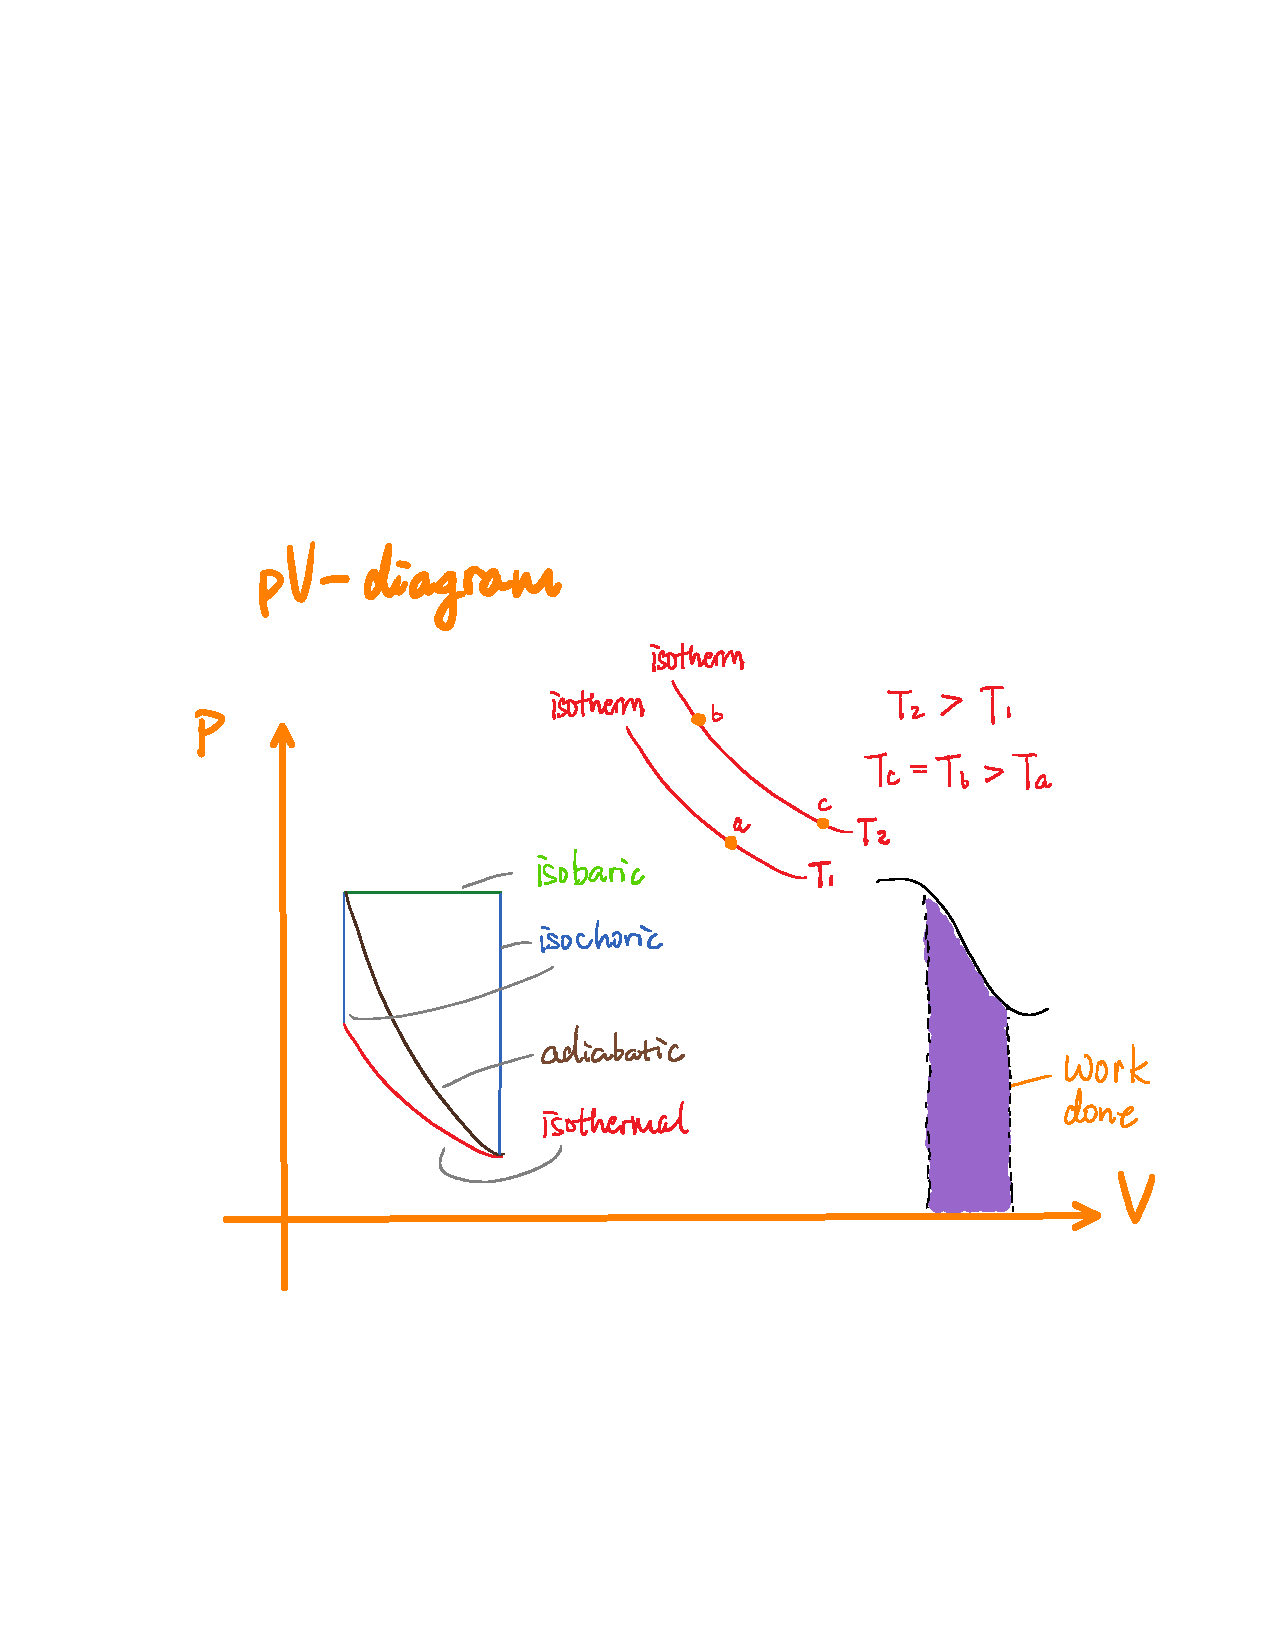
\includegraphics[scale=0.8]{pVdiagram.pdf}
\end{center}


\newpage
\textbf{Thermodynamic Processes}\\

\textbf{Isochoric Process} - Constant volume, no work done by the system, $\Delta U = Q$.\\
\textbf{Isobaric Process} - Constant pressure. $W = p(V_f - V_i)$.\\
\textbf{Isothermal Process} - Constant temperature. $p_iV_i = p_fV_f$ for ideal gas.\\
\textbf{Adiabatic Process} - No heat exchange during the process, that is, $Q= 0$, so $\Delta U = -W$.\\
\textbf{Cyclic Process} - Initial state is equal to the final state.\\
\textbf{Isolated System} - $Q = W = 0$, and we have $\Delta U = 0$ by the First Law of Thermodynamics. \\

In general, isochoric process and isothermal process have non zero $Q$, $W$, and $\Delta U$. 
For ideal gas in isothermal process, $pV$ is a constant as temperature of the system is a constant, and we have:
$$W = nRT\ln(V_f/V_i) = nRT\ln(p_f/p_i)$$
Typically, adiabatic process happens very fast, so there is not time to loose heat.\\


\hfill\break\hfill\break\hfill\break

\textbf{Internal Energy}\\
$\Delta U = U_f - U_i$, where we have:
$$U = \sum_{\text{All molecules in the system}} (E_{kinetic} + E_{potential})$$
The total internal energy of the system does not matter in general, it is change in internal energy that matters. Average kinetic energy is reflected in temperature $T$ as we discussed previously.\\

For any ideal gas, the internal energy depends only on the temperature of the system.\\

Free expansion of an ideal gas in an isolated system. \\
Suppose we have a container isolated from the environment. The gas in the container are all at the bottom, the top of the container has no gas, the two spaces are separated by a barrier. Suppose the bottom of the container that contains gas has volume $V_i$ and pressure $p_i$. Now we remove the barrier, the volume of the container that contains gas become $V_f$ and pressure becomes $p_f$. For isolated system, we have $Q= W = 0$. By First Law of Thermodynamics, this implies $\Delta U = Q - W =0$. Since $U$ depends only on $T$ in an ideal gas, then we must have $T_f = T_i$, so free expansion of an ideal gas is an isothermal process, and ideal gas law gives us $p_iV_i= p_fV_f$. To conclude: For ideal gas, in free expansion process, $T$ is constant, with $\Delta U = 0$.\\


For non-ideal gas, there is interaction among gas molecules. There is an attractive force between the molecules. When gas expands, the average distance between the molecules increases, so the potential energy in the system increases because the force between the molecules is attractive. Suppose further the system is isolated, then we have $\Delta U = 0$, and here we have $U$ being the sum of potential energy and kinetic energy of the molecules, so we know that the average kinetic energy of the molecules must decrease as the potential energy of the molecules increases. Here it follows that $T$ decreases as average kinetic energy decreases. So here we know that, for non-ideal gas, even thought there is no change in internal energy, the temperature of the system can still change.\\

\newpage
\textbf{Molar Heat Capacity}\\
When one have constant volume, $dQ = n\,C_v\,dT$, or if we have constant pressure $dQ = n\,C_p\,dT$.
Rearranging, we get the followings:
$$C_v = \frac{1}{n}\left(\frac{dQ}{dT}\right)_{\text{fixed volume}} \qquad\qquad\qquad C_v = \frac{1}{n}\left(\frac{dQ}{dT}\right)_{\text{fixed pressure}}$$
For monatomic gas, we have $C_v = \frac{3}{2}R$, and for diatomic gas, we have $C_v = \frac{5}{2}R$ where $R = 8.31 J/(mol\,K)$. For all ideal gas, we have: $$C_p = C_v+R$$
 
\newpage
\textbf{Adiabatic Process}\\

By definition, adiabatic process is a process that has no heat exchange, that is, we have $Q = 0$. For ideal gas, we have $pV = nRT$. For isothermal process, we have $pV$ being constant. For isochoric process, we have $T/p$ being constant. And for isobaric process, we have $T/V$ being constant. For adiabatic process, which we will derive in the following, we have $TV^{\gamma-1}$ being constant, where $\gamma = \frac{C_p}{C_v}$ as $C_p$ and $C_v$ are molar heat capacity for constant pressure and constant volume, respectively. Alternatively, we can write $pV^\gamma$ being constant. Note here we have $C_p = C_v+R$ for an ideal gas, so we have $\gamma = \frac{C_p}{C_v}  = 1+ \frac{R}{C_p} >1$. So we know that, in the pV-diagram, the adiabatic curves are steeper than those of isothermal process.\\

In the following, we will derive $TV^{\gamma-1}$ being constant, for an ideal gas undergoing an adiabatic process. Consider an infinitesimal    adiabatic process, where $dQ = 0$. By the First Law of Thermodynamics, we have $dU = dQ - dW = -dW$, where $dW = p\,dV$, and $dU$ is path independent. For an ideal gas, the internal energy depends only on $T$, so $dU \propto dT$. In our adiabatic process, the temperature change is $T_f - T_i = dT$. \\

Since $dU$ is path independent, we have $dU_{a\to b} = dU_{a\to c} + dU_{c \to b}$, where $a \to c$ is an isochoric process, and $c \to b$ is an isothermal process. By the First Law of Thermodynamic, we have $dU_{a \to c} = dQ_{a \to c} - dW_{a \to c}$ where $dW_{a \to c} = 0$, hence we have $dU_{a \to c} = nC_v dT$. On the other hand, since isothermal process has no change in internal energy, then we know that $dU_{c \to b} = 0$. That is, we can write $dU_{a \to b} = dU_{a\to c} = nC_v dT$. Here we can write 
\begin{align}
-dW = dU = -pdV = nC_v dT \tag{1}
\end{align}
Since $pV = nRT$ for ideal gas, so we have $p = \frac{nRT}{V}$, here we can rewrite equation (1) to get the following:
\begin{align*}
-\frac{nRT}{V}dV = nC^v dT \qquad\Rightarrow\qquad \frac{dT}{T} = -\frac{R}{C_v}\frac{dV}{V} \tag{2}
\end{align*}
Using $R = C_p - C_v$ for ideal gas, we get $R = C_p - C_v \Rightarrow \frac{R}{C_v} = \frac{C_p-C_v}{C_v} = \gamma-1$.  Rewrite equation (2) with such, we get:
\begin{align*}
\frac{dT}{T} =(1-\gamma) \frac{dV}{V} \tag{3}
\end{align*}
We integrate both sides, and get the following:
$$\int \frac{dT}{T} = (1-\gamma) \int \frac{dV}{V} \qquad\Rightarrow\qquad \ln(T) = (1-\gamma) \ln(V)+K$$
for some constant $K$. Rearranging we get our final result:
$$TV^{\gamma-1} = e^{K'}$$
for some constant $K'$, this shows that $TV^{\gamma-1}$ is a constant. Note how each steop of the derivation is broken down into parts, where we use the First Law of Thermodynamics, the ideal gas law, and down to different process, etc. 


\newpage
\textbf{Otto Cycle}\\

Otto cycle is a model of a gasoline engine.\\
\begin{center}
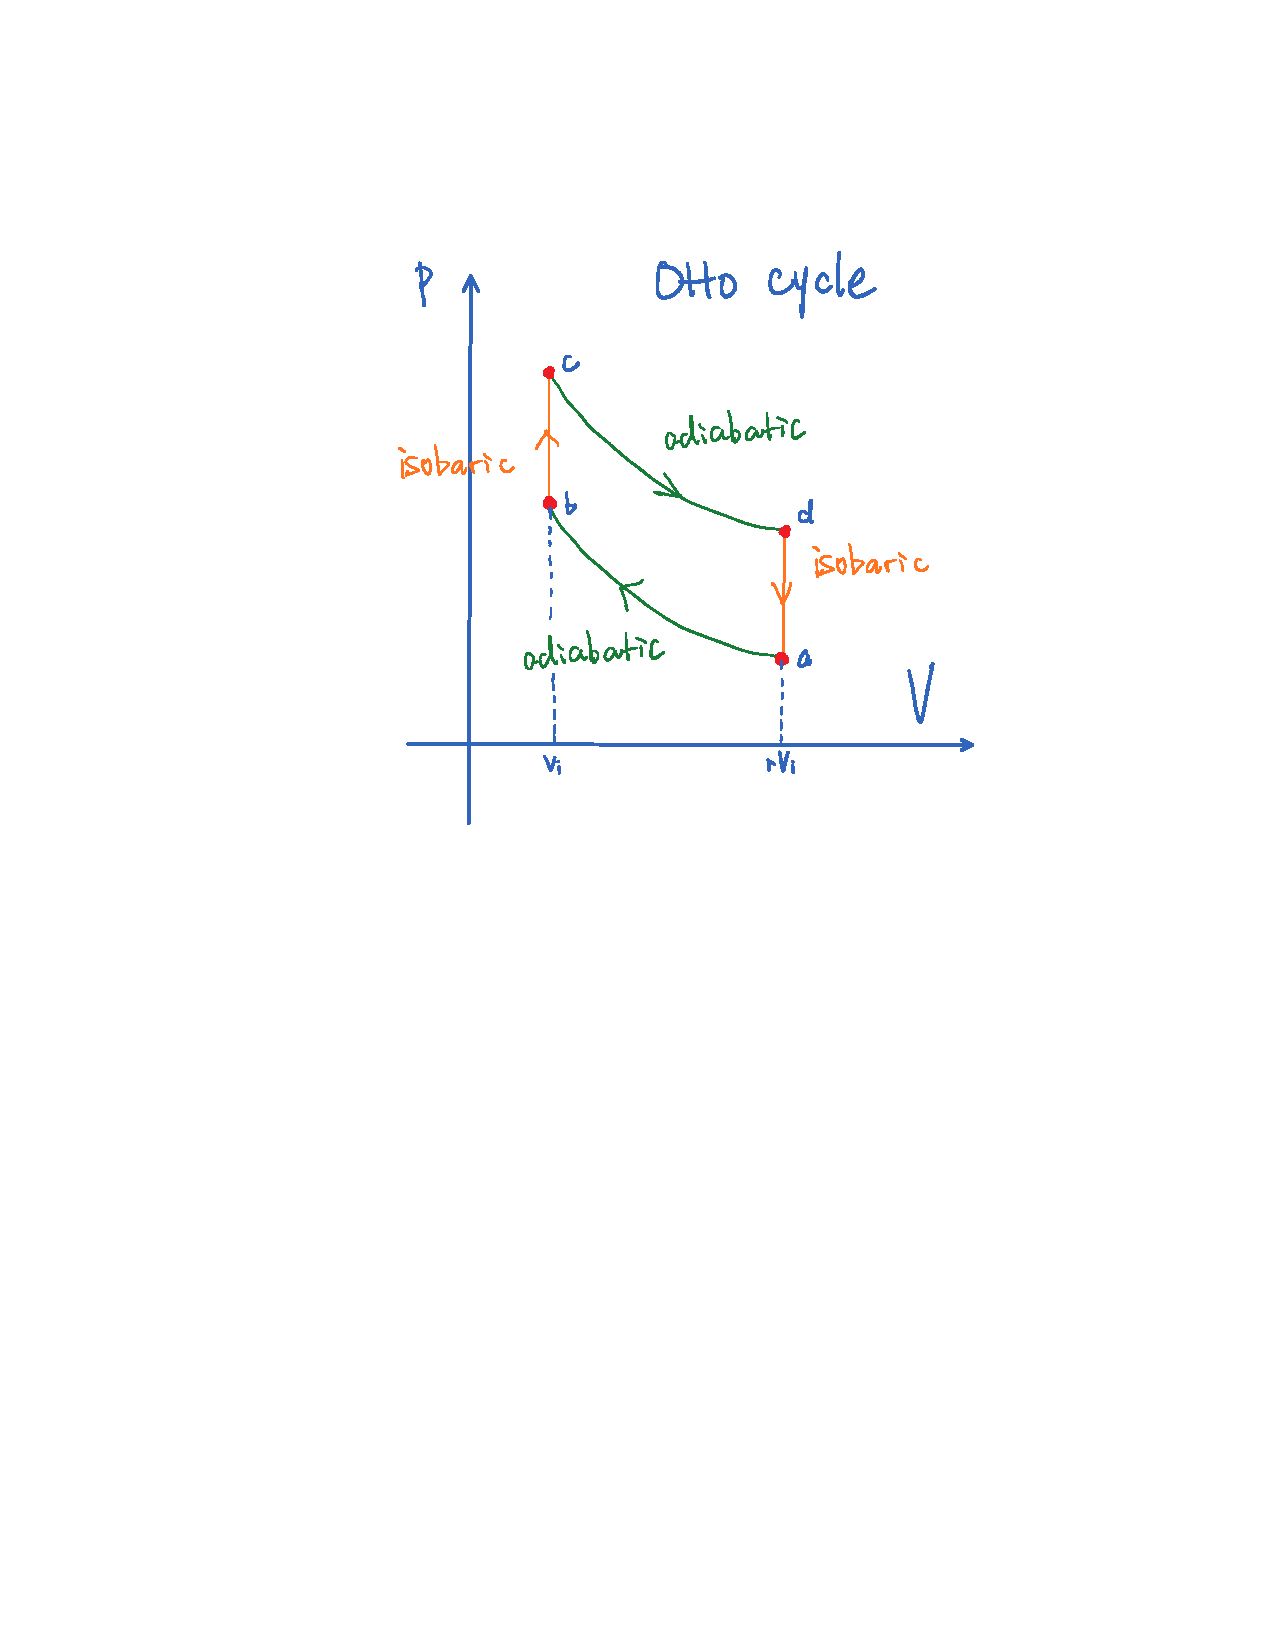
\includegraphics[scale=0.8]{ottoCycle.pdf}
\end{center}

Suppose in the adiabatic process, the volume expands from $V$ to $rV$, then in the following, we will derive the efficiency of the Otto cycle to be $e = 1-\frac{1}{r^{\gamma-1}}$, with $\gamma = \frac{C_p}{C_v}$ for an ideal gas.\\

In order to calculate efficiency, we define efficiency to be $e = 1 + \frac{Q_C}{Q_H}$, where $Q_H$ is the heat get into the system, and $Q_C$ is the heat goes out of the system.\\

Note here we have $Q_{c \to d} = Q_{a\to b}  = 0$ because they are adiabatic process. In isochoric process, we have $V$ being constant, and hence for temperature,we have $T_c>T_b$, and $T_d > T_a$. Also note that, the work done $W_{d\to a} = W_{b \to c} = 0$ because they are isochoric processes.\\

For isochoric processes, by First Law of Thermodynamics, we know that $\Delta U = Q = nC_v\Delta T$, hence we have $Q_H = Q_{b \to c} = nC_v(T_c - T_b) > 0$, and $Q_C = Q_{d \to a} = nC_v(T_a - T_d) < 0$. Now we can write:
\begin{align}
e = 1+\frac{Q_C}{Q_H} = 1 + \frac{T_a - T_d}{T_c - T_b}\tag{1}
\end{align}
We need to relate the temperature to volume. In Adiabatic process, we know that $TV^{\gamma-1}$ is a constant. Here $a \to b$ is adiabatic, then $T_a V_a^{\gamma	-1} = T_b V_b^{\gamma-1}$, hence $T_b = T_a (\frac{V_a}{V_b})^{\gamma-1}$, where $V_a = rV$, and $V_b = V$. Then we can rewrite $T_b = T_a (\frac{rV}{V})^{\gamma-1} = T_a r^{\gamma-1}$. From $c \to d$, we get $T_c V_c^{\gamma-1} = T_dV_d^{\gamma-1}$, with similar argument, since $V_d = rV$ and $V_c = V$, then we get $T_c = r^{\gamma-1} T_d$.  Rewriting equation (1), we get the following:
$$e = 1 + \frac{T_a - T_d}{r^{\gamma-1} T_d - r^{\gamma-1} T_a} = 1+ \frac{1}{-r^{\gamma-1}} = 1- \frac{1}{r^{\gamma-1}}$$

\newpage
\textbf{Refrigerators}\\

Heat engines take heat from hot reservoir with high temperature $T_H$ and produce work. There is always wasted energy in such process, and those wasted energy is dumped into a cold reservoir with low temperature $T_C$. That is, heat enters the system from hot reservoir, denoted as $Q_H>0$, heat leaves the system to cold reservoir, denoted as $Q_C < 0$, and work is done in between, denoted as $W>0$. A refrigerator is an engine that run in reverse. For refrigerator, heat is removed from the cold region and enters the system, denoted as $Q_C >0$, the surroundings also do work on the system, denoted as $W<0$, and heat leaves the system as part of the cooling process, denoted as $Q_H <0$. Note here this is a process that runs in cycle, so that the refrigerator can keep the cold area cold. Here we have $\Delta U = 0$, by the First Law of Thermodynamics, we have $W = Q = Q_H + Q_C$. Here we can write $-|W| = -|Q_H| + |Q_C|$, rearranging we can write:
$$|Q_H| = |W| + |Q_C|$$
The efficient for a refrigerator is defined differently than for a heat engine, because we want to do the least amount of work to remove the most heat from the cold region. The efficiency of a refrigerator is called the coefficient of performance, defined as the following:
$$K \coloneqq \frac{|Q_C|}{|W|} = \frac{|Q_C|}{|Q_H|- |Q_C|}$$
Here we note that $K$ needs not be a number between zero and one, it is a number between zero and infinity. Note here we must put work to the system in order to tale heat from cold regions to hot regions.\\

\begin{center}
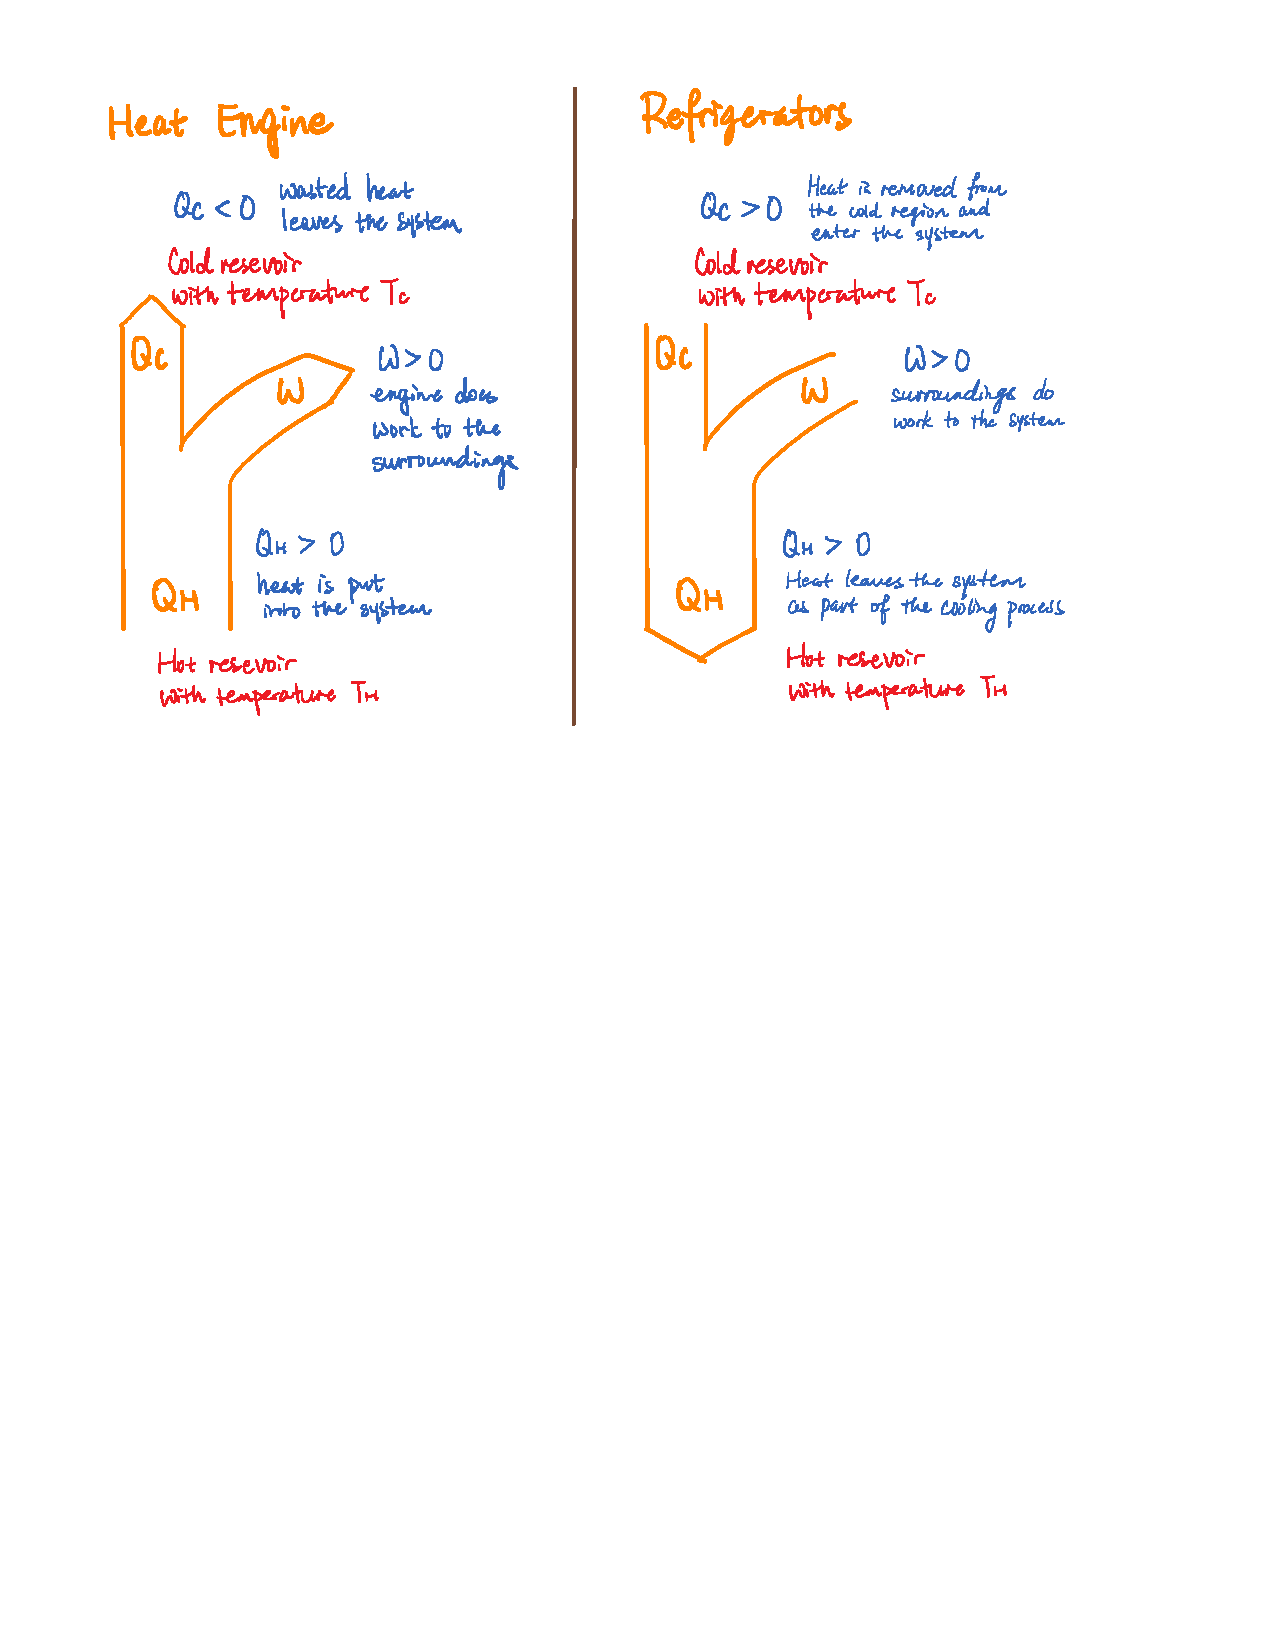
\includegraphics[scale=0.8]{engines.pdf}
\end{center}


\newpage
\textbf{Second Law of Thermodynamics}\\

Heat flows spontaneously from hot to cold, not the other way around. To make heat flow from a colder to a hotter object always requires work. That is, in a refrigerator, we have $W\neq 0$. \\

The Second Law of Thermodynamics can be stated in two ways, here is one of the two ways: \textit{It is impossible for any process to have its sole result the transfer of heat from a cooler to a hotter body.} Such statement is called the "refrigerator version," or the Clausius' Statement.\\

Consider a book sliding across the floor. Microscopicly, moving book has mechanical energy due to organized, coordinated motion of the molecules, and those mechanical energy is transferred into heat and internal energy of the floor and book via friction, here heat and internal energy are represented by KE and PE associated with random motion of the molecules. Here we see that organized motion of mechanical energy is converted into disorganized motion of heat. While it is impossible to have the other way around, such process, going from organized motion to disorganized motion, is called the Irreversible Process. Other examples of irreversible process includes gas flowing from a region of high pressure to one of low pressure, or mixing gas or liquids together. \\

The Second Law of thermodynamics expresses the "one way" aspects of thermodynamic processes, going from organized to disorganized. \\

The other way of stating the Second Law of Thermodynamics is that \textit{it is impossible for any system to undergo a process in which it absorbs heat from a reservoir at a single temperature and converts the heat completely into mechanical work, with the system ending in the same state as it begins.} Such statement is the "engine version," or the Kelvin-Plank Statement. \\

In general, the refrigerator version of the Second Law of Thermodynamics suggests that there is no workless refrigerator, and the engine version of the Second Law of Thermodynamics suggests that there is no 100$\%$ efficient engine. The two statements are equivalent, one implies the other. 

In the following we will show that the two statements of the Second Law of Thermodynamics described above are equivalent. We denote the engine version of the Second Law of Thermodynamics as $\mathcal{B}$, and the refrigerator version as $\mathcal{A}$. To show that $\mathcal{B}$ implies $\mathcal{A}$, we proceed by contradiction. Suppose $\mathcal{A}$ does not hold, then there exists a workless refrigerator. Such refrigerator takes $|Q_C|$ from cold region $T_C$ to $|Q_H|$ in hot region $T_H$, with $|Q_H| = |Q_C|$. Consider an ordinary heat engine that takes $|Q'_H|$ from $T_H$ to $|Q_C|$ in $T_C$ and produce some work $W>0$. Combining the two processes to get a heat engine which has a net production $|Q'_H|$ producing $W$, it does not have wasted energy because $|Q_C|$ can be converted back to $|Q_H|$ in $T_H$ by the workless refrigerator. Here we get a 100$\%$ engine, with $W = |Q'_H|$, hence we reach a contradiction. So we know that $\mathcal{B}$ implies $\mathcal{A}$. \\
\begin{center}
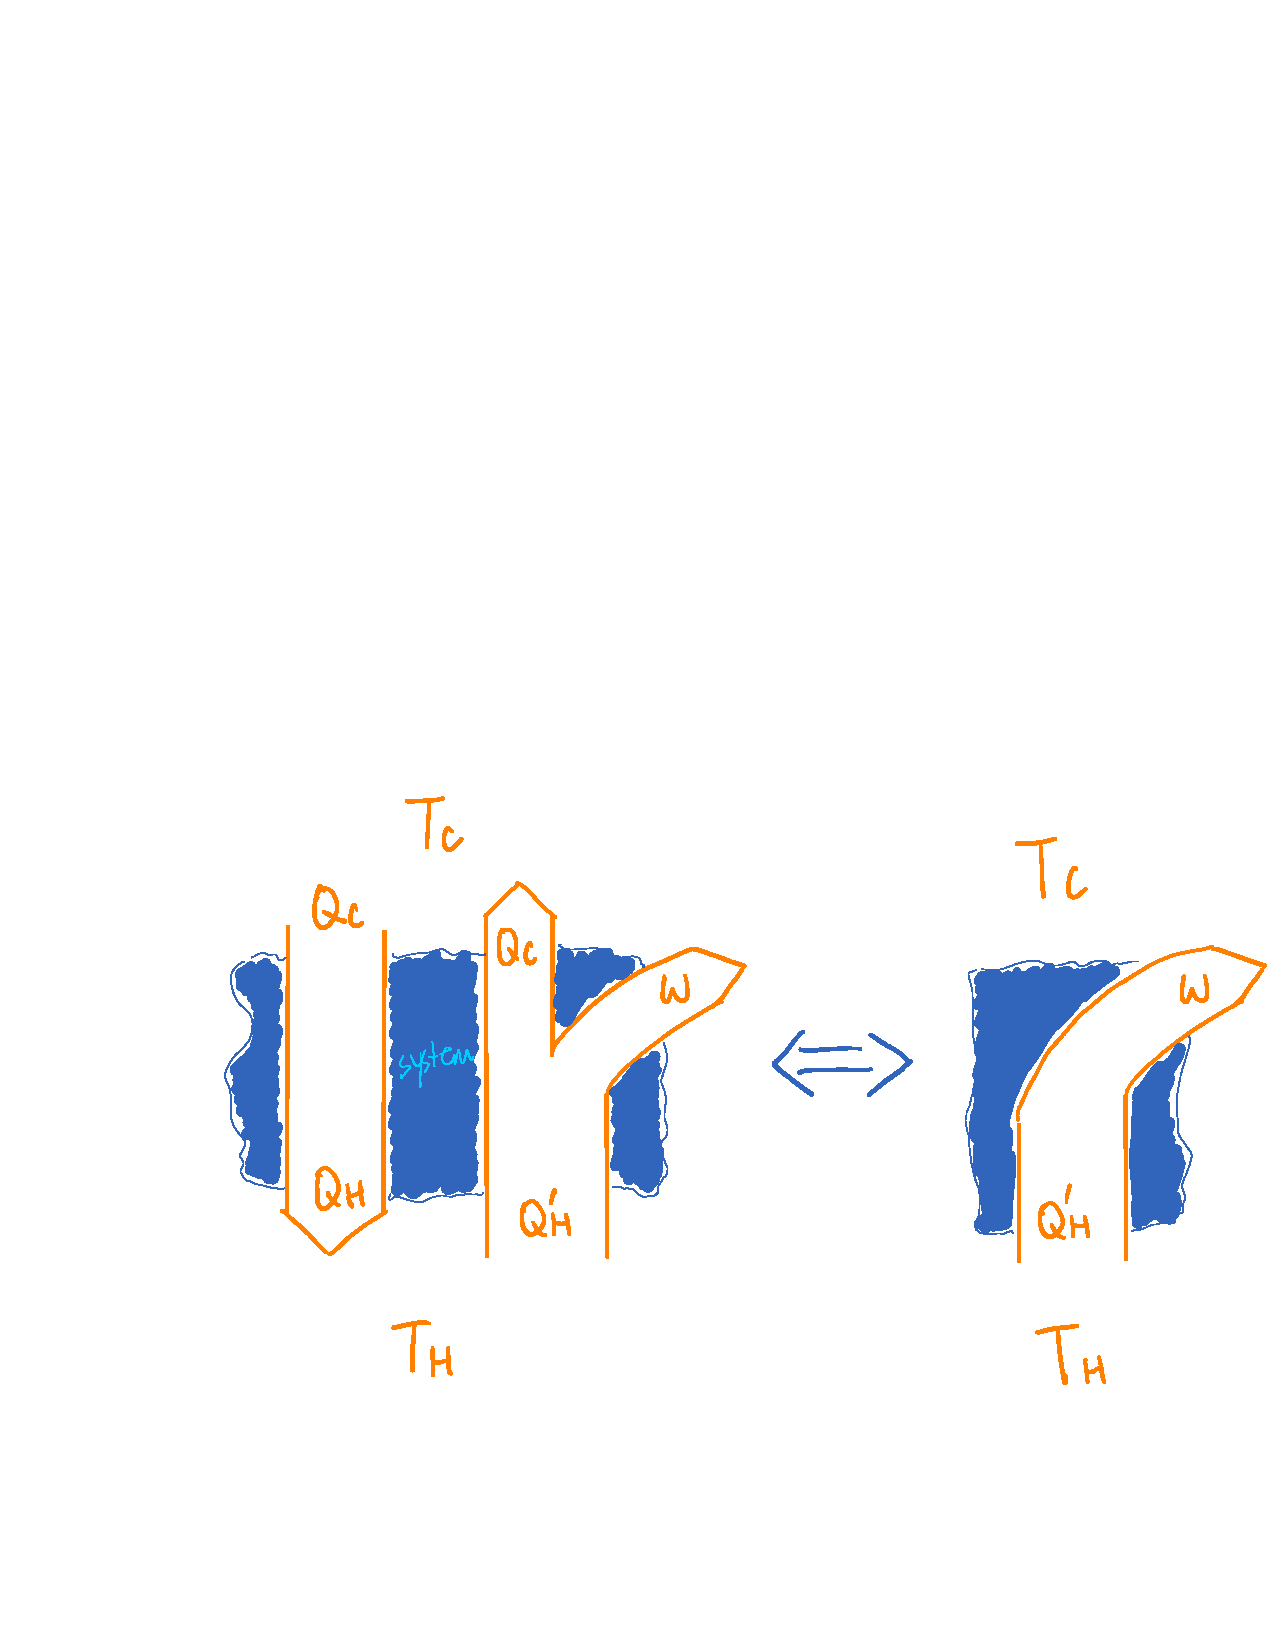
\includegraphics[scale=0.39]{2ndLaw1.pdf}
\end{center}


To show that $\mathcal{A}$ implies $\mathcal{B}$, we also proceed by contradiction, consider the following 100$\%$ efficient engine and an ordinary refrigerator, we can combine them and get a workless refrigerator and get a contradiction, so we conclude that $A$ implies $B$. 
\begin{center}
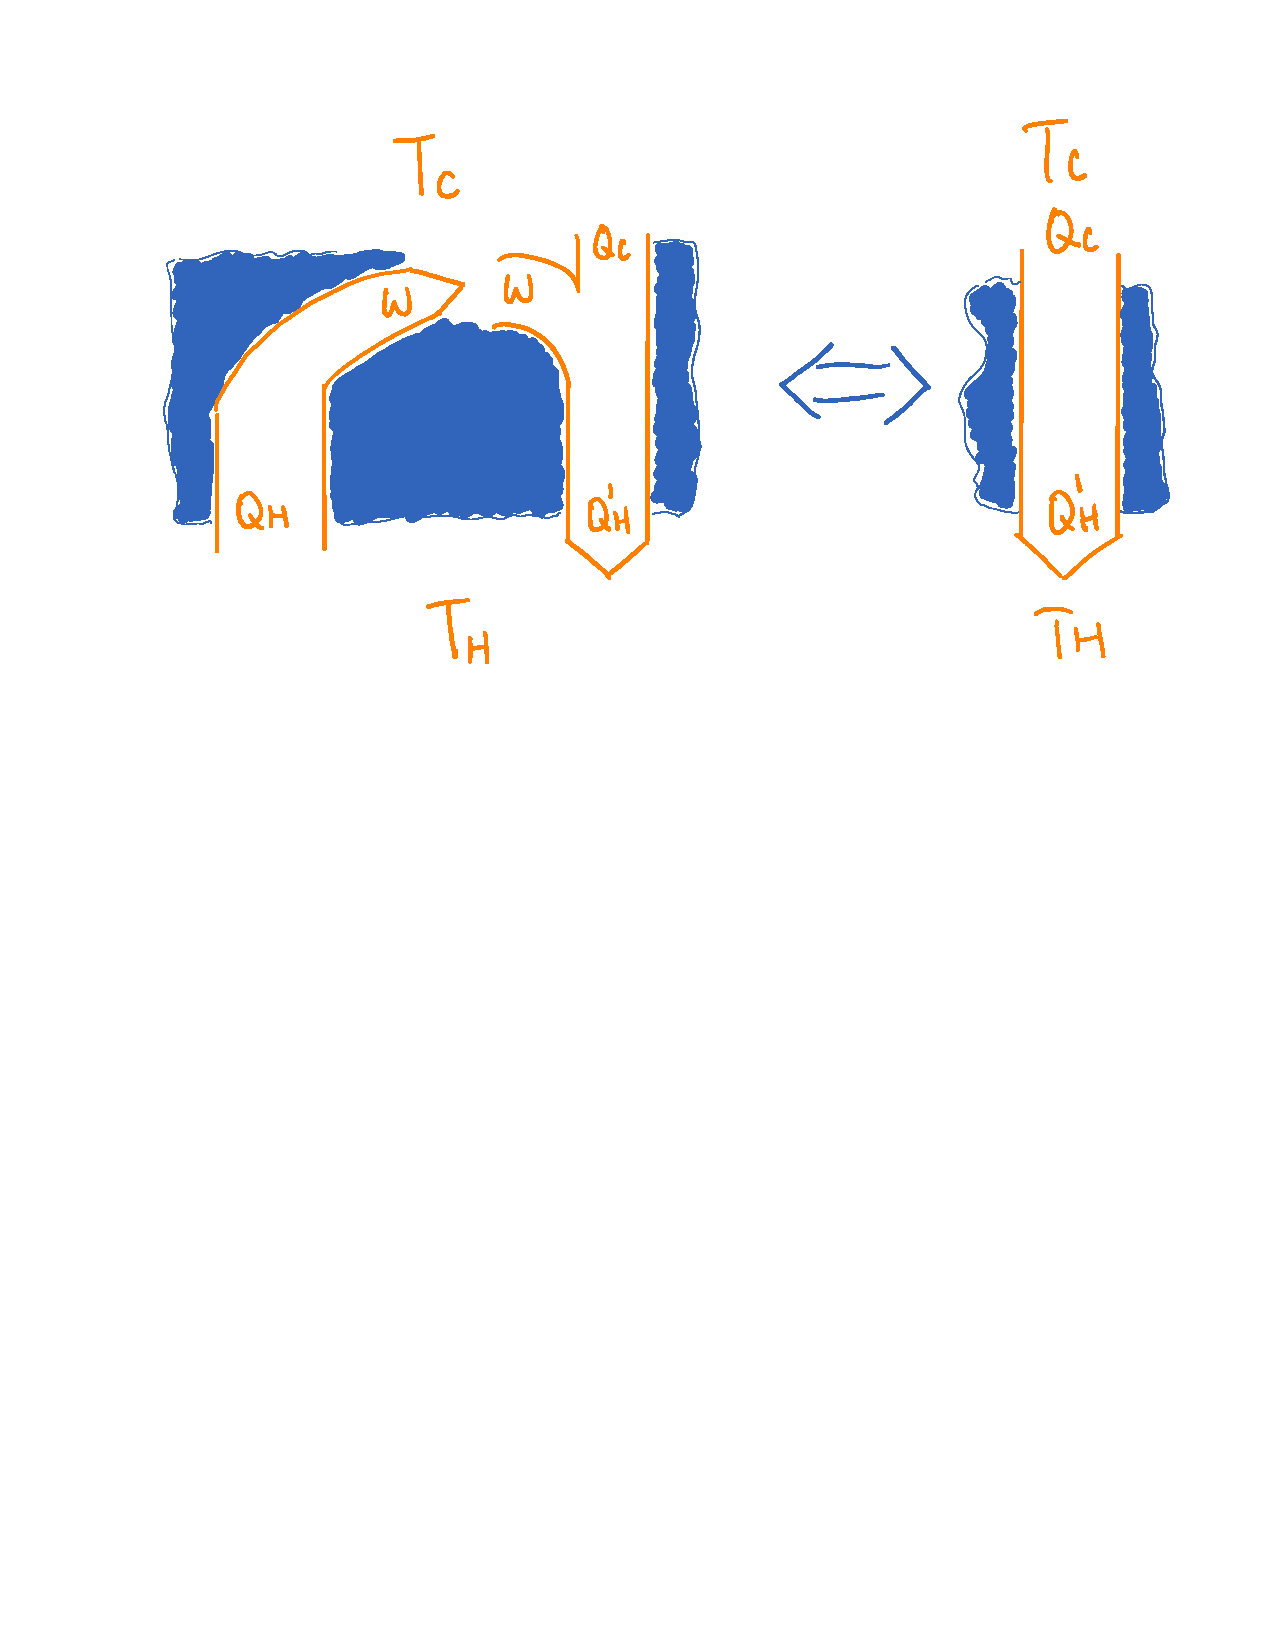
\includegraphics[scale=0.39]{2ndLaw2.pdf}
\end{center}





\newpage
\textbf{Entropy}\\

The Second Law of Thermodynamics express the "one way" aspect of thermodynamic process: "organized" becomes more "disorganized." This idea can be quantified, we consider the following example. Isothermal expansion of an ideal gas. Since the process is isothermal, we have $dT = 0$. For an ideal gas, the internal energy depends only on $T$, so we have $dU = 0$. Hence by the First Law of Thermodynamics, we have $0 = dQ - dW$, so $dQ = dW = pdV = \frac{nRT}{V}\,dV$, that is, we can write the following:
$$\frac{dQ}{T} = nR \frac{dV}{V}$$
When the gas expands, $\frac{dV}{V} > 0$, and hence $\frac{dQ}{T}>0$. Loosely, we can view $\frac{dQ}{T}$ as a measure of disorder in the system. 

\begin{defn}
The infinitesimal change in entropy, denoted as $dS$, in an infinitesimal reversible process at absolute temperature $T$ is given by $dS = \frac{dQ}{T}$. 
\end{defn}

Reversible process are those process that can be run in the reverse and give back the original result. For example, frictionless motion in mechanics, expansion or compression of a spring, isothermal expansion or compression of gas, ice melting in water at fixed temperature $0^\circ C$ are all reversible processes. \\

For the ice melting process at fixed temperature $0^\circ C$. When we add heat $\Delta Q$, $m = \frac{\Delta Q}{L_{ice}}$ of ice melts, and when we remove $\Delta Q$, $m = \frac{|\delta Q|}{L_{ice}}$ of ice forms. So at fixed temperature $T= 0^\circ C$, ice melting or forming is reversible. But ice melting in room temperature is not reversible, that involves heat spontaneously flowing from a hot body, the surroundings in the room, to a cold body, the ice itself, and that is a irreversible process.\\

Consider an isothermal process in which a total amount of heat $Q$ is added to the system. Then change in entropy of the system is given by the following:
$$\Delta S =S_f -S_i = \int_i^f dS = \int_i^f  \frac{dQ}{T} = \frac{Q}{T}$$
$Q$ has unit of $J$, and $T$ is the absolute temperature $K$, so entropy $S$ has units of $J/K$. \\


Consider the example, melting $1\, kg$ of ice at fixed temperature $T = 0^\circ C = 273\, K$, such process is reversible. Here we write $Q = m_{ice} \cdot L_{ice} =( 1\, kg)(334\ee^3\, J/kg) = 3.34\ee^5\,J$. Hence we can write:
$$\Delta S = \frac{Q}{T} = \frac{3.34\ee^5 \, J}{273\, K} = 1.22\ee^3 \, J/K$$
Melting ice increases the entropy as we see that $\Delta S >0$, hence ice crystal is more organized than liquid water.\\


The Second Law of Thermodynamics can also be stated as the "entropy version" as: \textit{The change in entropy of the entire system, denoted as $\Delta S_{all}$, is always greater than or equal to zero in all physical processes.} That is the entropy of an isolated system cannot decrease in a classical physical process.\\

The Second Law of Thermodynamics states that an isolated system develops toward the state of maximal entropy.\\ 

Note here, all those processes that we can draw on the pV-diagram are reversible. Hence we can use $\frac{dQ}{T}$ to describes the change of entropy of those processes. 

\textbf{The change in entropy is path independent.} In other words, entropy only depends on the state, not how it got to the state. The consequence of such is that for any cyclic process, the change in entropy is zero.\\
\newpage
Consider an ideal gas which expands from $V_a$ to $V_b$, with pressure change from $p_a$ to $p_b$, such process goes point point $a$ to point $b$. First we consider such process to be isothermal, at point $a$ and $b$, the gas has temperature $T_a = T_b = T$, then $\Delta S_{a \to b}$ simply given by $$\int_a^b \frac{dQ}{T } = \frac{Q_{a\to b}}{T} = \frac{W_{a\to b}}{T} = \frac{nRT\ln\left(\frac{V_b}{V_a}\right)}{T} = nR\ln\left(\frac{V_b}{V_a}\right)$$
Now consider such isothermal process is a a combination of a isobaric process from $a$ to $c$ with an isochoric process from $c$ to $b$. At $c$, say the gas has volume $V_c=V_b$ and pressure $p_c = p_a$. Then we can write the following:
$$\Delta S_{a \to b} = \Delta S_{a \to c} + \Delta S_{c \to b}$$
Here we have:
$$\Delta S_{a \to c} = \int_a^c \frac{dQ}{T} = \int_a^c \frac{nC_p\,dT}{T} = nC_p \ln\left(\frac{T_c}{T_a}\right) = nC_p\ln\left(\frac{T_c}{T} \right)$$
$$\Delta S_{c \to b} = \int_c^b \frac{dQ}{T} = \int_c^b \frac{nC_v\, dT}{T} = n C_v \ln\left(\frac{T_b}{T_c}\right) = nC_v \ln\left(\frac{T}{T_c}\right)$$
Combining we get:
\begin{align*}
\Delta S_{a\to b} &=  \Delta S_{a \to c} + \Delta S_{c \to b} \\ 
&= nC_p\ln\left(\frac{T_c}{T} \right) - nC_v \ln\left(\frac{T_c}{T}\right)\\
&= n(C_p-C_v)\ln\left(\frac{T_c}{T}\right)\\
&= nR\ln\left(\frac{p_cV_c/(nR)}{p_aV_a/(nR)} \right) \\
&= nR\ln\left( \frac{V_b}{V_a}\right)
\end{align*}
In such case, we see that the change in entropy is path independent. Now consider another path from $a$ to $c$. Say the gas first expands through adiabatic process from $a$ to $d$, then expands through isobaric process from $d$ to $b$. Then we can write:
$$\Delta S_{a \to b} = \Delta S_{a \to d} + \Delta S_{d \to b}$$
where we have:
$$\Delta S_{a \to d} = \int_a^d \frac{dQ}{T} = \int_a^d \frac{0}{T} = 0$$
$$\Delta S_{d \to b} = \int_b^d \frac{nC_p\, dT}{T} = nC_p \ln\left(\frac{T_b}{T_d}\right) = nC_p \ln\left(\frac{T}{T_d} \right)$$
We know that for an adiabatic process for an ideal gas, $TV^{\gamma-1}$ is a constant where $\gamma = \frac{C_p}{C_v}$. By the ideal gas law, we can write $$T= \left(\frac{nRT}{p}^{\gamma-1} \right) = \text{constant} \qquad \Rightarrow \qquad T^\gamma p^{1-\gamma} = \text{constant}$$
Hence in the context of our process, we can write the following:
$$T_a^\gamma p_a^{1-\gamma} = T_d^\gamma p_d^{1-\gamma}\qquad \Rightarrow \qquad T_d = T\left(\frac{p_a}{p_b}\right)^{\frac{1-\gamma}{\gamma}} \qquad\Rightarrow\qquad \frac{T}{T_d} = \left(\frac{p_b}{p_a}\right)^{\frac{1}{\gamma}-1}$$
Hence we can write:
\begin{align*}
\Delta S_{a \to b} &= \Delta S_{a \to d} + \Delta S_{d \to b} =  \Delta S_{d \to b} \\
&= nC_p \ln\left(\frac{T}{T_d}\right) 
= nC_p \ln\left( \left(\frac{p_b}{p_a}\right)^{\frac{1}{\gamma}-1}\right) 
= nC_p\left(\frac{1}{\gamma}-1\right) \ln\left( \frac{p_b}{p_a}\right) 
= nC_p\left(\frac{1}{\gamma}-1\right) \ln\left(\frac{nRT_b/V_b}{nRT_a/V_a} \right) \\
&= nC_p\left(\frac{1}{\gamma}-1\right)\ln\left(\frac{V_a}{V_b}\right)
=-nC_p\left(\frac{1}{\gamma}-1\right)\ln\left(\frac{V_b}{V_a}\right)
= -nC_p\left(\frac{C_v}{C_p}-1 \right)\ln\left(\frac{V_b}{V_a}\right)
= nR\ln\left(\frac{V_b}{V_a}\right)
\end{align*}
So we see that the change in entropy is also path independent in such process.\\

\newpage


More microstates implies more opportunity of being disorder. Entropy, in some sense, describes the number of microstates in a given macrostate. However, entropy $S$ has units of $J/K$, while the number of microstates is dimensionless. Notice that the Boltzmann's constant $k = 1.38\ee^{-25}\, J/K$ has exactly the same unit as entropy. \\

\begin{defn}[By Boltzmann]
Let $W_\C$ be the number of microstates in the macrostate $\C$. Then the entropy $S_{\C}$ of the macrostate $\C$ is given by $S_\C \coloneqq  k \ln(W_\C)$, where $k$ is the Boltzmann's constant. 
\end{defn}

By such definition of entropy, suppose the initial macrostate has number of microstates $W_i$, and the final macrostate has number of microstates $W_f$. Then the change in entropy from initial macrostate to final macrostate is given by the following:
$$\Delta S_{i\to f} = S_f - S_i = k\ln(W_i) - k \ln(W_i) = k \ln\left(\frac{W_f}{W_i}\right)$$
Here we see that, if $W_f > W_i$, then $\Delta S_{i\to f} >0$, and if $W_f< W_i$, then $\Delta S_{i \to f} <0$. The Second Law of Thermodynamics states that the change in total entropy of an isolated system must be greater than or equal to zero, this is a statement that suggests physics evolves toward the state of maximum entropy, or the sate of most microstates.\\


Example.\\
Calculate $\Delta S$ for 1 kg of ice melting at $0^\circ C$. 
$\Delta S = \int_{i}^f \frac{dQ}{T} = \frac{1}{T}Q = \frac{1}{T} m_{ice}L$
where $m_{ice}$ is the mass of the ice, and $L$ is the latent heat for ice becoming water. $\Delta S  = \frac{3.34\ee^{5}\, J}{273\, K} = 1.22\ee^3 \, J/K$
Here we see that $\Delta S > 0$, implies liquid water has more disorder than solid ice. \\

\newpage
\textbf{Carnot Cycle and Entropy}\\

In a Carnot Cycle, there are four points $a,b,c,d$. $a\to b$ is an isothermal expansion from $V_a$ to $V_b$. $b \to c$ is an adiabatic expansion from $V_b$ to $V_c$. $c \to d$ is an isothermal compression from $V_c$ to $V_d$, and $d \to a$ is an adiabatic compression from $V_d$ to $V_a$. Here we can write the following:
\begin{align*}
\Delta S_{Carnot} = \Delta S_{a \to b} + \Delta S_{b \to c} + \Delta S_{c \to d} + \Delta S_{d \to a} = \frac{Q_H}{T_H} + \frac{Q_C}{T_C} = 0
\end{align*}
This suggests that we have $\frac{Q_C}{Q_H} = - \frac{T_C}{T_H}$. 
The efficiency of a Carnot engine is given by: 
$$e_{Carnot} = 1 + \frac{Q_C}{Q_H} = 1- \frac{T_C}{T_H}$$
One the other hand, one might write the followings:
$$Q_H = W_{a \to b} = nRT_H \ln\left(\frac{V_b}{V_a} \right) \qquad Q_C = W_{c \to d} = nRT_C \ln\left(\frac{V_d}{V_c}\right) \qquad \frac{V_c}{V_d} = \frac{V_b}{V_a}$$
Combining we also get $\frac{Q_c}{Q_H} = -\frac{T_C}{T_H}$.\\


\textbf{Carnot engine is the most efficient engine.}\\

Consider a cycle of points $a,b,c,d$. $a \to b$ is isothermal expansion, $b\to c$ is isochoric, $c \to d$ is isothermal compression, and $d \to a$ is isochoric. Say the volume of the gas at $d$ and $a$ is $V$, and the volume of the gas at $c$ and $b$ is $rV$ for some scalar $r$. Here the efficiency of this cycle is given by $e = 1+ \frac{Q_C}{Q_H}$. In such cycle, we can write the followings:
$$Q_{a \to b} = W_{a \to b} = nRT_H \ln\left( \frac{V_b}{V_a}\right) = nRT_H\ln(r) > 0$$
$$Q_{c \to d} = W_{c \to d} = nRT_C \ln\left( \frac{V}{rV}\right) = -nRT_C \ln(r) < 0$$
Here we see that $Q_{a \to b}$ contributes to $Q_H$  because it is greater than zero, and $Q_{c \to d}$ contributes to $Q_C$ because it is less than zero. Moreover, we can write:
$$Q_{b \to c} = nC_v(T_C-T_H) = -nC_V(T_H-T_C) < 0$$
$$Q_{d \to a} = nC_V(T_H-T_C) >0$$
Hence we see that $Q_{b \to c}$ contributes to $Q_C$ and $Q_{d\to a}$ contributes to $Q_H$. Now we can write the followings:
$$Q_H = Q_{a \to b} + Q_{d \to a} = nRT_H\ln(r) + nC_v(T_H - T_C)$$
$$Q_C = Q_{b \to c} + Q_{c \to d} = -nC_v(T_H-T_C)-nRT_C\ln(r)$$
Combining we get the following:
\begin{align*}
e = 1+ \frac{Q_C}{Q_H} &= 1- \frac{nRT_C\ln(r) + nC_v(T_H-T_C)}{nRT_H\ln(r)+nC_v(T_H-T_C)} = 1-\frac{\frac{T_C}{T_H}\ln(r) + \frac{C_v}{R}\left(1-\frac{T_C}{T_H}\right)}{\ln(r) + \frac{C_v}{R}\left( 1- \frac{T_C}{T_H}\right)}
\end{align*}
where $r >1$. When we have $r \to \infty$, $e \to 1-\frac{T_C}{T_H} = e_{Carnot}$. So this cycle approaches the Carrnot Cycle when $r$ tends to infinity. On the other hand, when $r \to 1$, then $e \to 0$. \\

At finite values of $1< r < \infty$, suppose we have $\frac{T_C}{T_H} = \frac{1}{2}$, and $\frac{C_v}{R} = \frac{3}{2}$, then we have: 
$$e = 1-\frac{\frac{1}{2}\ln(r)+\frac{3}{2}\left(1-\frac{1}{2}\right)}{\ln(r)+\frac{3}{2}\left(1-\frac{1}{2}\right)} < e_{Carnot}$$

This is an example of an engine cycle with efficiency $e < e_{Carnot}$. But in general, we have $e_{Carnot} \geq e$ for $e$ being the efficiency of arbitrary engine. \\

If there exists and engine with an efficiency $e > e_{Carnot}$, then one can write:
$$1+ \frac{Q_C}{Q_H} > 1- \frac{T_C}{T_H}\qquad \Rightarrow \qquad \frac{Q_C}{T_C}+\frac{Q_H}{T_H} >0$$
and one can show that this is in conflict with the Second Law of Thermodynamics. 
\newpage

Clausius' Inequality states the following:
$\Delta S \geq \int \frac{dQ}{T}$
for non-reversible processes, and equality holds for reversible processes.\\

Thermodynamics is everywhere in our daily lives. Including morning coffee and tea, heating and cooling system. Transposition such as cars and trucks; Power plants that uses fossil fuel, nuclear fuel; Heat transfer system such as double or triple pane windows, or insulating house; All these involves thermodynamics. \\

In modern fundamental physics research, thermodynamics play a role as the following examples:
\begin{enumerate}
\item CMB - Cosmic Microwave Background.\\ Very uniform temperature distribution across all directions we look into space, but the tiny derivatives $\delta T$ and their correlations across the sky tell us about the structure formation in the Early Universe and the composition of the universe, around $5\%$ of ordinary matters, around $27\%$ dark matters, and around $68\%$ dark energy. Current research also seeks to improve the detailed measurements of the CMB and understand the equation of state in the early universe. One can search about the Atacama Cosmological Telescope, and the DESI (Dark Energy Spectroscopy Experiment) for details about this topic.
\item Critical Phase Transitions\\
Scale invariant theories in four dimensions, three space dimensions and one time dimension, are conjectured to have enhanced symmetry called the conformed symmetry. Such theories, the Conformal Field Theories, are a special class the theories in the framework of Quantum Field Theories. Modern research seeks to understand the incredibal rich and vast landscape of all Quantum Field Theories, which include the standard model of partical physics, and in particular there has been amazing progress in understanding the Conformal Field Theories, this includes the 3d Ising Model which describes the physics of water at the critical point and ferromagnets at the Curie temperature. Thus, fundamental research in Quantum Field Theories is relevant for defining the properties of continuous phase transitions, a similar application is the model for a critical phase transition in Helium-4. 
\item Black Holes\\
In classical mechanics, we have learned about the escape velocity $$V = \sqrt{\frac{2GM}{R}}$$
Combining with the Maxwell-Boltzmann distribution for molecules' velocities, we could understand why Earth does not have $He$ or $H_2$ in atmosphere. While if we keep $M$ fixed and decrease $R$, the escape velocity increases. From Special Relativity, we must have $v<c$. So when $v_e > c$, light will not even be able to escape, and in such case we call the object a black hole. A black hole is a region in spacetime from which not even light can escape.
$$c = V = \sqrt{\frac{2GM}{R_s}} \qquad\Rightarrow \qquad R_s = \frac{2GM}{c^2}$$
Here $R_s$ is called the Schwarzschild Radius. Given $M$, nothing can escape from inside $R_s$. For $M $ being the mass of the Earth, $R_s^{Earth} \approx 8.8\, mm$. Black holes are relevant in Astrophysics, there is a super massive black hole at the center of our Galaxy, with $M_{BH} \approx \ee^6 $ solar masses. The Event Horizon Telescope reported the first picture of a Black Hole, at the center of the M87 Galaxy, in April 2019. It is actually a picture of matter swirling around the Black Hole. First observation of gravitational waves from inspiral and merger of two enormously massive black holes, one with $36$ solar masses and one with $29$ solar masses, as well as other observations, was done by LiGO Collaboration announed first results in February 2016. Classically, nothing escape from a Black Hole, but in 1974-1975, Stephen Hawking published a calculation that showed that Black Holes radiate thermally just like a blackbody. So there is theritically radiation from a black hole just like the Planck Spectrum with temperature $T = \frac{\hbar c^2}{8\pi GkM}$. Large massive black holes have very low temperature, and we have not observed Hawking radiation. Smaller blakc holes are hotter and evaporate faster, as the black hole evaporates, it losses energy, and since $E = mc^2$, it means that the black hole's mass decreases. One can show $dM = T dS$, where $dS = \frac{kdA}{4l_p^2}$, where $A$ is the are of the black hole horizon $A = 4\pi R_s^2$, $l_p$ is the Planck length $l_p^2 = \frac{G\hbar}{c^3}$, and $\hbar = \frac{h}{2\pi}$ with $h$ being the Planck's Constant. Here we must have $dA \geq 0$, and with $dS \geq 0$, which comes from the Second Law of Thermodynamics. Compare $dM = T dS$, $dS \geq 0$, with $dQ=T dS$, $dS\geq 0$, black holes are thermodynamic systems, write $S_{BH} = \frac{kA}{4l_p^2}$. Here entropy of a black hole scales with the are of the event horizon. Entropy counts microstates, $S = k\ln(w_i)$, so the number of microstate for a $1$ molar mass black hole is given by $w = e^{S_{BH}/k} \approx e^{10^{77}}$.  The number of microstates responsible for the entropy of a $1$ molar mass black hole is much larger than the number of Hydrogen atoms in the Sun. String Theory can account for this black hole entropy. 
\end{enumerate}



\newpage















\section{\color{red} Wave}
There are two types of mechanical waves, the transverse wave and the longitudinal wave. The motion of a transverse wave is perpendicular to the wave traveling direction. The motion of a longitudinal wave is parallel to the wave traveling direction. In common, there is no net movement of the particles or matter. There is something that moves to transport energy and information in the waves, but the matter itself is not transported.\\

\textbf{Transverse Wave}\\
Suppose there is a bob going up and down between points $A$ and $-A$ on the $y$-axis. A rope lying parallel to the $x$-axis is connected to the bob. Each point on the rope moves up and down in the $y$-direction as time $t$ passes by, but the rope itself has no motion in the $x$-direction. Here $A$ is called the amplitude of the wave, which is the maximal transverse displacement. Wavelength is defined to be the distance between wave tops, denoted by $\lambda$, with units of meters. Period is defined to be the time it takes for the wave to advance one full wave length, denoted as $T$ with unit seconds. Frequency is defined to be $f= \frac{1}{T}$, with unit $\frac{1}{s}\coloneqq Hz$. The angular frequency of the wave, denoted as $\omega$, is defined by $2\pi f$, with unit $\frac{rad}{s}$. Speed of the wave propagation is given by $v = \frac{\lambda}{T} = \lambda f$, with unit $m/s$.\\
\begin{center}
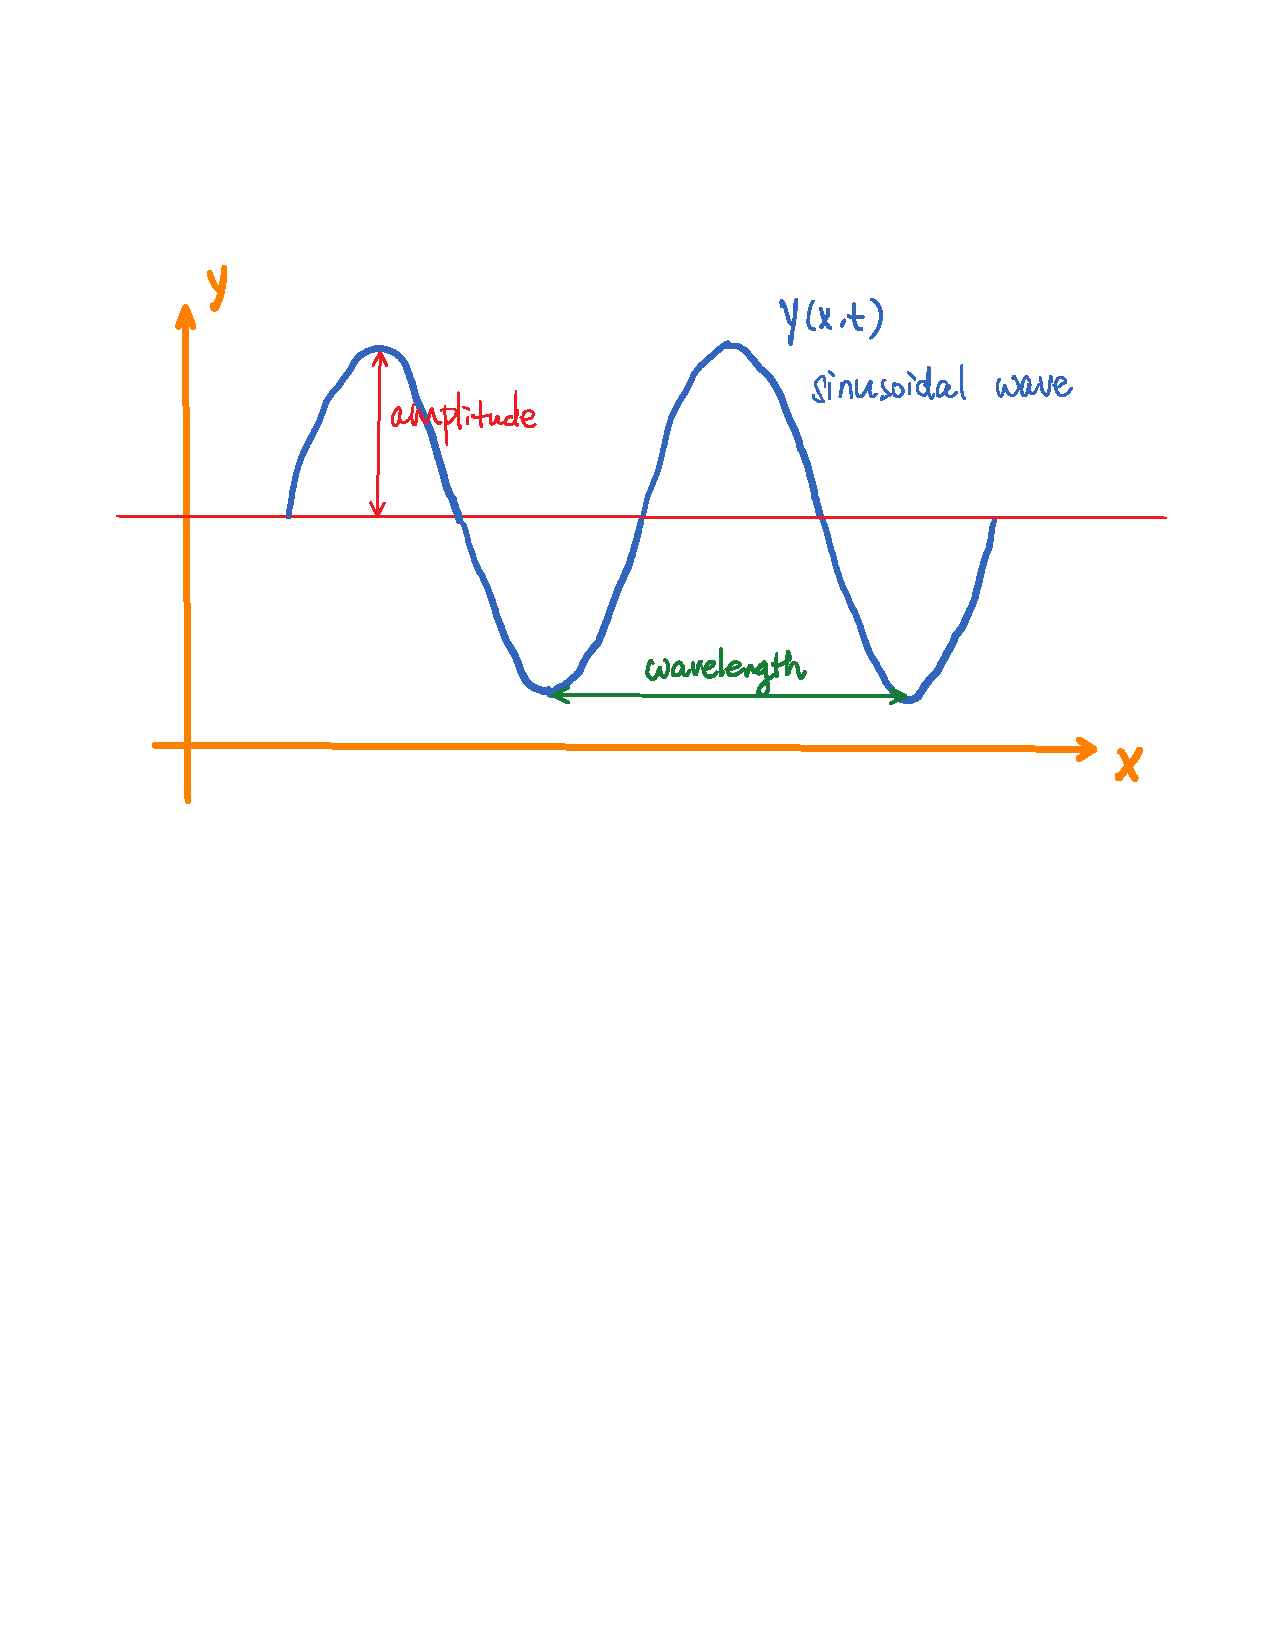
\includegraphics[scale=0.75]{wave.pdf}
\end{center}
\textbf{Sinusoidal Waves}\\
For a sinusoidal wave, the position $y(x,t)$ of the wave can be described by the following: 
$$y(x,t) = A\cos(kx \pm \omega t)$$
Here $y(x,t) = A\cos(kx +\omega t)$ indicates that the wave is moving in the negative $x$-direction. $y(x,t) = A\cos(kx - \omega t)$ represents that the wave is moving in the positive $x$-direction. $k = \frac{2\pi}{\lambda}$ is called the wave number, with unit $\frac{rad}{m}$. Note here for $x = 0$, we have $y(0,t) = A\cos(\pm \omega t) = A\cos(\omega t)$. Note here, the function $y(x,t)$ describes the motion of the wave (the rope, or string, or anything that carries the information and the energy of the wave) at given position $x$ and at given time $t$. Here we can also rewrite $y(x,t)$ as the followings:
$$y(x,t) = A\cos\left( k \left(x \pm \frac{\omega }{k}t\right) \right)$$
$y(x,t)$ represents the motion of one of the wave tops when $x \pm \frac{\omega }{k} t = 0$ is satisfied, this describes the motion of one of the wave tops, and here rearranging, we use the following to describe the motion of the wave top:
$$x= \mp \frac{\omega}{k}t$$
with $\frac{\omega}{k}$ being the speed of the propagation of the wave:
$$v = \lambda f = \frac{\lambda}{2\pi}2\pi f = \frac{\lambda}{2\pi}\omega = \frac{\omega }{k} \qquad \Rightarrow\qquad  k = \frac{2\pi }{\lambda}$$
For given $x$, the speed of a point in the $y$-direction is given by the following:
$$\dot{y}\coloneqq \frac{\partial y}{\partial t} = \omega A \sin(kx - \omega t)$$
The acceleration of the wave is given by:
$$\ddot{y} = \frac{\partial^2 y}{\partial t^2} = -\omega^2 A \cos(kx-\omega t) = -\omega^2 y(x,t)$$
Here we conclude the following:
$$\frac{\partial^2 y}{\partial t^2} = -\omega^2 y$$
Note here we also get:
$$\frac{\partial^2 y}{\partial x^2} = -k^2 A \cos(kx-\omega t) = -k^2y(x,t)$$
Note here $v = \frac{\omega }{k}$, combining we obtain the wave equation:
$$\frac{\partial^2 y}{\partial x^2} = -\frac{1}{v^2}\omega^2 y = \frac{1}{v^2} \frac{\partial^2 y}{\partial t^2}$$
Here we see that the sinusoidal waves are solutions for any $k$ and $\omega$ with $v = \frac{\omega}{k}$ to the wave equation.

\newpage
\textbf{Energy in Wave}\\
Consider s string of uniform mas density $\mu$, that is, we can write $dm = \mu dl$ with infinitesimal length $dl$. Power in one wavelength of the wave carried by the string is given by:
$$P_{av} = \frac{1}{2}\mu\omega^2 A^2 v$$
where $\mu$ is the mass density, $\omega$ is the angular frequency, $A$ is the amplitude of the wave, and $v$ is the speed of the wave. Here we note that the energy carried by the string is proportional to the square of the amplitude of the wave. If a string has tension $T_{string}$, then we can write:
$$v = \sqrt{\frac{T_{string}}{\mu}}$$
Hence we can write the following:
$$P_{av} = \frac{1}{2}\sqrt{\mu T_{string}}\ \omega^2 A^2 $$


\hfill\break\hfill\break

\textbf{Wave Equation}\\
Wave equation is a second order partial differential equation:
\begin{align*}
\frac{\partial y}{\partial x^2} - \frac{1}{v^2}\frac{\partial^2 y}{\partial t^2} = 0
\tag{1}
\end{align*}
describes a wave traveling in the $y$-direction. Here we see that equation (1) is a linear homogeneous equation. \\

\textbf{Superposition Principle} states that, if $y_1(x,t)$ and $y_2(x,t)$ are solutions to the wave equation (1) with specified speed $v$, then any linear combination of $y_1$ and $y_2$ also solve such wave equation (1) with speed $v$. That is, $y_3(x,t) = a\cdot y_1(x,t) + b\cdot y_2(x,t)$ solves wave equation (1) with speed $v$, where $a,b \in \R$ are arbitrary. The Superposition Principle is useful in many topics in Physics, such was mechanical/EM waves, interference/diffraction in optics, Fourier analysis, Quantum Mechanics, and so on. \\

Example.\\
Suppose we have two solutions to the equation (1) with specified $v$. $y_1(x,t) = A\cos(kx-\omega t)$ and $y_2(x,t) = A\cos(kx+\omega t)$. Then by the Superposition Principle, we can write the following:
$$y_3(x,t) = y_1(x,t) - y_2(x,t) = A(\cos(kx-\omega t)-\cos(kx+\omega t)) = A\sin(kx)\sin(\omega t)$$
here $y_3(x,t)$ is also a solution to equation (1) with the specified $v$. Such wave is called the Standing Wave.

\newpage
\textbf{Electromagnetic Waves}\\
Maxwell's Equations in Vacuum:
\begin{align*}
\vec{\nabla}\cdot \vec{E} = 0 \qquad \qquad \vec{\nabla}\cdot \vec{B} = 0 \qquad\qquad \vec{\nabla}\times\vec{E} = -\frac{\partial \vec{B}}{\partial t} \qquad \qquad \vec{\nabla}\times \vec{B} = \mu_0 \epsilon_0 \frac{\partial \vec{E}}{\partial t}
\end{align*}
where $\epsilon_0$ is the vacuum permittivity, and $\mu_0$ is the vacuum permeability. Here we can write:
$$\vec{E} = \vec{E}(x,y,z,t) = \begin{bmatrix}E_x(x,y,z,t) \\ E_y(x,y,z,t) \\ E_z(x,y,z,t)\end{bmatrix} \qquad \qquad\qquad \vec{B} = \vec{B}(x,y,z,t) = \begin{bmatrix}B_x(x,y,z,t) \\ B_y(x,y,z,t) \\ B_z(x,y,z,t)\end{bmatrix}$$
Maxwell's Equations are a set of coupled first order partial differential equations. Now we simplify the setup by assuming that $\vec{E} = (0,E,0)$ and $\vec{B} = (0,0,B)$, where $E$ and $B$ are functions of $(x,y,z,t)$. Note that we have $\vec{E}$ being orthogonal to $\vec{B}$. Now we examine Maxwell's Equations with this assumptions:
\begin{align*}
\vec{\nabla}\cdot \vec{E}= \frac{\partial E}{\partial y}= 0 \qquad \Rightarrow \qquad E \text{ is independent of }y
\end{align*}
\begin{align*}
\vec{\nabla}\cdot \vec{B} = \frac{\partial B}{\partial z} = 0 \qquad \Rightarrow \qquad B \text{ is independent of }z
\end{align*}
\begin{align*}
\vec{\nabla}\times \vec{E} = -\frac{\partial \vec{B}}{\partial t} \qquad\Rightarrow \qquad -\frac{\partial E}{\partial z} = 0,\ \  -\frac{\partial E}{\partial x} = \frac{\partial B }{\partial t}\qquad \Rightarrow \qquad E \text{ is independnet of }z
\end{align*}
\begin{align*}
\vec{\nabla}\times \vec{B} = \mu_0 \epsilon_0 \frac{\partial \vec{E}}{\partial t} \qquad \Rightarrow \qquad \frac{\partial B}{\partial y} = 0, \ \ \frac{\partial B}{\partial x} = -\mu_0 \epsilon_0 \frac{\partial E}{\partial t}\qquad \Rightarrow \qquad B \text{ is independent of }y
\end{align*}
Here we conclude that $E(x,t)$ is independent of $y,z$, and $B(x,t)$ is independent of $y,z$. We want to look for a second order differential equation to describe the electromagnetic waves:
\begin{align*}
\frac{\partial E}{\partial x} = -\frac{\partial B}{\partial t} \qquad \qquad \qquad -\frac{\partial B}{\partial x} = \mu_0 \epsilon_0 \frac{\partial E}{\partial t}
\end{align*}
Here we get:
$$\frac{\partial^2 E}{\partial x^2} = -\frac{\partial^2 B}{\partial x \partial t} \qquad \qquad \qquad -\frac{\partial^2B}{\partial t \partial x} = \mu_0\epsilon_0 \frac{\partial^2 E}{\partial t^2}$$
Combining the two equations we get the following:
$$\frac{\partial^2 E}{\partial x^2} = \mu_0 \epsilon_0 \frac{\partial^2 E}{\partial t^2}$$
Here we obtain a wave equation with speed $v = \sqrt{\frac{1}{\mu_0 \epsilon_0}} = c \approx 3.0\ee^8\,m/s$.
Similarly, we will find:
$$\frac{\partial^2 B}{\partial x}- \frac{1}{c^2} \frac{\partial^2 B}{\partial t^2} = 0$$
The Maxwell's Equations in vacuum imply the wave equations with speed $c$ for the components of the electromagnetic fields $E$ and $B$ that are not independent but must obey $\vec{E}$ perpendicular to $\vec{B}$. Here we made a particular ansatz for $\vec{E}$ and $\vec{B}$. More generally, it is also true that Maxwell's Equations in vacuum implies the wave equations described above, and the direction of propagation is $\vec{E}\times \vec{B}$. \\

Energy flux in electromagnetic wave is given by the Poynting vector:
$$\vec{S} = \frac{1}{\mu_0}\vec{E} \times \vec{B}$$


Example.\\
Consider a sinusoidal electromagnetic wave described by $E = E_{max}\cos(kx-\omega t)$, with $c = \frac{\omega}{k}=\lambda f$. Since we have $\frac{\partial E}{\partial x}=  -\frac{\partial B}{\partial t}$, so we know that $\frac{\partial B}{\partial t} = - \frac{\partial E}{\partial x} = kE_{max} \sin(kx-\omega t)$, which implies:
$$B = \frac{k}{\omega}E_{max} \cos(kx-\omega t)=\frac{1}{c}E_{max}\cos(kx-\omega t)$$
Here we see that the electric field and the magnetic field oscillate in phase as the wave propagates. Moreover, we have the following:
$$|\vec{S}| = \frac{1}{\mu_0}|\vec{E} \times \vec{B}| = \frac{1}{\mu_0}|\vec{E}| \cdot |\vec{B}| = \frac{1}{\mu_0 c} E_{max}^2 \cos^2(kx-\omega t)$$
Hence integrating over a wavelength of the wave, we get:
$$S_{average} = \frac{1}{2}\frac{1}{\mu_0 c} E_{max}^2 = \frac{1}{2}\epsilon_0 c E_{max}^2$$
The momentum is electromagnetic wave is given by $$P_{rad} = \frac{S_{average}}{c} \qquad \qquad \text{if the wave is totally absroved}$$
$$P_{rad} = 2\frac{S_{average}}{c} \qquad \qquad \text{if the wave is totally reflected}$$
Electromagnetic radiation can also be standing waves. As in microwaves, with a particular wavelength $\lambda = 12.2\, cm$, which can be strongly absorbed in water. Here energy is absorbed by the molecules, and hence the kinetic energy of the molecules increases, and so the temperature increases. 


\newpage
\textbf{Light}\\

In 1600's, Newton and Galileo believed that light was a particle. Around 1665, wavelike properties of light were discovered, such as the light diffraction, and wave theory of light was formulated by Huygens. Around 1801, Young's Double-Slit Experiment exhibits wavelike nature of light. Around 1873, Maxwell predicted EM waves. By early 1905, evidences of light as a particle were discovered, such as the photoelectric effect, and the Compton scattering. Light is a particle called the photon, which is massless, traveling at the speed of light, with energy $E= hf$, momentum $p = \frac{E}{c}$, and $c = \lambda f$. In fact, light is both particles and waves. Moreover, all particles have a wavelike behavior, such phenomenon is called the Particle-Wave Duality.\\













\newpage
\textbf{Optics}\\

Optics is a topic about light going through some materials. Up to now, we have discussed about electromagnetic waves traveling in vacuum, formulated by Maxwell's Equations in vacuum, in such a way that $\vec{E}$ is orthogonal to $\vec{B}$, and wave traveling in the direction of $\vec{E}\times \vec{B}$ at the speed of light $c = \frac{1}{\sqrt{\mu_0\epsilon_0}}$. In other materials, we need to replace $\epsilon_0$ with the permittivity of the material $\epsilon$, and $\mu_0$ with the permeability of the material $\mu$, hence the speed of the electromagnetic wave is given by the following:
$$v = \frac{1}{\sqrt{\mu \epsilon}}$$ 

The Index of Refraction of a material is defined by the following:
$$n = \frac{c}{v}$$
Note here the index of refraction of vacuum is always $1$. The index of refraction of air is around $n=1.0003$ at room temperature. For glasses, the index of refraction ranges from $1.5$ to $2$. For diamonds, the index of refraction is around $2.417$. Index of refraction is always greater than or equal to $1$ for all materials, which means that light tends to slow down inside materials other than vacuum.\\

\begin{center}
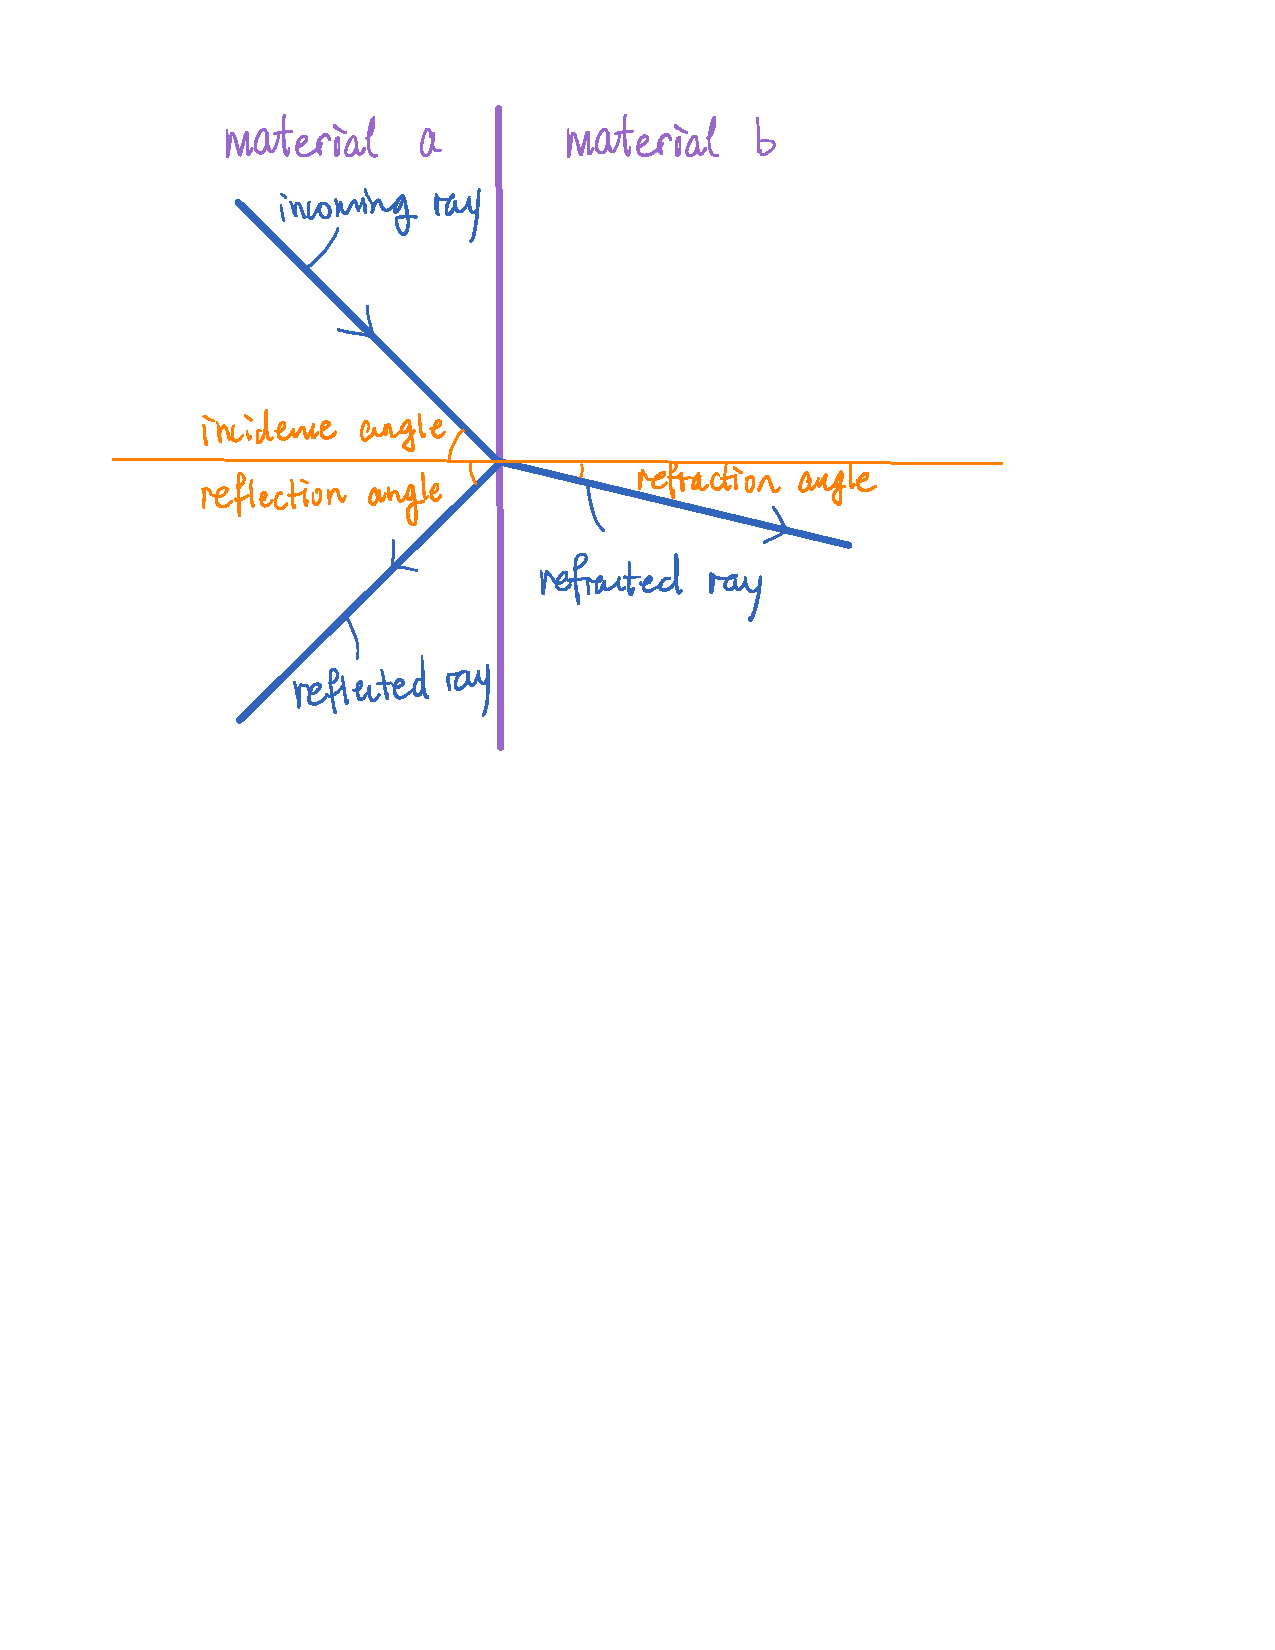
\includegraphics[scale=0.8]{incidencePlane.pdf}\\
\end{center}

\textbf{Laws of Reflection and Refraction} state the followings:
\begin{enumerate}[topsep=3pt,itemsep=-1ex,partopsep=1ex,parsep=1ex]
\item The incident ray, the reflected ray, and the refracted ray all lie in the same plane, called the plane of incidence.  
\item The degree of incident angle is equal to the degree of reflection angle.
\item Let $\theta_a$ denote the incidence angle, and let $\theta_b$ denote the refraction angle, let $n_a$ denote the index of refraction of the material in which the incoming ray is traveling through, and let $n_b$ denote the index of refraction of the material in which the refraction ray is traveling through. Here we have the Snell's Law holds:
$$n_a\sin(\theta_a) = n_b \sin(\theta_b)$$  
\end{enumerate}

Note here, the laws of reflection and refraction only apply to perfectly smooth surfaces. From a rough surface, we get diffuse reflection. \\
\newpage
In the following we will derive the laws of reflection and refraction. There are two ways to do so, one might use Huygens' principle, which follows the wave fronts, or, one might use Fermat's principle of least time of all paths between two points, light travels along the path which has extreme time. In the following we will use Huygens' principle:

\begin{center}
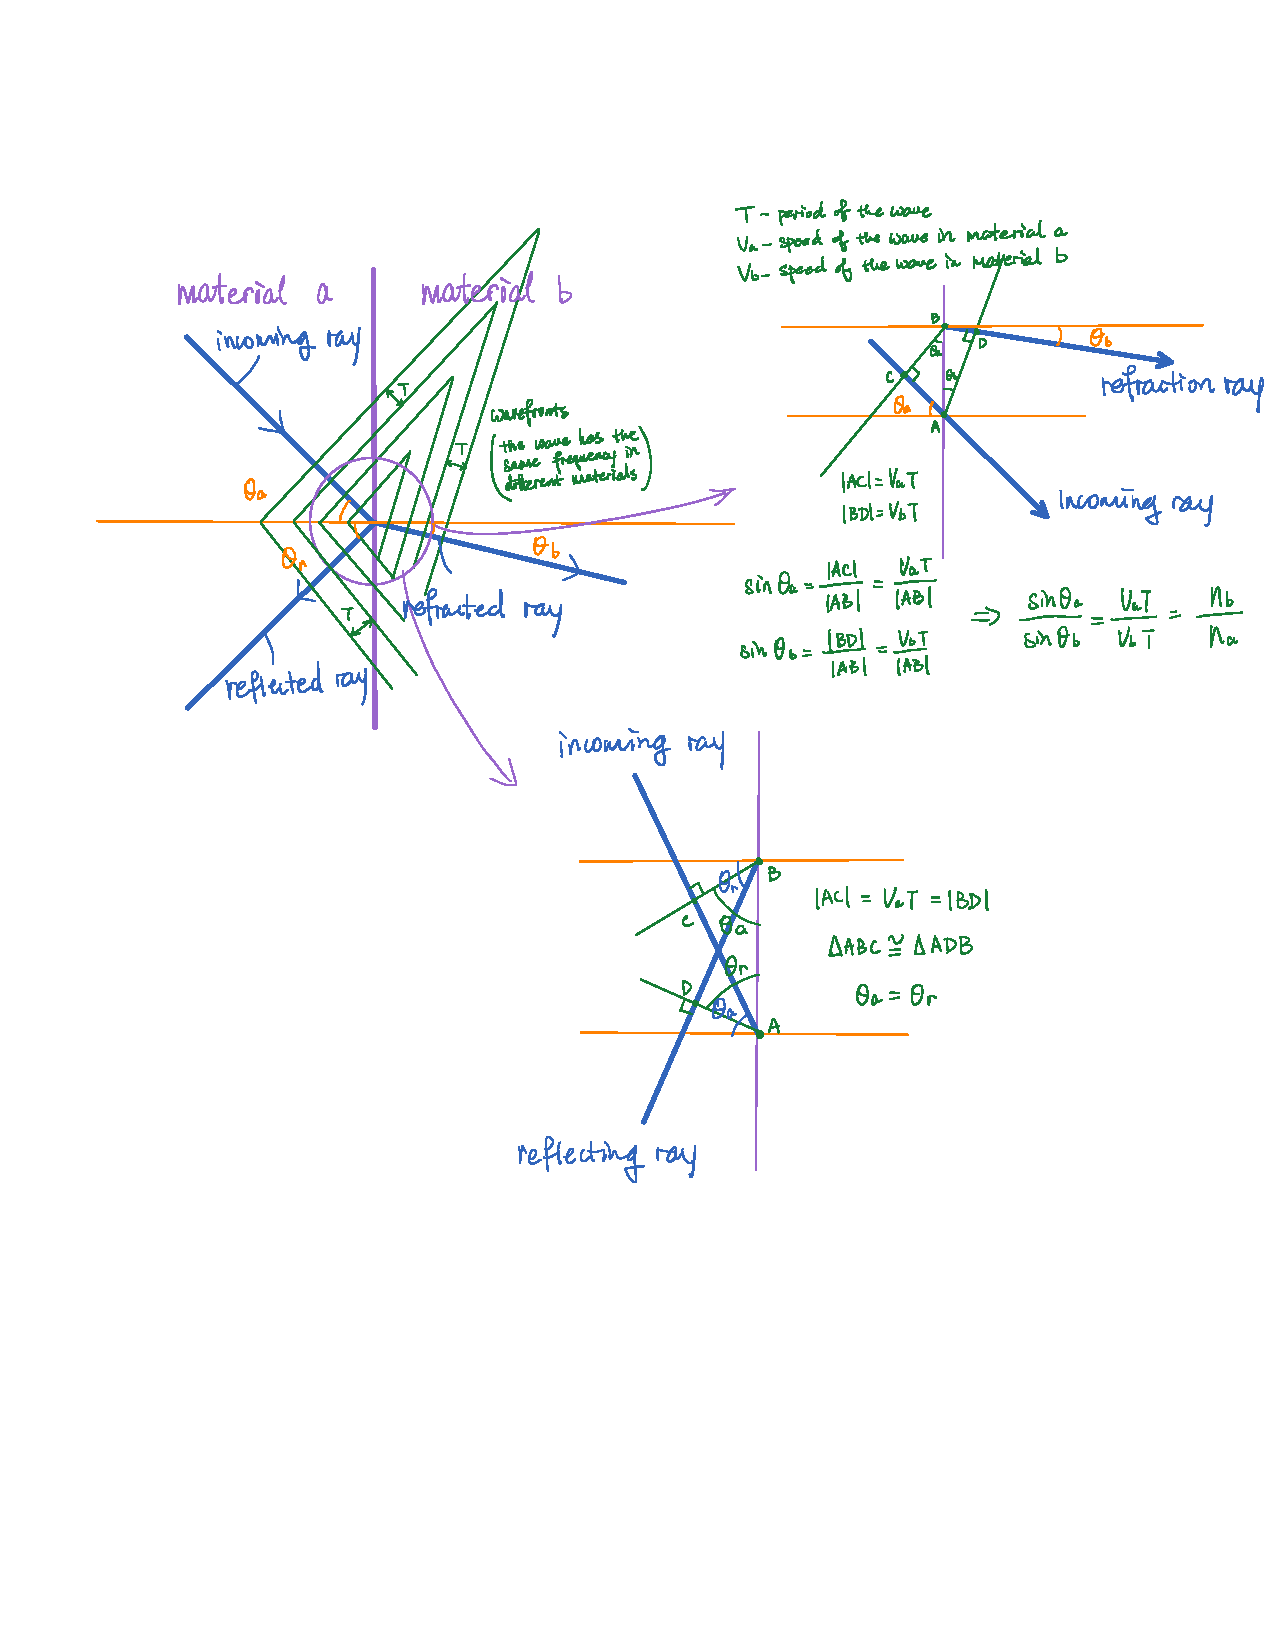
\includegraphics[scale=0.8]{derivRefrRefl.pdf}
\end{center}
\newpage
Lights are electromagnetic waves, which are the oscillating electric and magnetic fields. Material response depends on frequency of the oscillation of the electric and magnetic fields, so the index of refraction of a material depends on $\lambda$ of the wave. Typically, $n$ is smaller for light of larger wavelengths, and larger for light of shorter wavelengths, so red light would typically has smaller index of refraction than the blue light does. Snell's Law applies to each wave length, that is, we can write:
$$n_{red} \sin(\theta_{red}) = n_{white}\sin(\theta_{white}) \qquad\qquad\qquad n_{blue} \sin(\theta_{blue}) = n_{white}\sin(\theta_{white})$$
$$\sin(\theta_{red}) = \frac{1}{n_{red}} n_{white} \sin(\theta_{white}) > \frac{1}{n_{blue}}n_{white}\sin(\theta_{whilte}) = \sin(\theta_{blue})\qquad \Rightarrow \qquad \theta_{red} > \theta_{blue}$$
This explains how rainbows form in waterdroplets. 


\newpage
\textbf{Interference}\\

The linear combination of two solutions to a wave equation will get us a another solution to the wave equation, such result is called the Superposition Principle. \\

A standing wave can be understood as a superposition of left moving and right moving waves.  At antinodes, we have constructive interference, and at nodes, we have destructive interference. \\


Consider two coherent sources, consider a point $p$, with distance $r_1$ from one of the source, and $r_2$ from the other source. 
\begin{center}
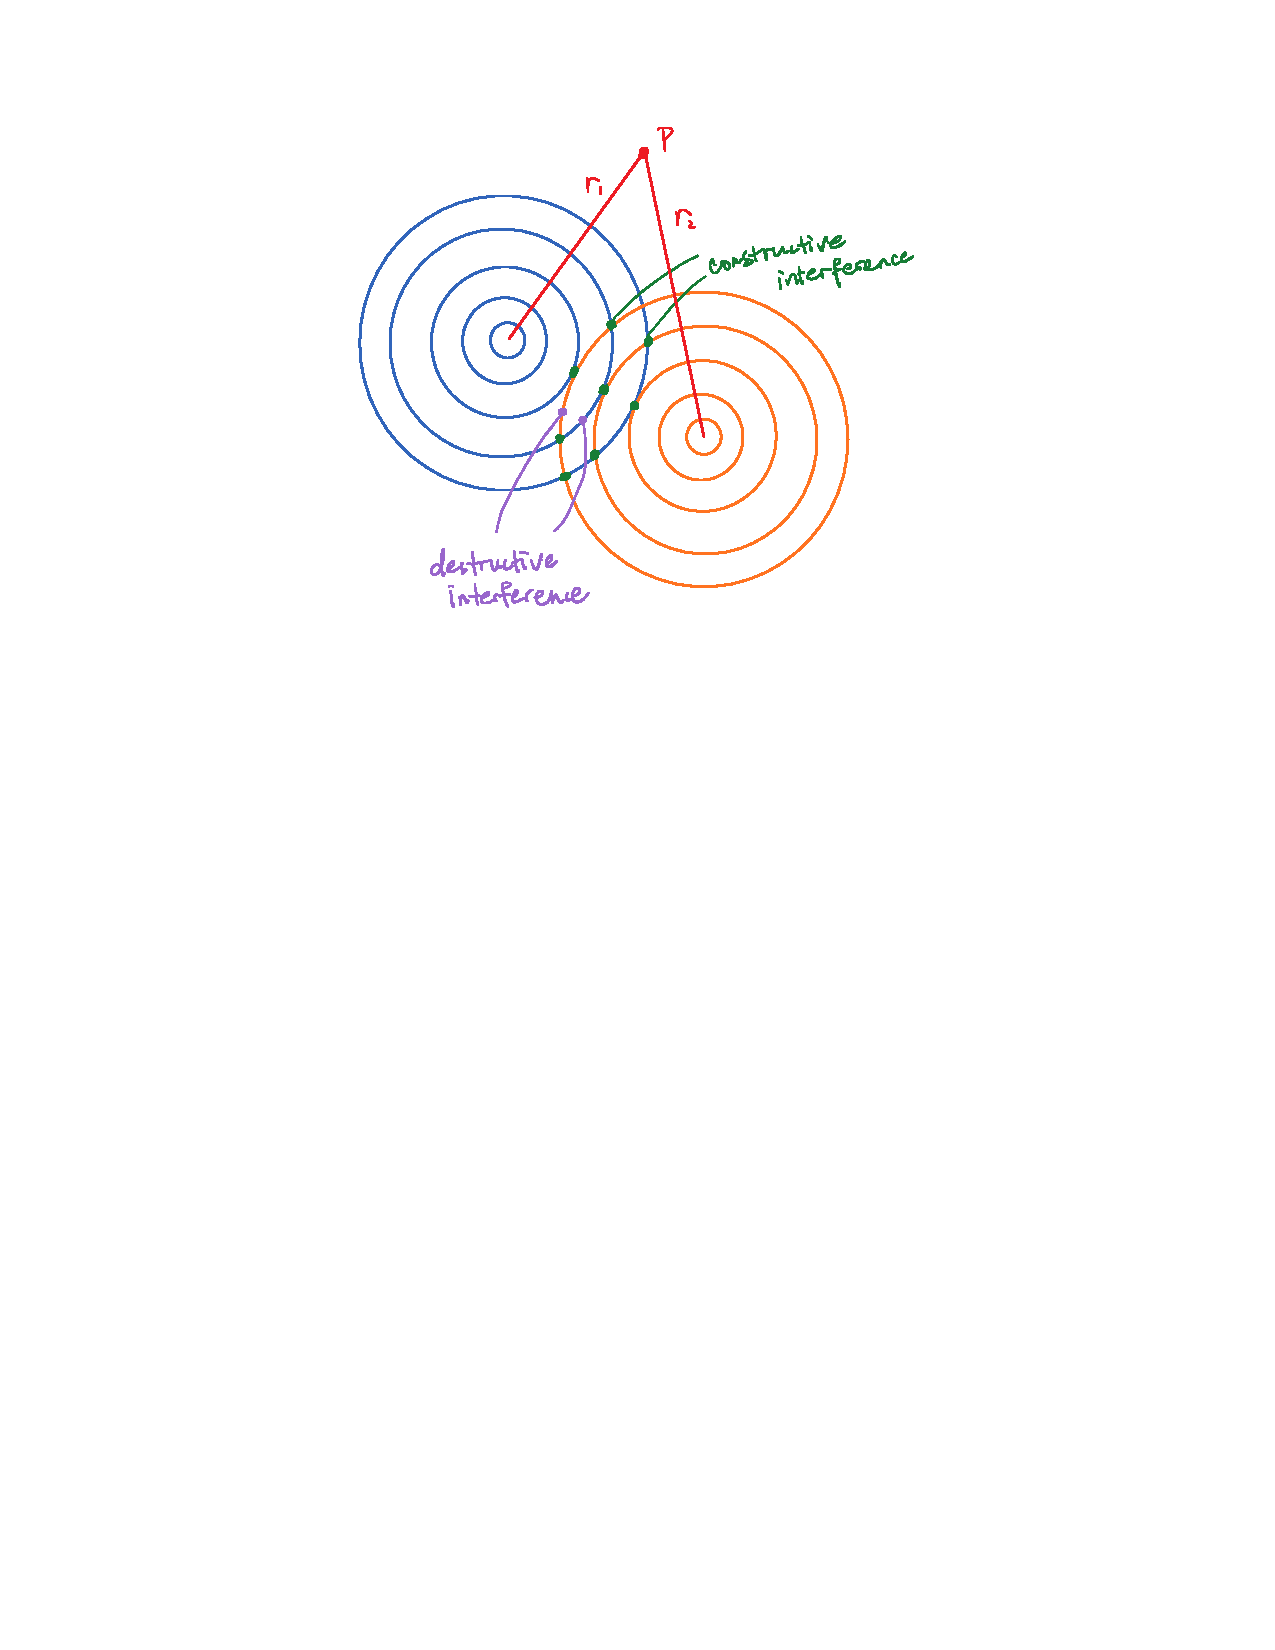
\includegraphics[scale=0.8]{inteference.pdf}
\end{center}
Constructive interference happens when the difference in travel distance is an integer times the wavelength, that is, for constructive interference, we have:
$$r_2 - r_1 = m\lambda \ \ \ \text{for some }m \in \Z$$
For destructive interference, the difference in travel distance is a half-integer times the wavelength, that is, for destructive interference, we have:
$$r_2 - r_1 = (m+\frac{1}{2}) \lambda \ \ \ \text{for some }m \in \Z$$
where $\lambda $ is the wavelength of the wave.\\

In general, the phase difference $\phi $ between waves from two coherent sources is given by:
$$\phi = k (r_2 - r_1) \ \ \ \text{with } k=\frac{2\pi}{\lambda}$$

Interference happens in electromagnetic waves too, the electromagnetic version of our wave example is called the Young's Experiment. \\

\newpage
\textbf{Young's Double Slit Experiment}\\
Set up: A light source on the left, a vertical double slit in the middle, and a screen on the right.\\

Here we shine light on a double slit. If light were only rays ant not waves, we should get only two bright spots on a screen behind the slit. Thomas Young claimed in 1799 that light was a wave, and demonstrated it definitely in his double slit experiment in 1801 through 1803. In fact, there are many bright spots observed on screen when the light is shine through the slits. The bright spots are the locations where constructive interference occur. The dark spots are the locations where the destructive interference occur. This suggests that light is wave-like. \\


We can characterize a point $P$ on the screen by the angle $\theta$. When $R >>d$, the vectors $\vec{r}_1$ and $\vec{r}_2$ are nearly parallel.  \\
\begin{center}
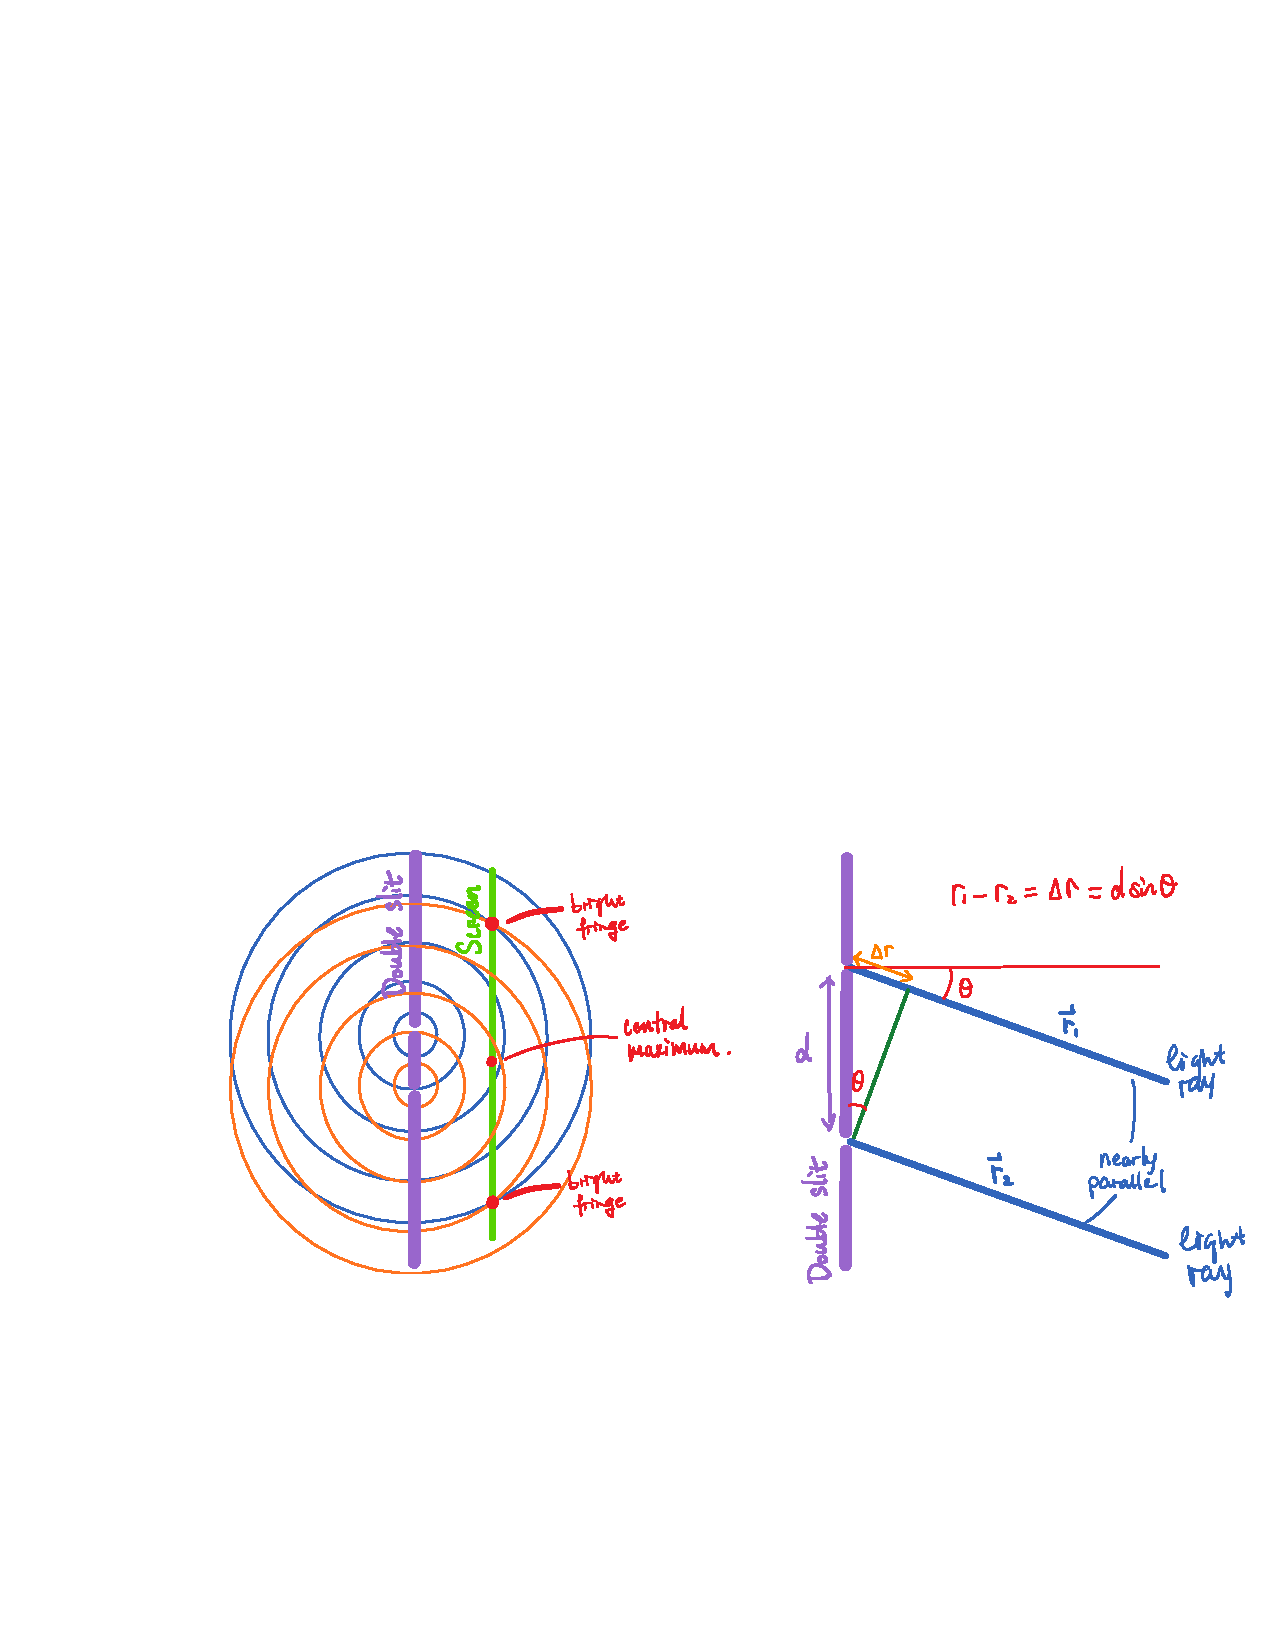
\includegraphics[scale=0.8]{doubleSlit.pdf}
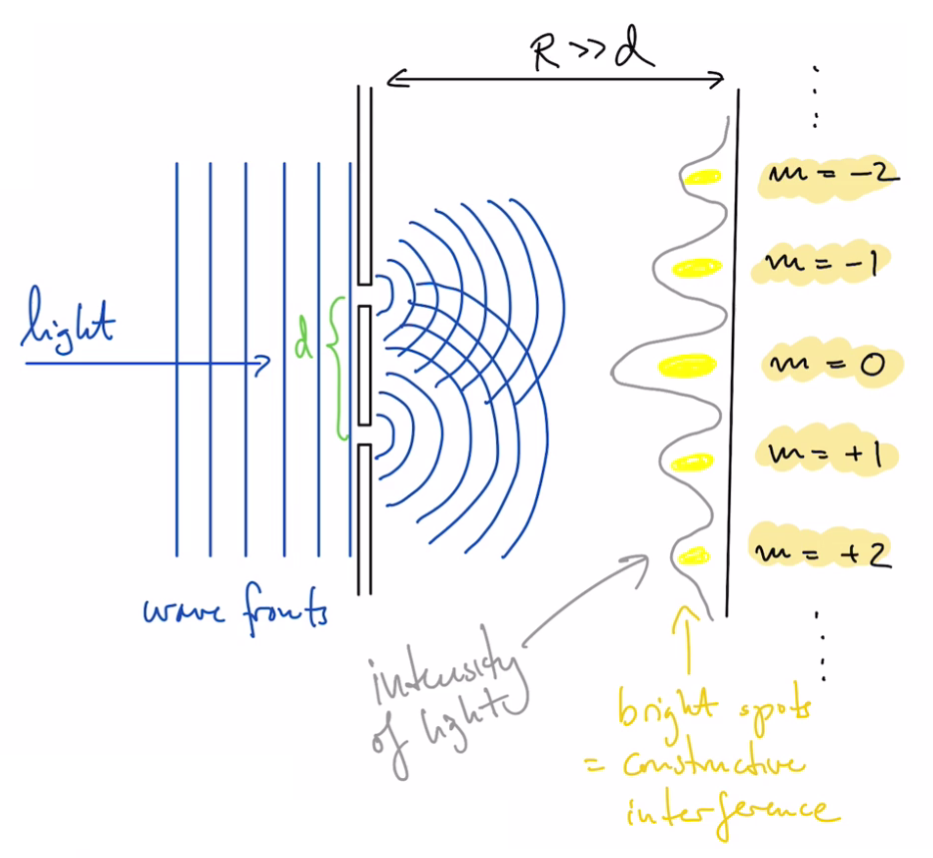
\includegraphics[scale=0.5]{douSlitInt.png}
\end{center}

On the screen in the Young Double Slit Experiment, we have high intensity on bright spots, and low intensity on dark fringes. The intensity of the wave is directly proportional to the power of the wave, which is directly proportional to the $($amplitude$)^2$ of the wave. For a sinusoidal electromagnetic wave, we have: $$E(x,t) = E_{max} \cos(kx-\omega t) \ \ \ \ \text{with } \frac{\omega}{k}=c$$
$$I = \frac{1}{2}\epsilon_0 c E_{max}^2$$
Suppose at some point $P$ on the screen, two sinusoidal waves are out-of-phase by $\phi$:
$$E_1(t) = E_0 \cos(\omega t+\phi)$$
$$E_2(t) = E_0 \cos(\omega t)$$
They interfere at $P$, with superposition principle, we can write the following:
$$E(t) = E_1(t) + E_2(t) = E_0(\cos(\omega t + \phi) + \cos(\omega t)) = 2E_0 \cos\left( \frac{\phi}{2}\right) \cos\left(\omega t + \frac{\phi}{2}\right)$$
Here we get the following:
$$E_{max} = 2E_0 \cos\left(\frac{\phi}{2} \right)$$
So the intensity of the wave can be described by the following:
$$I \propto E_{max}^2 = 4E_0^2 \cos^2\left( \frac{\phi}{2}\right)$$
Hence we get some conclusion here:
\begin{enumerate}
\item The maximum intensity of interference is 4 times greater than the individual wave maximum intensity
\item The minimum intensity is $0$ 
\item Average intensity is given by $2E_0^2$, and hence $I \propto 2E_0^2 =$ sum of the two intensities. \begin{center}
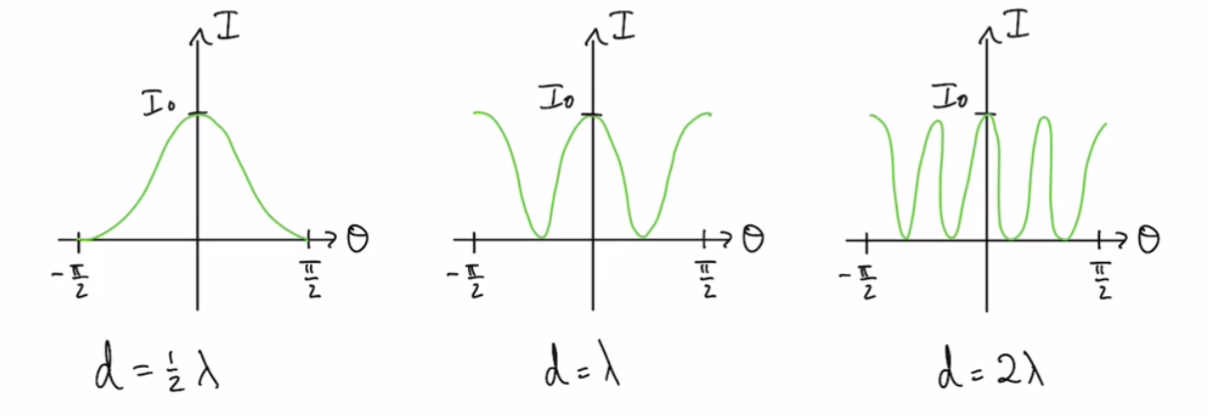
\includegraphics[scale=0.7]{waveInt.png}
\end{center}
\item Phase difference $\phi $ is the difference in path length of light. For coherent sources, $\phi = k(r_2-r_1) = k\, d\, \sin(\theta) = 2\pi \frac{d}{\lambda}\sin(\theta)$, so at point $P$, we can write the following:
$$I = 2\epsilon_0 cE_0^2 \cos^2\left( \pi \frac{d}{\lambda}\sin(\theta)\right)\qquad \text{with }-\frac{\pi}{2}<\theta<\frac{\pi}{2}$$
with $2\epsilon_0cE_0^2 = I_0$. This suggests that $I$ depends on the ratio of $\lambda$ and $d$. When $\lambda>>d$, we have $\frac{d}{\lambda}<<1$, hence we have: 
$$I = I_0\cos^2\left(\pi \frac{d}{\lambda}\sin(\theta)\right) \approx I_0 \left(1-\pi^2 \frac{d^2}{\lambda^2}\sin^2 (\theta)+\cdots \right) $$
so the interference pattern goes away when $\lambda >>d$. On the other hand, when we have $\lambda << d$, we have $\frac{d}{\lambda }>>1$, hence we have $I = I_0\cos^2\left(\pi \frac{d}{\lambda}\sin(\theta)\right)$, which gives very rapid oscillation as function of $\theta$. Again, in such case, the interference patter smears out and goes away. 
\end{enumerate}

Interference is observed in the double slit experiment when the distance $d$ between the slits is roughly of the same scale as the wavelength of light $\lambda$. Notice here, all peaks of the intensity derived above are the same, which does not match what we see from the data that the intensity of the fringe decreases as we move away from the central maximum. While the diffraction of light can explain the decrease in intensity of the light, with the following holds:
$$I = I_0 \left(\frac{\sin(\beta/2)}{\beta/2} \right)^2\qquad\qquad\qquad \beta = 2\pi \frac{a}{\lambda}\sin(\theta)$$
where $a$ is the size of a single slit. Here combining we get the following:
$$I = I_0 \left(\frac{\sin(\beta/2)}{\beta/2} \right)^2 \cos^2\left(\pi \frac{d}{\lambda}\sin(\theta)\right)$$

\newpage
\textbf{Polarization}\\

Suppose a wave is propagating in the $x$-direction. The choice of the orientation of $\vec{E}$ and $\vec{B}$ can be arbitrary provided that $\vec{E}\times \vec{B}$ has only the $\vec{x}$ component, and $\vec{E} \perp \vec{B}$. \\

Let:
$$\vec{E}_1 = \bmat{0\\E\\0}\qquad\qquad\qquad \vec{B}_1=\bmat{0\\0\\B}$$
$$\vec{E}_2 = \bmat{0\\0\\E}\qquad\qquad\qquad \vec{B}_2=\bmat{0\\-B\\0}$$
Light can also be circularly polarized, with the left and right polarized light defined by the following with respectively:
$$E_L = \vec{E}_1 + \vec{E}_2\qquad\qquad\qquad \vec{E}_R=\vec{E}_1-\vec{E}_2$$
Here $B_L$ and $B_R$ are defined accordingly to the orientation of $E_L$ and $E_R$. \\

The application of polarization of light includes sunglasses, wave filters in optics, stress tests of materials, reduce glare of car lights, and so on.\\


\newpage
Consider the Heat Equation:
\begin{align*}
\frac{\partial T}{\partial t} = \alpha \frac{\partial^2 T}{\partial x^2} \tag{1}
\end{align*}
where $\alpha $ is the thermal diffusivity of the material, which is proportional to thermal conductivity. Consider a system of a copper block, at time $t=0$, the left half of the block is at $100^\circ C$ and the right half of the block is at $0^\circ C$. Denote the left end of the block by $x=0$, the middle of the block as $x=1/2$. For cropper, the thermal diffusivity is $\alpha_{Cu} = 10^{-4}\, m^2/s$.\\

One class of solution to equation (1) is given by:
\begin{align*}
T_k(x,t) = \sin(kx)e^{-\alpha k^2 t}
\end{align*}

For the heat equation given by equation (1), the superposition principle applies, so in particular, we have: $$T(x,t)=b_0 + \sum_{m=1}^\infty b_m \sin(2\pi mx) e^{-\alpha(2\pi m)^2 t}$$
being a solution to equation (1), with $b_i\in \R$ being constants. Here we want to find $T(x,t)$ that satisfies our problem. Note that we can write the following:
\begin{align*}
T(x,0) = b_0 + \sin_{m=1}^\infty b_m \sin(2\pi mx) = \begin{cases}100^\circ C & 0<x<\frac{1}{2} \\ 0^\circ & 1/2 <x<1 \end{cases}
\end{align*}
One can verify that we have:
$$b_0 = \frac{T_0}{2}\qquad\qquad\qquad\qquad b_m = \begin{cases}\frac{2T_0}{\pi m} & m \text{ is odd}\\ 0 &m\text{ is even}\end{cases}$$
where $T_0 = 200^\circ$. Hence we have:
$$T(x,0) = 50^\circ C + \frac{200^\circ C}{\pi}\sum_{k=0}^\infty \frac{1}{2k+1}\sin(2\pi (2k+1) x)$$
We conclude the following:
$$T(x,t) = 50^\circ C + \frac{200^\circ C}{\pi}\sum_{k=0}^\infty \frac{1}{2k+1}\sin(2\pi (2k+1) x) e^{-\alpha (2\pi (2k+1))^2 t}$$



\end{document}

